%\chapter{Perturbation Theory}
\chapter{微扰理论}

我们在本章将注意力转向地球的自转、流体静力学椭率和横向不均匀性的影响。
在大多数全球地震学的应用中,特别对长周期,这些相对于球对称的偏离可以被视为{\em 微扰\/}。
\index{perturbation!slight}%
在这一状况下,可以用简正模式微扰理论来计算微扰后地球中的单态模式的本征频率和相应的本征函数,
以及对给定矩张量震源的简正模式微扰响应。
在本章中,我们將以一种普遍且非常理想化的观点来考虑球对称地球模型的任意微扰的效应。
简正模式微扰理论在长周期地震数据中的实际应用将在第14章有更详尽的讨论。
%%%

%\section{Isolated Mode}
\section{孤立模式}
\index{mode!isolated|(}%
\index{isolated mode|(}%

我们首要解决的基本问题是得到在地震频谱中较为孤立的模式的非简并本征频率的微扰。
这一经典的{\em 非简并\/}微扰问题的解是本章剩余部分要讨论的简并和准简并耦合模式理论的基础。
\index{perturbation!non-degenerate}%
\index{non-degenerate perturbation}%
我们首先忽略非弹性衰减的影响,来处理弹性非流体静力学地球模型的完全弹性微扰。
然后我们关注球对称流体静力学初始模型的特例,并进一步引入地球的微弱非弹性微扰。
如同第9章那样,最困难的是确定界面位置的微小变化的影响,
我们将遵循\textcite{woodhouse&dahlen78}所开创的处理方法。
%%%

%\subsection{Recapitulation}
\subsection{要点回顾}

我们仍然避免使用在第I部分中用来推导一般结果所使用的清楚但繁杂的符号。
一般无自转地球的本征频率和本征函数所满足的频率域动量方程及其相关边界条件~(\ref{4.nrmodeqn})--(\ref{4.bc4})用新的符号可以表示为
\eq
\label{13.nrmomeqn}
-\omega^{2\!}\rho\hspace{0.3 mm}\bs-\bdel\cdot\widetilde{\bT}
+\rho\bdel_{\!}\phi+\rho\hspace{0.3 mm}\bs\cdot\bdel\bdel\Phi=\bzero
\quad\mbox{在 $\earth$ 内},
\en
\eq
\bnh\cdot\widetilde{\bT}=\bzero\quad\mbox{在 $\p\earth$上},
\en
\eq
[\bnh\cdot\widetilde{\bT}]^+_-=\bzero\quad\mbox{在 $\Sigma_{\rm SS}$上},
\en
\eq
[\widetilde{\bt}]^+_-=\bnh[\bnh\cdot\widetilde{\bt}]^+_-
=\bzero\quad\mbox{在 $\Sigma_{\rm FS}$ 上}.
\en
第一類Piola-Kirchhoff应力增量$\widetilde{\bT}$和辅助矢量$\widetilde{\bt}$可以用位移本征函数$\bs$定义为
$\widetilde{\bT}=\bLambda\!:\!\bdel\bs$ 和
$\widetilde{\bt}=\bnh\cdot\widetilde{\bT}+\bdel^{\Sigma}\cdot(\varpi\bs)
-\varpi(\bdel^{\Sigma}\bs)\cdot\bnh$,
其中$\varpi=p-\bnh\cdot\btau\cdot\bnh$。
在无自转流体静力学地球中相应的方程和边界条件~(\ref{4.nrhydromom})--(\ref{4.hydrobc3})为
\eqa
\label{13.nrhydromom}
\lefteqn{
-\omega^{2\!}\rho\hspace{0.3 mm}\bs-\bdel\cdot\bT
+\bdel(\rho\hspace{0.3 mm}\bs\cdot\bdel\Phi)} \nonumber \\
&&\mbox{}\qquad\qquad
+\rho\bdel_{\!}\phi-[\bdel\cdot(\rho\hspace{0.3 mm}\bs)]\bdel\Phi=\bzero
\quad\mbox{在 $\earth$ 内},
\ena
\eq
\label{13.hydrobc1}
\bnh\cdot\bT=\bzero\quad\mbox{在 $\p\earth$ 上},
\en
\eq
\label{13.hydrobc2}
[\bnh\cdot\bT]^+_-=\bzero\quad\mbox{在 $\Sigma_{\rm SS}$ 上},
\en
\eq
\label{13.hydrobc3}
[\bnh\cdot\bT]^+_-
=\bnh[\bnh\cdot\bT\cdot\bnh]^+_-=\bzero
\quad\mbox{在 $\Sigma_{\rm FS}$ 上},
\en
其中$\bT=\bGamma\!:\!\bepsilon$。
不论在非流体静力学或流体静力学地球中,欧拉重力势函数增量$\phi$都是线性化泊松边界值问题的解
\eq
\label{13.fishy}
\bdel\cdot\bxi=0\quad\mbox{在 $\allspace$ 內},
\en
\eq
\label{13.fishybc}
[\phi]^+_-=0\quad\mbox{和}\quad[\bnh\cdot\bxi]^+_-=0
\quad\mbox{在 $\Sigma$ 上},
\en
其中 
$\bxi=(4\pi G)^{-1}\bdel_{\!}\phi+\rho\hspace{0.3 mm}\bs$.
此势函数问题的解为
\eq
\phi=-G\int_{\subearth}\frac{\rho'\bs'\cdot(\bx-\bx')}
{\|\bx-\bx'\|^3}\,dV',
\en
其中撇号表示在积分变量$\bx'$处取值。
地球自转的考虑可以通过在~(\ref{13.nrmomeqn})和~(\ref{13.nrhydromom})中加入科里奥利力项$2i\omega\bOmega\times\bs$并以重力势函数$\Phi+\psi$替代$\Phi$。

%\subsection{General elastic perturbation}
\subsection{一般弹性微扰}
\index{perturbation!elastic|(}%

扰动前的初始地球模型完全由其质量密度$\rho$和相应的重力势函数$\Phi$、初始流体静压强$p$和偏应力张量$\btau$、各向同性或各向异性的弹性张量$\bGamma$、及其内外界面的几何构形$\Sigma=\p\earth\cup\Sigma_{\rm SS}\cup\Sigma_{\rm FS}$所表述。
这些性质的微扰以如下形式给定:
\begin{enumerate}
\item[(1)]
\index{perturbation!density}%
密度受到扰动, $\rho\rightarrow\rho+\delta\hspace{-0.2 mm}\rho$;
\item[(2)]
\index{perturbation!gravitational}%
重力势函数也因此受到扰动,
$\Phi\rightarrow\Phi+\delta\Phi$;
\item[(3)] 
\index{perturbation!hydrostatic pressure}%
初始流体静力学压强受到扰动,
$p\rightarrow p+\delta p$;
\item[(4)]
\index{perturbation!deviatoric stress}%
偏应力也随即受到扰动,
$\btau\rightarrow\btau+\bdelta\btau$;
\item[(5)]
\index{perturbation!elastic}%
弹性张量受到扰动,
$\bGamma\rightarrow\bGamma+\bdelta\bGamma$;
\item[(6)]
\index{perturbation!boundary}%
最后,界面$\Sigma$在其本身法线方向上移动了$\delta\hspace{-0.1 mm}d$,
扰动的物理性质
$\rho+\delta\hspace{-0.2 mm}\rho$、$\Phi+\delta\Phi$、
$p+\delta p$、$\btau+\bdelta\btau$和
$\bGamma+\bdelta\bGamma$
通过在$\Sigma$附近的重新定义使其在扰动前的界面两侧是平滑的。
\end{enumerate}
由于地球模型的这些改变,非简并简正模式的本征频率$\omega$被扰动了$\delta\omega$,其对应的位移和势函数本征函数$\bs$和$\phi$分别被扰动了$\bdelta\bs$和 $\delta\phi$。
与物理性质一样,扰动后的场$\bs+\bdelta\bs$和
$\phi+\delta\phi$也通过在$\Sigma$附近的重新定义使其为在扰动前的界面两侧是平滑的。
我们将用$\Delta q$表示任何在扰动后边界上的扰动后量$q+\delta q$与相应的在扰动前边界上的扰动前量$q$之间的差异。
精确到微扰的一阶$\delta\hspace{-0.1 mm}d$,我们有
\eq
\label{13.deltaq1}
\Delta q=\delta q+\delta\hspace{-0.1 mm}d(\p_nq),
\en 
其中$\p_n=\bnh\cdot\bdel$表示法向导数,$q$可以是标量、矢量或任意阶张量。
由于位移而引起的边界法向$\bnh$的微扰为
\eq
\label{13.deltanhat}
\Delta\bnh=-\bdel^{\Sigma}(\delta\hspace{-0.1 mm}d).
\en
结合~(\ref{13.deltaq1})和~(\ref{13.deltanhat}),我们发现对于任何矢量或张量$\bq$有
\eq
\label{13.deltaq2}
\Delta q_n=\bnh\cdot\bdelta\bq+\delta\hspace{-0.1 mm}d(\p_nq_n)
-\bdel^{\Sigma}(\delta\hspace{-0.1 mm}d)\cdot\bq,
\en
其中 
$q_n=\bnh\cdot\bq$。
对于$\Sigma$上的任何标量、矢量或张量q,表面梯度$\bdel^{\Sigma}q=\bdel q-\bnh(\p_n q)$相应的微扰为
\eq
\label{13.deltaq3}
\Delta(\bdel^{\Sigma}q)=\bdel^{\Sigma}(\Delta
q)+[\bnh\bdel^{\Sigma}(\delta\hspace{-0.1 mm}d)
-\delta\hspace{-0.1 mm}d(\bdel^{\Sigma}\bnh)]\cdot\bdel^{\Sigma}q,
\en
地球模型的微扰$\delta\hspace{-0.2 mm}\rho$、$\delta\Phi$、$\delta p$、 $\bdelta\btau$和$\delta\hspace{-0.1 mm}d$不能被单独立地定义。
首先,重力势函数的微扰$\delta\Phi$必须是源于密度微扰$\delta\hspace{-0.2 mm}\rho$和界面位移$\delta\hspace{-0.1 mm}d$。$\delta\Phi$是边值问题的解
\eq
\label{13.pertbc1}
\del^2(\delta\Phi)=\left\{ \begin{array}{ll}
4\pi G_{\,}\delta\hspace{-0.2 mm}\rho &
\mbox{在 $\earth_{\rm S}$ 内} \\
0 & \mbox{在 $\allspace -\earth$ 内,}
\end{array}
\right.
\en
\eq
\label{13.pertbc4}
[\delta\Phi]^+_-=0\quad\mbox{和}\quad
[\bnh\cdot\bdel(\delta\Phi)+4\pi G\rho_{\,}
\delta\hspace{-0.1 mm}d]^+_-=0\quad
\mbox{在$\Sigma$上.}
\en
(\ref{13.pertbc1})--(\ref{13.pertbc4})的解可写成以下形式
\eq
\delta\Phi=-G\int_{\subearth}\frac{\delta\hspace{-0.2 mm}\rho'}{\|\bx-\bx'\|}\,
dV'
+G\int_{\Sigma}\frac{\delta\hspace{-0.1 mm}d'\,[\rho']^+_-}{\|\bx-\bx'\|}\,
d\/\Sigma',
\en
其中第一项来自密度微扰,而第二项来自界面位移。

此外,新的初始应力必须与新的重力体力达到力学平衡;
这就需要$\delta p$和$\bdelta\btau$满足微扰平衡条件
\eq
\label{13.delT0vol}
-\bdel(\delta p)+\bdel\cdot\bdelta\btau=\delta\hspace{-0.2 mm}\rho\bdel\Phi+
\rho\bdel_{\!}(\delta\Phi)\quad\mbox{在 $\earth$ 内},
\en
以及微扰连续性条件
$[\Delta(-\bnh p+\bnh\cdot\btau)]^+_-=\bzero$
或等价于
\eqa
\label{13.delT0bc}
\lefteqn{
[-\bnh_{\,}\delta p+\bnh\cdot\bdelta\btau]^+_-=
+\delta\hspace{-0.1 mm}d_{\,}[\bnh_{\,}\p_n p-\bnh\cdot\p_n\btau]^+_-} \nonumber \\
&&\mbox{}\qquad\qquad\qquad
+\bdel^{\Sigma}(\delta\hspace{-0.1 mm}d)
\cdot[-p\bI+\btau]^+_-\quad\mbox{在$\Sigma$上}.
\ena
在地球的液态区域$\earth_{\rm F}$,$\rho+\delta\hspace{-0.2 mm}\rho$、$\Phi+\delta\Phi$和$p+\delta p$的微扰后的等值面一定要重合,这强烈地限制了液体的密度和压强扰动$\delta\hspace{-0.2 mm}\rho$和$\delta p$的容许范围,
我们将会在第~\ref{13.sec.SNREI}节中对这一点加以讨论。

在地球的固态区域$\earth_{\rm S}$内,
我们可以任意给定弹性张量的微扰$\bdelta\bGamma$,只要满足弹性对称关系
$\delta\Gamma_{ijkl}
=\delta\Gamma_{jikl}=\delta\Gamma_{ijlk}=\delta\Gamma_{klij}$。
与之相应的联系第一类Piola-Kirchhoff应力增量$\widetilde{\bT}$与$\bdel\bs$的四阶张量微扰$\bdelta\bLambda$可以用$\bdelta\bGamma$、$\delta p$和 $\bdelta\btau$表示为
\eqa
\lefteqn{
\delta\Lambda_{ijkl}=\delta\Gamma_{ijkl}
-\delta p(\delta_{ij\,}\delta_{kl}-\delta_{il\,}\delta_{jk})
+\half(\delta\tau_{ij\,}\delta_{kl}
+\delta\tau_{kl\,}\delta_{ij}}
\nonumber \\
&&\mbox{}+\delta\tau_{ik\,}\delta_{jl}
-\delta\tau_{jk\,}\delta_{il}-\delta\tau_{il\,}\delta_{jk}
-\delta\tau_{jl\,}\delta_{ik}).
\ena
在液态区域$\earth_{\rm F}$,
微扰$\bdelta\bGamma$和$\bdelta\bLambda$的形式必须是
$\delta\Gamma_{ijkl}=\delta\hspace{-0.1 mm}\kappa_{\,}\delta_{ij\,}\delta_{kl}$
和 $\delta\Lambda_{ijkl}=\delta\hspace{-0.1 mm}\kappa_{\,}
\delta_{ij\,}\delta_{kl}
-\delta p(\delta_{ij\,}\delta_{kl}-\delta_{il\,}\delta_{jk})$,
其中$\delta\hspace{-0.1 mm}\kappa$为等熵不可压缩性的微扰。

我们还需要两个微扰
$\Delta\varpi$和$\Delta(\bdel^{\Sigma}\varpi)$,
其中 
$\varpi=p-\bnh\cdot\btau\cdot\bnh$;
前者为
\eqa
\label{13.Deltapinot}
\lefteqn{
\Delta\varpi=\delta p-\bnh\cdot\bdelta\btau\cdot\bnh
-\delta\hspace{-0.1 mm}d_{\,}(-\p_n p+\bnh\cdot\p_n\btau\cdot\bnh)} \nonumber \\
&&\mbox{}\qquad\qquad+2\bdel^{\Sigma}
(\delta\hspace{-0.1 mm}d)\cdot(\bnh\cdot\btau),
\ena
后者可以用~(\ref{13.deltaq3})得到:
\eq
\label{13.delgradpi}
\Delta(\bdel^{\Sigma}\varpi)=\bdel^{\Sigma}(\Delta
\varpi)+[\bnh\bdel^{\Sigma}(\delta\hspace{-0.1 mm}d)
-\delta\hspace{-0.1 mm}d(\bdel^{\Sigma}\bnh)]\cdot\bdel^{\Sigma}\varpi.
\en
由于初始牵引力$-p\bnh+\bnh\cdot\btau$的连续性和边界条件~(\ref{13.delT0bc},
$\Delta\varpi$在界面$\Sigma$上是连续的:$[\Delta\varpi]^+_-=0$。

%\subsection{Application of Rayleigh's principle}
\subsection{瑞利原理的应用}
\index{Rayleigh's principle!application of|(}%
\label{13.sec.Rayprin}
利用瑞利变分原理可以确定非简并本征频率的一阶微扰$\delta\omega$,
而无需同时求解相应的本征函数微扰。
如果将$\bdelta\bs$和$\delta\phi$视为相互独立的微扰,计算会不那么复杂;
我们采用此种观点,并在下面的推导中使用位移-势函数形式的瑞利原理。
与球对称微扰的情形一样,基本的策略是将修改后的作用量$\sI'$
\index{action!modified}%
\index{modified action}%
视为不仅仅是本征函数$\bs$和$\phi$的泛函,同时也是相应的本征频率$\omega$和描述地球模型所需要的所有参数的泛函。
我们用$\earth$来代表体积上的地球模型参数$\rho$、$\bLambda$和 $\bdel\bdel\Phi$的集合,
同时用$\earth^{\Sigma}$代表面积上的地球模型参数$\varpi$、 $\bdel^{\Sigma}\varpi$和$\bnh$的集合。
这样一来,$\sI'$的全部依赖性可以通过将~(\ref{4.IPRDEF})写为如下形式来明确表达
\eq
\label{13.pertact}
\sI'=\int_{\subspace}L'(\bs,\bdel\bs,\bdel_{\!}\phi;
\omega,\earth)\,dV
+\int_{\Sigma}[L^{\Sigma}(\bs,\bdel^{\Sigma}\bs;
\earth^{\Sigma})]^+_-\,d\Sigma,
\en
其中
\eqa
\label{13.Ldef}
\lefteqn{
L'=\half[\omega^{2\!}\rho\hspace{0.3 mm}\bs\cdot\bs
-\bdel\bs\!:\!\bLambda\!:\!\bdel\bs
-2\rho\hspace{0.3 mm}\bs\cdot\bdel_{\!}\phi} \nonumber \\
&&\mbox{}\qquad\qquad-\rho\hspace{0.3 mm}
\bs\cdot\bdel\bdel\Phi\cdot\bs
-(4\pi G)^{-1}\bdel_{\!}\phi\cdot\bdel_{\!}\phi],
\ena
\eq
\label{13.Lsigdef}
L^{\Sigma}=\half[(\bnh\cdot\bs)\bdel^{\Sigma}\cdot(\varpi\bs)
-\varpi\hspace{0.3 mm}\bs\cdot(\bdel^{\Sigma}\bs)\cdot\bnh].
\en
为简洁起见,我们将把接下来推导中出现的所有界面上的面积分\textcolor{red}{写为
$\Sigma=\p\earth\cup\Sigma_{\rm SS}\cup\Sigma_{\rm FS}$};
然而,要注意~(\ref{13.pertact})中的积分实际上仅在固-液不连续面$\Sigma_{\rm FS}$上,
因为表面拉格朗日量密度在$\p\earth$和$\Sigma_{\rm SS}$上均为连续的,即$[L^{\Sigma}]^+_-=0$。
\index{Lagrangian density!volumetric}%
\index{Lagrangian density!surface}%
 
对于扰动前地球模型的每一组本征解$\omega$、$\bs$、$\phi$,其修改后的作用量为
\eq
\label{13.action0}
\sI'=0.
\en
与第9章一样,我们考虑~(\ref{13.action0})式相对于所有变量$\omega$、
$\earth$和$\earth^{\Sigma}$的{\em 全变分\/},
\index{total variation}%
包括$\omega$、
$\earth$和$\earth^{\Sigma}$:
\eqa
\label{13.delItot}
\lefteqn{
\delta\sI_{\rm total}^{\prime}=
\int_{\subearth}[\bdelta\bs\cdot(\partial_{\subs}
L')+\bdel(\bdelta\bs)\cdot(\partial_{\sbdel\subs}L')]\/dV} \nonumber \\
&&\mbox{}+\int_{\subspace}\bdel(\delta\phi
)\cdot(\partial_{\sbdel_{\!}\phi}L')\,dV \nonumber \\
&&\mbox{}+\int_{\subearth}[\delta\omega(\partial_{\omega}L')+\delta\earth
(\p_{\subearth}L')]\,dV \nonumber \\
&&\mbox{}+\int_{\Sigma}[\Delta\bs\cdot(\p_{\subs}L^{\Sigma})+
\Delta(\bdel^{\Sigma}\bs)\!:\!(\p_{\sbdel^{\Sigma}\subs}
L^{\Sigma})]^+_-\,d\/\Sigma \nonumber \\
&&\mbox{}+\int_{\Sigma}[\Delta\earth^{\Sigma}
(\p_{\subearth^{\Sigma}}L^{\Sigma})
+\delta\hspace{-0.1 mm}d(\bdel\cdot\bnh)L^{\Sigma}
-\delta\hspace{-0.1 mm}d_{\,}L']^+_-\,d\/\Sigma=0.
\ena
这里我们引入了表示相对于地球模型参数的变分的缩写符号$\delta\earth(\p_{\subearth}L')$和$\Delta\earth^{\Sigma}(\p_{\subearth^{\Sigma}}L^{\Sigma})$:
\eqa
\label{13.volkern}
\lefteqn{
\delta\earth
(\p_{\subearth}L')=
\delta\hspace{-0.2 mm}\rho(\p_{\!\subrho}L')
+\bdelta\bLambda\tdot
(\p_{\hspace{-0.1mm}\subLambda} L')}\nonumber \\
&&\mbox{}\qquad\qquad\qquad
+\bdel\bdel(\delta\Phi)\!:\!(\p_{\sbdel\sbdel_{\!}\Phi}L'),
\ena
\eqa
\lefteqn{
\Delta\earth^{\Sigma}(\p_{\subearth
^{\Sigma}}L^{\Sigma})=\Delta\varpi(\p_{\varpi}L^{\Sigma})
+\Delta(\bdel^{\Sigma}\varpi)\cdot(\p_{\sbdel^{\Sigma}\varpi}
L^{\Sigma})} \nonumber \\
&&\mbox{}\qquad\qquad\qquad
+\Delta\bnh\cdot(\p_{\subnhat}L^{\Sigma}).
\ena
(\ref{13.delItot})中第一和第三个体积分的积分区域是地球的体积$\earth$,而非全空间$\allspace$,
这是因为只有包含$\bdel_{\!}\phi\cdot\bdel_{\!}\phi$的项在地球外部$\allspace -\earth$是非零的。
最后一个面积分的最后一项$-\delta\hspace{-0.1 mm}d_{\,}L'$源于因界面移动而引起的体积分积分区域的微扰,
而倒数第二项则源于相应的微分面积元微扰:
$\Delta(d\/\Sigma)=\delta\hspace{-0.1 mm}d(\bdel\cdot\bnh)\,d\/\Sigma$。
将二维和三维形式的高斯定理应用于~(\ref{13.delItot}),我们得到
\eqa
\label{13.manyints}
\lefteqn{\delta\sI_{\rm total}^{\prime}=
\int_{\subearth}\bdelta\bs\cdot[\p_{\subs}
L'-\bdel\cdot(\p_{\sbdel\subs}L')]\,dV} \nonumber \\
&&\mbox{}+\int_{\Sigma}[\bdelta\bs\cdot\{\p_{\subs}L^{\Sigma}
-\bdel^{\Sigma}\cdot(\p_{\sbdel^{\Sigma}\subs}L^{\Sigma})
-\bnh\cdot(\p_{\sbdel\subs}L')\}]^+_-\,d\/\Sigma \nonumber \\
&&\mbox{}-\int_{\subspace}\delta\phi_{\,}
[\bdel\cdot(\p_{\sbdel_{\!}\phi}L')]\,dV
-\int_{\Sigma}[\delta\phi\,\{
\bnh\cdot(\p_{\sbdel_{\!}\phi}L')\}]^+_-\,d\/\Sigma \nonumber \\
&&\mbox{}+\int_{\Sigma}\delta\hspace{-0.1 mm}d_{\,}
[\p_n\bs\cdot\{\p_{\subs}L^{\Sigma}
-\bdel^{\Sigma}\cdot(\p_{\sbdel^{\Sigma}\subs}L^{\Sigma})
\}]^+_-\,d\/\Sigma \nonumber \\
&&\mbox{}+\int_{\Sigma}[\{\bnh\bdel^{\Sigma}(\delta\hspace{-0.1 mm}d)
-\delta\hspace{-0.1 mm}d(\bdel^{\Sigma}\bnh)\}\cdot
(\bdel^{\Sigma}\bs)\!:\! (\p_{\sbdel^{\Sigma}\subs}L^{\Sigma})]^+_-\,d\/\Sigma
\nonumber \\
&&\mbox{}+\int_{\subearth}[\delta\omega(\partial_{\omega}L')+\delta\earth
(\p_{\subearth}L')]\,dV \nonumber \\
&&\mbox{}+\int_{\Sigma}[\Delta\earth^{\Sigma}
(\p_{\subearth^{\Sigma}}L^{\Sigma})
+\delta\hspace{-0.1 mm}d_{\,}(\bdel\cdot\bnh)L^{\Sigma}
-\delta\hspace{-0.1 mm}d_{\,}L']^+_-\,d\/\Sigma=0.
\ena
包含本征频率微扰$\delta\omega$的项简单就是
\eq
\label{13.NORMAL}
\delta\omega\int_{\subearth}\p_{\omega}L'\,dV=\omega_{\,}\delta\omega
\int_{\subearth}\rho\,\bs\cdot\bs\,dV=\omega_{\,}\delta\omega,
\en
这里我们引入了归一化条件~(\ref{4.ANORMAL})来得到最后一个等式。
我们将所寻求的量留在~(\ref{13.NORMAL})的左边,将所有其它项移至右边,并加以合并。
(\ref{13.manyints})式中所有包含微扰
$\bdelta\bs$和$\delta\phi$的体积分均为零,
与在第~\ref{4.sec.Rayprin}节中位移-势函数形式瑞利原理的推导完全一样,
因为$\p_{\subs}L'-\bdel\cdot(\p_{\sbdel\subs}L')=\bzero$
和$\bdel\cdot(\p_{\sbdel_{\!}\phi}L')=0$这两个量
分别是频率域的动量方程~(\ref{13.nrmomeqn})和泊松方程~(\ref{13.fishy})。
然而,前两个面积分在这里并不为零,因为界面的位移$\delta\hspace{-0.1 mm}d$使得$\bdelta\bs$和$\delta\phi$成为{\em 不可容许}的变化。
\index{admissible variation}%

在第一个面积分中与$\bdelta\bs$相乘的量
$\p_{\subs}L^{\Sigma}
-\bdel^{\Sigma}\cdot(\p_{\sbdel^{\Sigma}\subs}L^{\Sigma})
-\bnh\cdot(\p_{\sbdel\subs}L')$
仍然等于$\widetilde{\bt}$,但由于界面微扰$\delta\hspace{-0.1 mm}d$,
$[\bdelta\bs\cdot\widetilde{\bt}]^+_-=0$不再成立。
在固-固界面$\Sigma_{\rm SS}$上,我们必须有$[\Delta\bs]^+_-=\bzero$,或等价地
\eq
\label{13.hyneed1}
[\bdelta\bs]^+_-=-\delta\hspace{-0.1 mm}d_{\,}[\p_n\bs]^+_-,
\en
而在固-液界面$\Sigma_{\rm FS}$上,我们必须有
$[\Delta(\bnh\cdot\bs)]^+_-=0$,或等价地
\eq
\label{13.hyneed2}
[\bnh\cdot\bdelta\bs]^+_-=-\delta\hspace{-0.1 mm}d_{\,}[\p_ns_n]^+_-
+\bdel^{\Sigma}(\delta\hspace{-0.1 mm}d)\cdot[\bs]^+_-.
\en
因为$\widetilde{\bt}$在所有$\Sigma$上连续,且为$\Sigma_{\rm FS}$的法向矢量,
故在所有界面上我们有:
\eq
\label{13.pertBC1}
[\bdelta\bs\cdot\widetilde{\bt}]^+_-=-\delta\hspace{-0.1 mm}d_{\,}
[\widetilde{\bt}\cdot\p_n\bs]^+_-
+\bdel^{\Sigma}(\delta\hspace{-0.1 mm}d)\cdot[(\bnh\cdot\widetilde{\bt})\bs]^+_-.
\en
我们仍然有$\p_{\sbdel_{\!}\phi}L=-\bxi$,但$[\delta\phi(\bnh\cdot\bxi)]^+_-=0$不再成立。
微扰后的势函数边界条件为
$[\Delta\phi]^+_-=0$,
或等价于
\eq
\label{13.hyneed3}
[\delta\phi]^+_-=-\delta\hspace{-0.1 mm}d_{\,}[\p_n\phi]^+_-.
\en
此式再加上$\bnh\cdot\bxi$的连续性使我们有
\eq
\label{13.pertBC3}
[\delta\phi(\bnh\cdot\bxi)]^+_-=
-\delta\hspace{-0.1 mm}d_{\,}[(\bnh\cdot\bxi)\p_n\phi]^+_-.
\en
(\ref{13.pertBC1})和~(\ref{13.pertBC3})这两个条件正是计算(\ref{13.manyints})中前两个面积分所需要的关系式。
其余六个积分仅依赖于体积上和面积上的地球模型参数微扰$\delta\earth$和$\Delta\earth^{\Sigma}$,
而不依赖于本征函数微扰$\bdelta\bs$和$\delta\phi$,因此可以直接使用~(\ref{13.Ldef})和~(\ref{13.Lsigdef})中的$L'$和$L^{\Sigma}$来计算。
%%%

通过一些努力,本征频率微扰$\delta\omega$的最终一阶结果可以表示成如下形式
\eqa
\label{13.delomeqn}
\lefteqn{\delta\omega=\frac{1}{2\om}\int_{\subearth}
[\delta\hspace{-0.2 mm}\rho_{\,}(-\omega^2\bs\cdot\bs+2\bs\cdot\bdel_{\!}\phi
+\bs\cdot\bdel\bdel\Phi\cdot\bs)} \nonumber \\
&&\qquad\qquad+\bdel\bs\!:\!\bdelta\bLambda\!:\!\bdel\bs
+\rho\hspace{0.3 mm}\bs\cdot\bdel\bdel(\delta\Phi)\cdot\bs]\,dV \nonumber \\
&&\mbox{}\!\!\!+\frac{1}{2\om}\int_{\Sigma}\delta\hspace{-0.1 mm}d_{\,}
[2L'+2(\bnh\cdot\widetilde{\bT})\cdot\p_n\bs+2(\bnh\cdot\bxi)
\p_n\phi \nonumber \\
&&\mbox\qquad\qquad
+\varpi\hspace{0.3 mm}\{(\bdel^{\Sigma}\bs)\!:\!(\bdel^{\Sigma}\bs)^{\rm T}
-(\bdel^{\Sigma}\cdot\bs)^2\} \nonumber \\
&&\mbox{}\qquad\qquad\qquad+(\bdel^{\Sigma}\varpi)
\cdot\{s_n(\bs\cdot\bdel^{\Sigma}\bnh)
-\bs(\bdel^{\Sigma}\cdot\bs)\} \nonumber \\
&&\mbox{}\qquad\qquad\qquad\qquad-(\bdel^{\Sigma}
\bdel^{\Sigma}\varpi)\!:_{\!}\bs\bs]^+_-\,d\/\Sigma \nonumber \\
&&\mbox{}\!\!\!-\frac{1}{2\om}\int_{\Sigma_{\rm FS}}
\bdel^{\Sigma}(\delta\hspace{-0.1 mm}d)\cdot
[2(\bnh\cdot\widetilde{\bt})\bs]^+_-\,d\/\Sigma \nonumber \\
&&\mbox{}\!\!\!+\frac{1}{2\om}\int_{\Sigma_{\rm FS}}
\Delta\varpi_{\,}[2(\bs\cdot\bdel^{\Sigma}s_n)-
\bs\cdot(\bdel^{\Sigma}\bnh)\cdot\bs]^+_-\,d\/\Sigma.
\ena
(\ref{13.delomeqn})式使得我们可以利用扰动前的本征函数$\bs$和$\phi$以及地球模型的各种微扰来明确计算$\delta\omega$。
第一个积分源于体积上的密度微扰$\delta\hspace{-0.2 mm}\rho$、联系第一类Piola-Kirchhoff应力增量$\widetilde{\bT}$与$\bdel\bs$的四阶张量微扰$\bdelta\bLambda$,以及重力势函数微扰$\delta\Phi$的影响;而接下来的两个积分则来自界面位置微扰$\delta\hspace{-0.1 mm}d$的影响。如~(\ref{13.Deltapinot})所示,
最后一个积分中的微扰$\Delta\varpi$还依赖于$\delta\hspace{-0.1 mm}d$、
$\delta p$和$\bdelta\btau$。
在$\Sigma$上的积分中包含法向牵引力$\varpi$的所有项,在$\p\earth$和$\Sigma_{\rm SS}$上都是连续的;
因此,与包含$\bdel^{\Sigma}(\delta\hspace{-0.1 mm}d)$和$\Delta\varpi$的积分一样,它们的计算只需要在固-液边界$\Sigma_{\rm FS}$上进行。
在对面积分的化简中,我们利用了~(\ref{13.deltanhat})
和~(\ref{13.delgradpi})、曲率张量的对称性
$\bdel^{\Sigma}\bnh=(\bdel^{\Sigma}\bnh)^{\rm T}$、
以及很容易证明的表面梯度等式
$\bdel^{\Sigma}\bdel^{\Sigma}-\bnh(\bdel^{\Sigma}\bnh)\cdot\bdel^{\Sigma}=
[\bdel^{\Sigma}\bdel^{\Sigma}-\bnh(\bdel^{\Sigma}\bnh)\cdot
\bdel^{\Sigma}]^{\rm T}$。
\index{Rayleigh's principle!application of|)}%


%\subsection{Hydrostatic starting model}
\subsection{流体静力学初始模型}
\index{hydrostatic Earth|(}%
\index{starting model!hydrostatic|(}%
\index{Earth model!hydrostatic|(}%

如果初始模型是扰动前初始应力为$-p\hspace{0.2 mm}\bI$的流体静力学模型,则上述结果可以大大地简化。
此时初始应力微扰为$-\delta p_{\,}\bI+\btau$,其中$\btau$是总的偏应力。
由于地球中任何地方的偏应力都非常小,因此视其为微扰是一个很好的近似。
边界条件~(\ref{13.delT0bc})退化为$[-\bnh_{\,}\delta p+\bnh\cdot\btau]^+_-=
\delta\hspace{-0.1 mm}d_{\,}\bnh[\p_np]^+_-$。
$\varpi$只是初始压强$p$,而其微扰~(\ref{13.Deltapinot})则成为
$\Delta\varpi=\delta p-\bnh\cdot\btau\cdot\bnh+\delta\hspace{-0.1 mm}d(\p_np)$。
因为$\varpi$在$\Sigma_{\rm FS}$上为常数,
(\ref{13.delomeqn})中包含表面梯度的项
$\bdel^{\Sigma}\varpi$和
$\bdel^{\Sigma}\bdel^{\Sigma}\varpi$
均为零。
此外,固-液边界不能承受任何剪切牵引力,因此在$\Sigma_{\rm FS}$上
必须有$\bnh\cdot\btau=\bnh(\bnh\cdot\btau\cdot\bnh)$。
经过冗长的推导可以化简(\ref{13.delomeqn})中的其它项,并得到本征频率微扰的最简便的表达式;
这一努力的结果最终可以用类似于~(\ref{eq:9.delomiso})--(\ref{eq:9.Kd})的Fr\'{e}chet积分核符号来表示:
\eqa
\label{13.hydrtonon}
\lefteqn{\delta\omega=
\int_{\subearth}\delta\earth\hspace{0.3 mm}K_{\subearth}
\,dV+\int_{\Sigma}\delta\hspace{-0.1 mm}d_{\,}[K_{\rm d}]^+_-\,d\/\Sigma} \\
&&\mbox{}+\int_{\Sigma_{\rm FS}}\bdel^{\Sigma}
(\delta\hspace{-0.1 mm}d)\cdot[\bK_{\rm d}
]^+_-\,d\/\Sigma+\int_{\subearth_{\rm S}}\btau\!:\!\bK_{\subtau}
\,dV
\nonumber \\
&&\mbox{}\qquad+\int_{\Sigma_{\rm FS}}
(\bnh\cdot\btau)\cdot[\bK_{\subtau}^{\Sigma}
]^+_-\,d\/\Sigma+\int_{\Sigma_{\rm FS}}\bdel^{\Sigma}(\Delta\varpi)\cdot
[\bK_{\varpi}]^+_-\,d\/\Sigma, \nonumber
\ena
其中
\eqa
\label{13.hydrvlper}
\lefteqn{2\omega\hspace{0.3 mm}\delta\earth\hspace{0.3 mm}K_{\subearth}=
\delta\hspace{-0.2 mm}\rho\hspace{0.3 mm}[-\omega^2\bs\cdot\bs
+2\bs\cdot\bdel_{\!}\phi+\bs\cdot\bdel\bdel\Phi\cdot\bs} \nonumber \\
&&\mbox{}
+\bdel\Phi\cdot(\bs\cdot\bdel\bs
-\bs\bdel\cdot\bs)]+\beps\!:\!\bdelta\bGamma\!:\!\beps \nonumber \\
&&\mbox{}\qquad+\rho\bdel(\delta\Phi)
\cdot(\bs\cdot\bdel\bs
-\bs\bdel\cdot\bs)
+\rho\hspace{0.3 mm}\bs\cdot\bdel\bdel(\delta\Phi)\cdot\bs,
\ena
\vspace{-5.0 mm}
\eqa
\label{13.Hsighydr}
\lefteqn{2\omega K_{\rm d}=\rho\hspace{0.2 mm}[
\omega^2\bs\cdot\bs
-2\bs\cdot\bdel_{\!}\phi
-\bs\cdot\bdel\bdel\Phi\cdot\bs} \nonumber \\
&&\mbox{}-\bdel\Phi\cdot(\bs\cdot\bdel\bs
-\bs\bdel\cdot\bs)]
-\beps\!:\!\bGamma\!:\!\beps
-(4\pi G)^{-1}\bdel_{\!}\phi\cdot\bdel_{\!}\phi \nonumber \\
&&\mbox{}\qquad
+2(\bnh\cdot\bT)\cdot\p_n\bs
+2(\bnh\cdot\bxi)\p_n\phi,
\ena
\eq
\label{13.boldHdef}
2\omega\bK_{\rm d}=-
2(\bnh\cdot\bT\cdot\bnh)\bs,
\en
\vspace{-2.5 mm}
\eqa \label{13.Ksubtau}
\lefteqn{2\omega\bK_{\subtau}=
\bs\cdot\bdel\bdel\bs
-\bs\bdel(\bdel\cdot\bs)} \nonumber \\
&&\mbox{}+\half\bdel\bs\cdot(\bdel\bs)^{\rm T}
-\half(\bdel\bs)^{\rm T}\cdot\bdel\bs,
\ena
\eq
\label{13.taukern2}
2\omega\bK_{\subtau}^{\Sigma}
=s_n(\p_n\bs)-\bs(\p_ns_n),
\en
\eq
\label{13.taukern3}
2\omega\bK_{\varpi}=-s_n\bs.
\en
(\ref{13.hydrtonon})中第一项表示密度微扰$\delta\hspace{-0.2 mm}\rho$、
弹性张量微扰$\bdelta\bGamma$和引力势函数微扰$\delta\Phi$的一阶效应,
第二和第三项源于界面$\Sigma$的位移$\delta\hspace{-0.1 mm}d$,
而第四和第五项则来自在$\earth_{\rm S}$内和$\Sigma_{\rm FS}$上的初始偏应力$\btau$。
最后的第六项也与偏应力有关;然而,它完全可以用在$\earth_{\rm F}$内的压强微扰$\delta p$来计算,因为$\Delta\varpi$在$\Sigma_{\rm FS}$上是连续的。
\index{starting model!hydrostatic|)}%

\renewcommand{\thesubsection}{$\!\!\!\raise1.3ex\hbox{$\star$}\!\!$
\arabic{chapter}.\arabic{section}.\arabic{subsection}}
%\subsection{Hydrostatic perturbation}
\subsection{流体静力学微扰}
\index{perturbation!hydrostatic|(}%
\index{hydrostatic perturbation|(}%
\renewcommand{\thesubsection}{\arabic{chapter}.\arabic{section}.\arabic{subsection}}

如果最终和初始模型均为流体静力学模型,因而$\btau=\bzero$,则本征频率微扰$\delta\omega$简化为
\eqa
\label{13.hydrohydro}
\lefteqn{\delta\omega=
\int_{\subearth}\delta\earth\hspace{0.3 mm}K_{\subearth}
\,dV+\int_{\Sigma}\delta\hspace{-0.1 mm}d_{\,}
[K_{\rm d}]^+_-\,d\/\Sigma} \nonumber \\
&&\mbox{}\qquad\qquad
+\int_{\Sigma_{\rm FS}}\bdel^{\Sigma}
(\delta\hspace{-0.1 mm}d)\cdot[\bK_{\rm d}
]^+_-\,d\/\Sigma.
\ena
在(\ref{13.hydrtonon})中,除了包含$\btau$的项为零以外,由于在$\Sigma_{\rm FS}$上$\bdel^{\Sigma}(\Delta\varpi)=\bzero$,因此最后一个面积分也为零。
\index{quasi-hydrostatic approximation}%
值得注意的是,没有必要给定初始模型中的初始静压强$p$或压强微扰$\delta p$;
需要考虑的微扰仅有$\delta\hspace{-0.2 mm}\rho$、$\bdelta\bGamma$、
$\delta\Phi$和$\delta\hspace{-0.1 mm}d$。
严格来说,(\ref{13.hydrohydro})仅适用于初始和最终模型都是无自转的流体静力学球体;但更一般而言,它也可以用来确定准流体静力学近似下一般非流体静力学微扰的影响。

将瑞利原理应用于{\em 流体静力学\/}地球模型的修改后作用量$\sI'$,我们也可以得到~(\ref{13.hydrohydro})。我们将~(\ref{4.hydroact2})改写成如下形式
\eq
\label{13.hyperact}
\sI'=\int_{\subspace}L'(\bs,\bdel\bs,
\bdel_{\!}\phi;\omega,\earth)\,dV=0,
\en
其中符号$\earth$在此表示流体静力学地球模型参数
$\rho$、$\bGamma$、$\bdel\Phi$和$\bdel\bdel\Phi$的集合,
而修改后的拉格朗日量密度$L'$为
\eqa
\label{13.ZOOT}
\lefteqn{L'=\half[\omega^{2\!}\rho\hspace{0.3 mm}\bs\cdot\bs
-\beps\!:\!\bGamma\!:\!\beps
-2\rho\hspace{0.3 mm}\bs\cdot\bdel_{\!}\phi-\rho
\hspace{0.3 mm}\bs\cdot\bdel\bdel\Phi\cdot\bs} \nonumber \\
&&\mbox{}-\rho\bdel\Phi\cdot(\bs\cdot\bdel\bs
-\bs\bdel\cdot\bs)
-(4\pi G)^{-1}
\bdel_{\!}\phi\cdot\bdel_{\!}\phi].
\ena
相对于其所有变量的全变分~(\ref{13.hyperact})为
\index{total variation}%
\eqa
\label{13.hydelItot}
\lefteqn{
\delta\sI^{\prime}_{\rm total}=
\int_{\subearth}[\bdelta\bs\cdot(\partial_{\subs}
L')+\bdel(\bdelta\bs)
\cdot(\partial_{\sbdel\subs}L')]\,dV} \nonumber \\
&&\mbox{}+\int_{\subspace}\bdel(\delta\phi)
\cdot(\partial_{\sbdel_{\!}\phi}L')\,dV \nonumber \\
&&\mbox{}+\int_{\subearth}[\delta\omega
(\partial_{\omega}L')+\delta\earth
(\p_{\subearth}L')]\,dV \nonumber \\
&&\mbox{}-\int_{\Sigma}\delta\hspace{-0.1 mm}d_{\,}[L']^+_-\,d\/\Sigma,
\ena
其中
\eqa
\label{13.hydrvlper2}
\lefteqn{\delta\earth
(\p_{\subearth}L')
=\delta\hspace{-0.2 mm}\rho(\p_{\!\subrho}L')
+\bdelta\bGamma\tdot(\p_{\hspace{0.1mm}\subGamma}
L')} \nonumber \\
&&\mbox{}+\bdel(\delta\Phi)\!\cdot\!
(\p_{\sbdel_{\!}\Phi}L')
+\bdel\bdel(\delta\Phi)\!:\!
(\p_{\sbdel\sbdel_{\!}\Phi}L')
\ena
表示相对于流体静力学地球模型参数的微扰,而面积分则源于积分区域的改变。
将高斯定理应用于~(\ref{13.hydelItot})后,我们得到
\eqa
\label{13.manhyints}
\lefteqn{\delta\sI^{\prime}_{\rm total}=
\int_{\subearth}\bdelta\bs\cdot[\p_{\subs}
L'-\bdel\cdot(\p_{\sbdel\subs}L')]\,dV} \nonumber \\
&&\mbox{}-\int_{\Sigma}[\bdelta\bs\cdot\{
\bnh\cdot(\p_{\sbdel\subs}L')\}]^+_-\,d\/\Sigma \nonumber \\
&&\mbox{}-\int_{\subspace}\delta\phi\,[
\bdel\cdot(\p_{\sbdel_{\!}\phi}L')]\,dV
-\int_{\Sigma}[\delta\phi\,
\{\bnh\cdot(\p_{\sbdel_{\!}\phi}L')\}]^+_-\,d\/\Sigma \nonumber \\
&&\mbox{}+\int_{\subearth}[\delta\omega
(\partial_{\omega}L')+\delta\earth
(\p_{\subearth}L')]\,dV \nonumber \\
&&\mbox{}-\int_{\Sigma}\delta\hspace{-0.1 mm}d_{\,}[
L']^+_-\,d\/\Sigma=0.
\ena
由于$\p_{\subs}L'-\bdel\cdot(\p_{\sbdel\subs}L')=0$
和$\bdel\cdot(\p_{\sbdel\phi}L')=0$
分别为动量方程~(\ref{13.nrhydromom})和泊松方程~(\ref{13.fishy}),因此包含本征函数微扰$\bdelta\bs$和$\delta\phi$的体积分均为零。
与在非流体静力学地球中一样,包含势函数微扰$\delta\phi$的面积分可以利用~(\ref{13.pertBC3})来计算,
而包含$\bdelta\bs$的积分的计算则可以借助流体静力学边界条件
\eqa
\label{13.perthyBC1}
\lefteqn{
[\bdelta\bs\cdot(\bnh\cdot\bT)]^+_-=-\delta\hspace{-0.1 mm}d_{\,}[
(\bnh\cdot\bT)\cdot\p_n\bs]^+_-} \nonumber \\
&&\mbox{}+\bdel^{\Sigma}(\delta\hspace{-0.1 mm}d)\cdot[(\bnh\cdot\bT
\cdot\bnh)\bs]^+_-. 
\ena
(\ref{13.perthyBC1})可以从扰动后的运动学条件~(\ref{13.hyneed1})--(\ref{13.hyneed2}),
以及牵引力增量$\bnh\cdot\bT$所满足的连续性和正规性条件~(\ref{13.hydrobc1})--(\ref{13.hydrobc3})得到,它在所有的界面$\Sigma$上都成立。

仅使用流体静力学拉格朗日量密度$L'$及其导数,我们可以将一阶本征频率微扰$\delta\omega$以一种独立于扰动前本征函数$\bs$的归一化条件的方式来表示
\eqa
\label{13.hydrohydr2}
\lefteqn{\delta\omega\int_{\subearth}\p_{\omega}L'\,dV
=-\int_{\subearth}\delta\earth(\p_{\subearth}L')
\,dV} \nonumber \\
&&\mbox{}+\int_{\Sigma}\delta\hspace{-0.1 mm}d_{\,}[L'
-\bnh\cdot(\p_{\sbdel\subs}L')\cdot\p_n\bs
-\bnh\cdot(\p_{\sbdel_{\!}\phi}L')\p_n\phi]
^+_-\,d\/\Sigma \nonumber \\
&&\mbox{}\qquad\qquad+\int_{\Sigma_{\rm FS}}
\bdel^{\Sigma}(\delta\hspace{-0.1 mm}d)\cdot[\{
\bnh\cdot(\p_{\sbdel\subs}L')\cdot\bnh\}\bs
]^+_-\,d\/\Sigma.
\ena
很容易验证
\eq
\omega\hspace{0.3 mm}\delta\earth\hspace{0.3 mm}K_{\subearth}=-
\delta\earth(\p_{\subearth}L'),
\en
\eq
\omega K_{\rm d}=L'
-\bnh\cdot(\p_{\sbdel\subs}L')\cdot\p_n\bs
-\bnh\cdot(\p_{\sbdel_{\!}\phi}L')_{\,}\p_n\phi,
\en
\eq
\omega\bK_{\rm d}=[\bnh\cdot(\p_{\sbdel\subs}L')\cdot\bnh]\bs,
\en
以至于当我们采用~(\ref{13.NORMAL})的归一化条件时,
(\ref{13.hydrohydr2})与之前的结果~(\ref{13.hydrohydro})是一样的。
值得注意的是,三维表达式~(\ref{13.hydrohydr2})
和类似的纯径向微扰公式~(\ref{9.PERT})之间有一定的相似性。
\index{perturbation!hydrostatic|)}%
\index{hydrostatic perturbation|)}%

\renewcommand{\thesubsection}{$\!\!\!\raise1.3ex\hbox{$\star$}\!\!$
\arabic{chapter}.\arabic{section}.\arabic{subsection}}
%\subsection{An alternative derivation}
\subsection{另一种推导方法}
\renewcommand{\thesubsection}{\arabic{chapter}.\arabic{section}.\arabic{subsection}}

我们也可以放弃瑞利原理,而直接使用蛮力的方式来得到流体静力学和一般非流体静力学地球模型的本征频率微扰$\omega$。
首先,我们对线性化的运动方程和边界条件进行微扰,
以找到扰动量$\delta\omega$、$\bdelta\bs$和$\delta\phi$所满足的关系式。
目标是要得到$\delta\omega$而无需求解$\bdelta\bs$和$\delta\phi$;
我们可以通过以非常直接的方式来对微扰方程做整理来达到这一目的。 

对于流体静力学情形,扰动后的动量方程为
\eqa
\label{13.PERTMOM2}
\lefteqn{-2\omega_{\,}\delta\omega_{\,}\rho\hspace{0.3 mm}\bs
-\omega^2_{\!}\delta\hspace{-0.3 mm}\rho\,\bs
-\omega^2\!\rho_{\,}\bdelta\bs-\bdel\cdot\bdelta\bT} \nonumber \\
&&\mbox{}
+\bdel[\delta\hspace{-0.3 mm}\rho
\,\bs\cdot\bdel\Phi+\rho_{\,}\bdelta\bs\cdot
\bdel\Phi
+\rho\hspace{0.3 mm}\bs\cdot\bdel(\delta\Phi)] \nonumber \\
&&\mbox{}\quad+\delta\hspace{-0.3 mm}\rho\bdel\!\phi
+\rho\bdel(\delta\phi)
-[\bdel\cdot(\delta\hspace{-0.3 mm}\rho\,\bs+
\rho_{\,}\bdelta\bs)]\bdel\Phi \nonumber \\
&&\mbox{}\qquad\qquad-[\bdel\cdot(\rho\hspace{0.3 mm}\bs)]
\bdel(\delta\Phi)=\bzero,
\ena
扰动后的的泊松方程为
\eq
\label{13.PERTFISH}
\bdel\cdot(\bdelta\bxi)=0.
\en
扰动后的拉格朗日柯西应力增量
$\bdelta\bT$
和辅助重力矢量$\bdelta\bxi$分别为
\eq
\label{13.pertconrel2}
\bdelta\bT=\bdelta\bGamma\!:_{\!}\beps+\bGamma\!:\!\bdelta\beps,
\en
\eq
\label{13.pertgamvec}
\bdelta\bxi=(4\pi G)^{-1}\bdel(\delta\phi)
+\delta\hspace{-0.3 mm}\rho_{\,}\bs+\rho_{\,}\bdelta\bs.
\en
这些方程的求解需要在所有$\Sigma$上的扰动后的动力学和重力边界条件
\eq
\label{13.bc6pert}
[\bnh\cdot\bdelta\bT]^+_-=-\delta\hspace{-0.1 mm}d_{\,}[\bnh\cdot\p_n\bT]^+_-
+\bdel^{\Sigma}(\delta\hspace{-0.1 mm}d)\cdot[\bT]^+_-,
\en
\eq
\label{13.bc5pert}
[\bnh\cdot\bdelta\bxi]^+_-=-\delta\hspace{-0.1 mm}d_{\,}[\bnh\cdot\p_n\bxi
]^+_-+\bdel^{\Sigma}(\delta\hspace{-0.1 mm}d)\cdot[\bxi]^+_.
\en

我们现在取$\bdelta\bs$与~(\ref{13.nrhydromom})的点积,
减去$\bs$与~(\ref{13.PERTMOM2})的点积,
再减去$\delta\phi$与~(\ref{13.fishy})的乘积,
再加上$\phi$与~(\ref{13.PERTFISH})的乘积,
并将结果在全空间中积分。
利用高斯定理,并将~(\ref{13.pertconrel2})
和~(\ref{13.pertgamvec})代入,
我们发现所有包含本征函数微扰$\bdelta\bs$和$\delta\phi$的项都为零,只剩下
\eqa
\label{13.nearend}
\lefteqn{\delta\omega=\frac{1}{2\om}
\int_{\subearth}[\delta\hspace{-0.2 mm}\rho\hspace{0.3 mm}\{-\omega^2\bs\cdot\bs
+2\bs\cdot\bdel_{\!}\phi+\bs\cdot\bdel\bdel\Phi\cdot\bs} \nonumber \\
&&\mbox{}\qquad\qquad
+\bdel\Phi\cdot(\bs\cdot\bdel\bs
-\bs\bdel\cdot\bs)\}+\beps\!:\!\bdelta\bGamma\!:\!\beps \nonumber \\
&&\mbox{}\qquad\qquad\qquad+\rho\bdel(\delta\Phi)
\cdot(\bs\cdot\bdel\bs-\bs\bdel\cdot\bs) \\
&&\mbox{}\qquad\qquad\qquad\qquad
+\rho\hspace{0.3 mm}\bs\cdot\bdel\bdel(\delta\Phi)\cdot\bs]\,dV \nonumber \\
&&\mbox{}\!\!\!+\frac{1}{2\omega}
\int_{\Sigma}[\bnh\cdot\bdelta\bT\cdot\bs
-\bnh\cdot\bT
\cdot\bdelta\bs
+(\bnh\cdot\bdelta\bxi)\phi
-(\bnh\cdot\bxi)\delta\phi]^+_-\,d\/\Sigma. \nonumber
\ena
由于牵引力$\bnh\cdot\bT$在$\Sigma$上连续,且为$\Sigma_{\rm FS}$的法向矢量,
我们在所有界面上必须有$[\Delta(\bnh\cdot\bT\cdot\bs)]^+_-=0$,或等价于
\eqa
\label{13.DELTAst}
\lefteqn{
[\bnh\cdot\bdelta\bT
\cdot\bs+\bnh\cdot\bT\cdot\bdelta\bs]^+_-} \nonumber \\
&&\mbox{}=-\delta\hspace{-0.1 mm}d_{\,}[\bnh\cdot\p_n\bT\cdot\bs+\bnh\cdot\bT
\cdot\p_n\bs]^+_-
+\bdel^{\Sigma}(\delta\hspace{-0.1 mm}d)\cdot[\bT\cdot\bs]^+_-.
\ena
$\phi$和$\bnh\cdot\bxi$这两个量的连续性同样确保了
$[\Delta\{(\bnh\cdot\bxi)\phi\}]^+_-=0$,或等价于
\eqa
\label{13.DELTApg}
\lefteqn{
[(\bnh\cdot
\bdelta\bxi)\phi+
(\bnh\cdot\bxi)
\delta\phi]^+_-} \nonumber \\
&&\mbox{}
=-\delta\hspace{-0.1 mm}d_{\,}[(\bnh\cdot\bxi)\p_n\phi+
(\bnh\cdot\p_n\bxi)\phi]^+_-
+\bdel^{\Sigma}(\delta\hspace{-0.1 mm}d)\cdot[\bxi\phi]^+_-.
\ena
利用(\ref{13.DELTAst})--(\ref{13.DELTApg}),
我们可以从~(\ref{13.nearend})的面积分中消去包含更高阶微分的微扰
$\bnh\cdot\bdelta\bT$和$\bnh\cdot\bdelta\bxi$的项;
而剩余的项或者与我们先前得到结果是同一类型,或者可利用二维形式的高斯定理来计算。详细的化简过程请见\textcite{dahlen76};
最后的结果为
\eqa
\lefteqn{
\int_{\Sigma}[\bnh\cdot\bdelta\bT\cdot\bs
-\bnh\cdot\bT\cdot\bdelta\bs
+(\bnh\cdot\bdelta\bxi)\phi
-(\bnh\cdot\bxi)\delta\phi]^+_-\,d\/\Sigma} \nonumber \\
&&\mbox{}=\int_{\Sigma}\delta\hspace{-0.1 mm}d_{\,}
[\rho\hspace{0.2 mm}\{\omega^2\bs\cdot\bs
-2\bs\cdot\bdel_{\!}\phi
-\bs\cdot\bdel\bdel\Phi\cdot\bs \nonumber \\
&&\mbox{}\qquad\qquad-\bdel\Phi\cdot(\bs\cdot\bdel\bs
-\bs\bdel\cdot\bs)\} \\
&&\mbox{}\qquad\qquad\qquad-\beps\!:\!\bGamma\!:\!\beps
-(4\pi G)^{-1}\bdel_{\!}\phi\cdot\bdel_{\!}\phi \nonumber \\
&&\mbox{}\qquad\qquad\qquad\qquad
+2(\bnh\cdot\bT)\cdot\p_n\bs
+2(\bnh\cdot\bxi)\p_n\phi]^+_-\,d\/\Sigma \nonumber \\
&&\mbox{}-\int_{\Sigma_{\rm FS}}\bdel^{\Sigma}
(\delta\hspace{-0.1 mm}d)\cdot[2(\bnh\cdot\bT\cdot\bnh)\bs
]^+_-\,d\/\Sigma, \nonumber
\ena
此式表明~(\ref{13.nearend})与
~(\ref{13.hydrohydro})和~(\ref{13.hydrvlper})--(\ref{13.boldHdef})是一致的。

对于一般非流体静力学地球,扰动后的动量方程为
\eqa
\label{13.PERTMOM}
\lefteqn{-2\omega_{\,}\delta\omega_{\,}
\rho\hspace{0.3 mm}\bs-\omega^2_{\!}\delta\hspace{-0.3 mm}\rho_{\,}\bs
-\omega^2\!\rho_{\,}\bdelta\bs
-\bdel\cdot\bdelta\widetilde{\bT}} \nonumber \\
&&\mbox{}+\delta\hspace{-0.3 mm}\rho\bdel\!\phi
+\rho\bdel(\delta\phi)
+(\delta\hspace{-0.3 mm}\rho_{\,}\bs+\rho_{\,}\bdelta\bs)
\cdot\bdel\bdel\Phi \nonumber \\
&&\mbox{}\qquad\qquad+\rho\hspace{0.3 mm}\bs\cdot\bdel\bdel(\delta\Phi)=\bzero,
\ena
扰动后的弹性本构关系式为
\eq
\label{13.pertconrel}
\bdelta\widetilde{\bT}=\bdelta\bLambda\!:\!\bdel\bs
+\bLambda\!:\!\bdel(\bdelta\bs),
\en
而扰动后的动力学边界条件则为
\eq
\label{13.bc2pert}
\bnh\cdot\bdelta\widetilde{\bT}=
-\delta\hspace{-0.1 mm}d_{\,}(\bnh\cdot\p_n\widetilde{\bT})
+\bdel^{\Sigma}(\delta\hspace{-0.1 mm}d)\cdot\widetilde{\bT}
\quad\mbox{在 $\p\earth$ 上},
\en
\eq
\label{13.bc1pert}
[\bnh\cdot\bdelta\widetilde{\bT}]^+_-=-\delta\hspace{-0.1 mm}d_{\,}
[\bnh\cdot\p_n\widetilde{\bT}]^+_-
+\bdel^{\Sigma}(\delta\hspace{-0.1 mm}d)\cdot[\widetilde{\bT}]^+_-
\quad\mbox{在 $\Sigma_{\rm SS}$ 上},
\en
\eq
\label{13.bc3pert}
[\bdelta\widetilde{\bt}]^+_-=
\bnh[\bnh\cdot\bdelta\widetilde{\bt}]^+_-=
-\delta\hspace{-0.1 mm}d_{\,}[\p_n\widetilde{\bt}]^+_-
\quad\mbox{在 $\Sigma_{\rm FS}$上}.
\en
应用与流体静力学情形同样的相乘-积分-消去步骤,我们得到
\eqa
\label{13.nearend2}
\lefteqn{\delta\omega=
\frac{1}{2\om}\int_{\subearth}
[\delta\hspace{-0.2 mm}\rho_{\,}(-\omega^2\bs\cdot\bs+2\bs\cdot\bdel_{\!}\phi
+\bs\cdot\bdel\bdel\Phi\cdot\bs)} \\
&&\mbox{\vspace{-5.0 mm}}\qquad\qquad+\bdel\bs\!:\!\bdelta\bLambda\!:\!\bdel\bs
+\rho\hspace{0.3 mm}\bs\cdot\bdel\bdel(\delta\Phi)\cdot\bs]\,dV \nonumber \\
&&\mbox{}\!\!\!+\frac{1}{2\omega}\int_{\Sigma}[\bnh\cdot\bdelta\widetilde{\bT}
\cdot\bs -\bnh\cdot\widetilde{\bT}
\cdot\bdelta\bs
+(\bnh\cdot\bdelta\bxi)\phi
-(\bnh\cdot\bxi)\delta\phi]^+_-\,d\/\Sigma. \nonumber
\ena
面积分中的重力项与~(\ref{13.nearend})中的完全一样,
它们可以用同样的方法来计算。
要从剩下的项中消去位移微扰$\bdelta\bs$和牵引力微扰$\bnh\cdot\bdelta\widetilde{\bT}$会比较困难;
然而,这可以借助于扰动后的边界条件~(\ref{13.bc1pert})--(\ref{13.bc3pert})来实现。经过繁复的推导,我们得到
\eqa
\lefteqn{
\int_{\Sigma}[\bnh\cdot\bdelta\widetilde{\bT}\cdot\bs
-\bnh\cdot\widetilde{\bT}
\cdot\bdelta\bs
+(\bnh\cdot\bdelta\bxi)\phi
-(\bnh\cdot\bxi)\delta\phi]^+_-\,d\/\Sigma} \nonumber \\
&&\mbox{}=\int_{\Sigma}\delta\hspace{-0.1 mm}d_{\,}
[2L'+2(\bnh\cdot\widetilde{\bT})\cdot\p_n\bs+2(\bnh\cdot\bxi)
\p_n\phi \nonumber \\
&&\mbox{\vspace{-6.0 mm}}\qquad\qquad
+\varpi\hspace{0.3 mm}\{(\bdel^{\Sigma}\bs)\!:\!(\bdel^{\Sigma}\bs)^{\rm T}
-(\bdel^{\Sigma}\cdot\bs)^2\} \nonumber \\
&&\mbox{}\qquad\qquad\qquad+(\bdel^{\Sigma}\varpi)
\cdot\{s_n(\bs\cdot\bdel^{\Sigma}\bnh)
-\bs(\bdel^{\Sigma}\cdot\bs)\} \nonumber \\
&&\mbox{}\qquad\qquad\qquad\qquad-(\bdel^{\Sigma}
\bdel^{\Sigma}\varpi)\!:_{\!}\bs\bs]^+_-\,d\/\Sigma \nonumber \\
&&\mbox{}\!\!\!-\int_{\Sigma_{\rm FS}}
\bdel^{\Sigma}(\delta\hspace{-0.1 mm}d)\cdot
[2(\bnh\cdot\widetilde{\bt})\bs]^+_-\,d\/\Sigma \nonumber \\
&&\mbox{}\!\!\!+\int_{\Sigma_{\rm FS}}
\Delta\varpi_{\,}[2(\bs\cdot\bdel^{\Sigma}s_n)-
\bs\cdot(\bdel^{\Sigma}\bnh)\cdot\bs]^+_-\,d\/\Sigma,
\ena
因而如预期的,(\ref{13.nearend2})与~(\ref{13.delomeqn})是一致的。

除了减轻在推导微扰$\delta\omega$中所需的代数上的难度之外,
使用瑞利原理还能够厘清与$\delta\hspace{-0.1 mm}d$和$\bdel^{\Sigma}(\delta\hspace{-0.1 mm}d)$成正比的“额外”项的来源。
正如我们所见的,每当地球模型的扰动中包含界面$\Sigma$的些许位移时,这些项就会出现,其原因恰恰是所导致的微扰$\bdelta\bs$和$\delta\phi$是{\em 不可容许的\/}。
\index{admissible variation}%

%\subsection{Spherical starting model}
\subsection{球对称初始模型}
\index{starting model!spherical|(}%
\index{spherical starting model|(}%
\label{13.sec.SNREI}

由于地球偏离球对称的程度很小,因此我们很自然地将扰动前的模型视为{\em 球对称的\/}且为流体静力学的。
在此情形下,扰动后的地球模型的静态平衡条件~(\ref{13.delT0vol})--(\ref{13.delT0bc})简化为
\eq
\label{13.delT1vol}
-\bdel(\delta p)+\bdel\cdot\btau=\delta\hspace{-0.2 mm}\rho\,g\brh
+\rho\bdel_{\!}(\delta\Phi)\quad\mbox{在 $\earth$ 内},
\en
\eq
\label{13.delT1bc}
[-\brh_{\,}\delta p+\brh\cdot\btau]^+_-=
-\delta\hspace{-0.1 mm}d_{\,}\brh_{\,}
g[\hspace{0.1 mm}\rho\hspace{0.1 mm}]^+_-\quad\mbox{在 $\Sigma$ 上},
\en
其中$g$为重力加速度,而且这里我们使用了在$\earth$内部$\dot{p}+\rho g=0$和在$\Sigma$上$[\hspace{0.1 mm}p\hspace{0.1 mm}]^+_-=0$这两个初始条件。
\textcite{backus67}、\textcite{woodhouse&dahlen78}和 \textcite{wahr&devries89}考虑了由
~(\ref{13.delT1vol})--(\ref{13.delT1bc})施加在微扰
$\delta\hspace{-0.2 mm}\rho$、$\delta\Phi$、
$\delta p$、$\btau$和$\delta\hspace{-0.1 mm}d$
上的限制条件。

在分析这些限制条件时,简便的做法是将某一般微扰$\delta q$分解为{\em 球对称\/}和{\em 非球对称部分\/}:
\index{perturbation!spherical}%
\index{perturbation!aspherical}%
\eq
\delta\hspace{-0.1 mm}q=\delta\hspace{-0.1 mm}\bar{q}
+\delta\hspace{-0.1 mm}\hat{q},
\en
其中$\delta\hspace{-0.1 mm}\bar{q}(r)$为
$\delta\hspace{-0.1 mm}q$在半径为$r$的球壳上的平均值;
非球对称微扰$\delta\hspace{-0.1 mm}\hat{q}$在所有球壳上的平均值为零:
\eq
\int_{\Omega}\delta\hspace{-0.1 mm}\hat{q}\,d\Omega=0.
\en
地球固态区域$\earth_{\rm S}$内部的密度微扰
$\delta\hspace{-0.2 mm}\rho=\delta\hspace{-0.2 mm}\bar{\rho}
+\delta\hspace{-0.2 mm}\hat{\rho}$
和界面$\Sigma$的径向位移
$\delta\hspace{-0.1 mm}d=\delta\hspace{-0.1 mm}\bar{d}
+\delta\hspace{-0.1 mm}\hat{d}$
均可以任意地给定(下面列出的特殊情况除外)。
在液态外核和海水$\earth_{\rm F}$中,
可以给定不可压缩性的微扰$\delta\hspace{-0.2 mm}\kappa=\delta\hspace{-0.2 mm}\bar{\kappa}$
和球对称密度微扰$\delta\hspace{-0.2 mm}\bar{\rho}$,
但不能给定压强微扰$\delta p=\delta\bar{p}+\delta\hat{p}$
和非球对称密度微扰$\delta\hspace{-0.2 mm}\hat{\rho}$。
$\earth_{\rm F}$中的球对称压强微扰$\delta\bar{p}$
可以通过球对称平均形式的力学平衡条件~(\ref{13.delT1vol})确定到
一个相加常数:
\eq
\label{13.corepbar}
\frac{d}{dr}(\delta\bar{p})
=-(\delta\hspace{-0.2 mm}\bar{\rho})_{\,}g-
\rho\frac{d}{dr}(\delta\bar{\Phi}),
\en
其中
\eqa
\lefteqn{\delta\bar{\Phi}=-\frac{4\pi G}{r}
\Bigg\{\int_0^r\delta\hspace{-0.2 mm}\bar{\rho}\,r^2\,dr
-\sum_{d<r}\delta\hspace{-0.1 mm}\bar{d}\,d^2
[\rho]^+_-\Bigg\}} \nonumber \\
&&\mbox{}\qquad\qquad\frac{}{}-4\pi G\,
\Bigg\{\int_r^a\delta\hspace{-0.2 mm}\bar{\rho}\,r\,dr
-\sum_{d\geq r}\delta\hspace{-0.1 mm}\bar{d}\,d_{\,}
[\rho]^+_-\Bigg\}.
\ena
该条件的非球对称部分也对微扰$\delta\hat{p}$和$\delta\hspace{-0.2 mm}\hat{\rho}$有所限制;
在$\earth_{\rm F}$中,它们必须与$\delta\hat{\Phi}$有关系
\eq
\label{13.corephat}
\delta\hat{p}=-\rho\,\delta\hat{\Phi},
\qquad\delta\hspace{-0.2 mm}\hat{\rho}=
\dot{\rho}g^{-1}\delta\hat{\Phi},
\en
其中的点表示对$r$求导。通过由求解边值问题
\eq
\label{13.corePhibar}
\del^2(\delta\hat{\Phi})=\left\{ \begin{array}{ll}
4\pi G_{\,}\delta\hspace{-0.2 mm}\hat{\rho} &
\mbox{在 $\earth_{\rm S}$ 内} \\
4\pi G_{\,}\dot{\rho}g^{-1}\delta\hat{\Phi} &
\mbox{在 $\earth_{\rm F}$ 内} \\
0 & \mbox{在 $\allspace -\earth$ 内,}
\end{array}
\right.
\en
\eq
\label{13.potFbc}
[\delta\hat{\Phi}]^+_-=0\quad\mbox{和}\quad
[\p_r(\delta\hat{\Phi})+4\pi G\rho\,
\delta\hspace{-0.1 mm}\hat{d}\hspace{0.2 mm}]^+_-=0\quad
\mbox{在 $\Sigma$ 上,}
\en
可以得到非球对称势函数微扰$\delta\hat{\Phi}$。
液态区域处于流体静力学平衡这一要求被认为是一个较强的约束:
(\ref{13.corepbar})--(\ref{13.corephat})完全确定了非球对称密度微扰$\delta\hspace{-0.2 mm}\hat{\rho}$,而压强微扰$\delta p$也可以确定到一个无关紧要的的常数。
在固态区域$\earth_{\rm S}$内,平衡条件~(\ref{13.delT1vol})--(\ref{13.delT1bc})
仅为微扰$\delta p$和$\bdelta\btau$所固有的六个自由度提供了三个限制。
\textcite{backus67}展示了如何利用三个剩下的自由度来建构与给定的
$\delta\hspace{-0.2 mm}\rho$和$\delta\hspace{-0.1 mm}d$相符合
的平衡应力场的完整目录。
我们最后指出,如果外部自由表面$\p\earth$下是液态海水,
则在此边界上仅能给定球面平均位移$\delta\hspace{-0.1 mm}\bar{d}$,
而不能给定$\delta\hspace{-0.1 mm}\hat{d}$。
此时非球对称微扰$\delta\hspace{-0.1 mm}\hat{d}$由~(\ref{13.delT1bc})确定:
\eq
\label{13.equipot}
\delta\hspace{-0.1 mm}\hat{d}=-g^{-1}\delta\hat{\Phi},
\en
边界条件~(\ref{13.potFbc})也必须做相应的修改。

球对称流体静力学模型的初始重力势函数$\Phi$满足等式
$\bdel\Phi=g\brh$和
$\bdel\bdel\Phi=r^{-1}_{\,}g(\bI-3\brh\brh)
+4\pi G\rho_{\,}\brh\brh$, 
其中$\bI$为单位张量。
将这些简化结果代入~(\ref{13.hydrvlper})--(\ref{13.taukern3}),
我们发现本征频率微扰$\delta\omega$具有~(\ref{13.hydrtonon})中的一般形式,
其中
\eqa
\label{13.Sphstart}
\lefteqn{2\omega\hspace{0.3 mm}\delta\earth\hspace{0.3 mm}K_{\subearth}=
\delta\hspace{-0.2 mm}\rho\hspace{0.3 mm}(-\omega^2\bs\cdot\bs
+2\bs\cdot\bdel_{\!}\phi+4\pi G\rho s_r^2
+g\Upsilon)} \nonumber \\
&&\mbox{}\qquad+\beps\!:\!\bdelta\bGamma\!:\!\beps+\rho\bdel(\delta\Phi)
\cdot(\bs\cdot\bdel\bs
-\bs\bdel\cdot\bs) \nonumber \\
&&\mbox{}\qquad\qquad
+\rho\hspace{0.3 mm}\bs\cdot\bdel\bdel(\delta\Phi)\cdot\bs,
\ena
\vspace{-6.0 mm}
\eqa
\label{13.Hsphstart}
\lefteqn{2\omega K_{\rm d}=
\rho(\omega^{2}\bs\cdot\bs
-2\bs\cdot\bdel_{\!}\phi
-8\pi G\rho s_r^2-g\Upsilon)} \nonumber \\
&&\mbox{}\qquad-\beps\!:\!\bGamma\!:\!\beps+2\brh\cdot\bT\cdot\p_r\bs,
\ena
\vspace{-6.0 mm}
\eq
\label{13.KsphStart}
2\omega\bK_{\rm d}=-
2(\brh\cdot\bT\cdot\brh)\bs,
\en
\eq \label{13.Ktausig}
2\omega\bK_{\subtau}^{\Sigma}
=s_r(\p_r\bs)-\bs(\p_rs_r),
\en
\eq \label{13.Kvarpi}
2\omega\bK_{\varpi}=-s_r\bs,
\en
这里我们定义了辅助变量
\eq
\Upsilon=\bs\cdot\bdel s_r-s_r(\bdel\cdot\bs)-2r^{-1}s_r^2.
\en
在将积分核$K_{\rm d}$简化为~(\ref{13.Hsphstart})的形式时,我们利用了径向矢量$\xi_r=(4\pi G)^{-1}\p_r\phi+\rho s_r$的连续性。


微扰$\Delta\varpi$在$\Sigma_{\rm FS}$上是连续的,且在液态一侧可表示为
\eq
\Delta\varpi=\delta\bar{p}-\rho_{\rm F}g\,
\delta\hspace{-0.1 mm}\bar{d}-\rho_{\rm F}(\delta\hat{\Phi}
+g\,\delta\hspace{-0.1 mm}\hat{d}\hspace{0.2 mm}),
\en
其中$\rho_{\rm F}$为液体的密度。
由于$\bdel^{\Sigma}(\delta\bar{p})=\bzero$和
$\bdel^{\Sigma}(\delta\hspace{-0.1 mm}\bar{d}\hspace{0.2 mm})=\bzero$,
(\ref{13.hydrtonon})中最后一个包含积分核$\bK_{\varpi}$的积分可以用非球对称微扰$\delta\hat{\Phi}$和$\delta\hspace{-0.1 mm}\hat{d}$
写为以下形式
\eqa
\label{13.finterm}
\lefteqn{
\int_{\Sigma_{\rm FS}}\bdel^{\Sigma}(\Delta\varpi)\cdot
[\bK_{\varpi}]^+_-\,d\Sigma} \nonumber \\
&&\mbox{}=\frac{1}{2\omega}
\int_{\Sigma_{\rm FS}}\rho_{\rm F}s_r\bdel^{\Sigma}
(\delta\hat{\Phi}+g\,\delta\hspace{-0.1 mm}\hat{d}\hspace{0.2 mm})
\cdot[\bs]^+_-\,d\Sigma.
\ena
从~(\ref{13.finterm})中可清楚看到,这一项只在有非球对称界面微扰$\delta\hspace{-0.1 mm}\hat{d}$时才出现,而该微扰需要在$\earth_{\rm S}$内的偏初始应力$\btau$来支撑。
所有内部界面均为势函数的等值面,即对于纯流体静力学微扰,
公式~(\ref{13.equipot})在所有$\Sigma$上都通用。
在目前,对地球内部偏应力的认识尚不足以使其被独立给定,因此其影响通常是被忽略的。在准流体静力学近似的一致应用中,
\index{quasi-hydrostatic approximation}%
除了包含$\bK_{\subtau}$和$\bK_{\subtau}^{\Sigma}$
的项之外,包含$\bK_{\varpi}$的项也要被忽略,
尽管它可以用~(\ref{13.finterm})式来计算,而不需要知道明确的$\btau$。
我们会在此后采取这一观点:仅考虑体积上的密度微扰$\delta\hspace{-0.2 mm}\rho$和弹性微扰$\bdelta\bGamma$,以及界面微扰$\delta\hspace{-0.1 mm}d$。
\index{starting model!spherical|)}%
\index{spherical starting model|)}%

\renewcommand{\thesubsection}{$\!\!\!\raise1.3ex\hbox{$\star$}\!\!$
\arabic{chapter}.\arabic{section}.\arabic{subsection}}
%\subsection{Spherical perturbation}
\subsection{球对称微扰}
\index{perturbation!spherical|(}%
\index{spherical perturbation|(}%
\renewcommand{\thesubsection}{\arabic{chapter}.\arabic{section}.\arabic{subsection}}

%%%
\iffalse
If the final as well as the initial model is spherically symmetric,
we may write, by analogy with the results for the corresponding
unperturbed quantities, $\bdel(\delta\Phi)=\delta\hspace{-0.2 mm}g_{\,}\brh$
and $\bdel\bdel(\delta\Phi)=r^{-1}_{\,}\delta\hspace{-0.2 mm}g_{\,}(\bI-3\brh\brh)
+4\pi G_{\,}\delta\hspace{-0.2 mm}\rho_{\,}\brh\brh$.
The volumetric perturbation kernel~(\ref{13.Sphstart}) reduces in this case to
\fi
%%%
若最终模型和初始模型都是球对称的,
我们可以类比相应的未受扰动的结果而得到
$\bdel(\delta\Phi)=\delta\hspace{-0.2 mm}g_{\,}\brh$
和$\bdel\bdel(\delta\Phi)=r^{-1}_{\,}\delta\hspace{-0.2 mm}g_{\,}(\bI-3\brh\brh)
+4\pi G_{\,}\delta\hspace{-0.2 mm}\rho_{\,}\brh\brh$。
在此情况下,体积微扰积分核~(\ref{13.Sphstart})化简为
%%%
\eqa
\lefteqn{2\omega\delta\earth\hspace{0.3 mm}K_{\subearth}=
\delta\hspace{-0.2 mm}\rho\hspace{0.3 mm}(-\omega^2\bs\cdot\bs
+2\bs\cdot\bdel_{\!}\phi+8\pi G\rho s_r^2+g\Upsilon)} \nonumber \\
&&\mbox{}\qquad\qquad\qquad
+\beps\!:\!\bdelta\bGamma\!:\!\beps
+\rho_{\,}\delta\hspace{-0.2 mm}g\Upsilon.
\ena
%We can write the eigenfrequency perturbation $\delta\omega$
%in the form
我们可以以下式表达本征频率微扰$\delta\omega$
\eqa
\label{13.sphersq}
\lefteqn{\delta\omega\int_{\subearth}\p_{\omega}L'\,dV
=-\int_{\subearth}[\delta\hspace{-0.2 mm}\rho(\p_{\rho}L')
+\bdelta\bGamma\tdot(\p_{\hspace{0.2mm}\subGamma}L')
+\delta\hspace{-0.3 mm}g(\p_gL')]\,dV} \nonumber \\
&&\mbox{}+\int_{\Sigma}\delta\hspace{-0.1 mm}d_{\,}[L'-\p_r\bs\cdot
(\p_{\spar_r\subs}L')-\p_r\phi(\p_{\spar_r\subphi}L')]\,d\Sigma,
\ena
%where
其中
\eqa \label{13.sphersq2}
\lefteqn{L'=\half[\rho\hspace{0.2 mm}\omega^2\bs\cdot\bs
-\beps\!:\!\bGamma\!:\!\beps
-2\rho\hspace{0.3 mm}\bs\cdot\bdel\phi} \nonumber \\
&&\mbox{}\qquad-4\pi G\rho^2s_r^2-\rho g\Upsilon
-(4\pi G)^{-1}\bdel\phi\cdot\bdel\phi]
\ena
%%%
\iffalse
is the modified Lagrangian density governing
a {\em spherical hydrostatic\/} Earth model.
\index{Earth model!spherical}%
\index{Earth model!hydrostatic}%
We used the corresponding radial Lagrangian
density to obtain the Fr\'{e}chet kernels for
a spherical perturbation in Chapter~9.
The results~(\ref{eq:9.delomiso}) on an isotropic Earth
model and~(\ref{eq:9.delomti}) on a transversely isotropic
Earth model can alternatively be derived by
substituting the zeroth-order eigenfunction representations
$\bs=U\bP_{lm}+V\bB_{lm}+W\bC_{lm}$ and $\phi=P\sY_{lm}$
into equations~(\ref{13.sphersq})--(\ref{13.sphersq2})
and using the orthonormality~(\ref{8.harm}) of the scalar
and vector spherical harmonics $\sY_{lm}$ and
$\bP_{lm}$, $\bB_{lm}$, $\bC_{lm}$ to evaluate
the integrals over the angular variables $\theta,\phi$.
\fi
%%%
是支配球形流体静力学地球模型的修正的拉格朗日密度。
在第9章中,我们利用了相应的径向拉格朗日密度来获得球形微扰的Fr\'{e}chet积分核。
其中各向同性地球模型上的结果~(\ref{eq:9.delomiso})和横向各向同性地球模型上的结果~(\ref{eq:9.delomti})
可借由将零阶本征函数表示式$\bs=U\bP_{lm}+V\bB_{lm}+W\bC_{lm}$和$\phi=P\sY_{lm}$
代入方程~(\ref{13.sphersq})--(\ref{13.sphersq2})
并利用标量球谐函数$\sY_{lm}$和矢量球谐函数$\bP_{lm}$, $\bB_{lm}$, $\bC_{lm}$的正交归一性~(\ref{8.harm})
求其对于角变量$\theta$,$\phi$的积分值
而获得。
%%%
\index{perturbation!spherical|)}%
\index{spherical perturbation|)}%
\index{hydrostatic Earth|)}%
\index{Earth model!hydrostatic|)}%

%\subsection{Anelasticity}
\subsection{非弹性}
\index{perturbation!anelastic|(}%
\index{anelasticity|(}%

%%%
\iffalse
The first-order effect of the Earth's anelasticity
can be accounted for by replacing the perturbation
in the elastic tensor $\bdelta\bGamma$ in
equation~(\ref{13.Sphstart}) by a complex,
frequency-dependent perturbation.
For simplicity, we assume at the outset
that the unperturbed, spherically symmetric,
perfectly elastic model is isotropic,
with an incompressibility $\kappa_0$ and a
rigidity $\mu_0$, where the
subscript $0$ indicates that these are deemed to
be appropriate at a reference or fiducial frequency
\index{fiducial frequency}%
\index{frequency!fiducial}%
$\omega_0 > 0$; the case of a transversely isotropic
starting model is considered briefly in Section~13.1.10.
\fi
%%%
地球非弹性的一阶效应可借由一复数且频率相依的微扰
来取代方程~(\ref{13.Sphstart})中弹性张量微扰$\bdelta\bGamma$而被考虑。
为了简单起见,我们在一开始就假设未受扰动的球对称纯弹性模型是各向同性的,
具有不可压缩性$\kappa_0$和刚度$\mu_0$,
其中下标$0$表示这些参数在参考频率或基准频率$\omega_0 > 0$时被认为是适当的;
在第~13.1.10节会简要说明以横向各向同性模型为起始模型的情况。
%%%

%The complex three-dimensional
%perturbations in the incompressibility
%and rigidity at the unperturbed
%eigenfrequency $\om > 0$ are of the form
在未受扰动的本征频率$\omega >0$上,不可压缩性和刚度的复杂三维微扰的形式为
\eq
\label{13.kappapert}
\kappa_0\rightarrow\kappa_0+\delta\hspace{-0.1 mm}\kappa(\omega)
+i\kappa_0q_{\kappa},\qquad
\mu_0\rightarrow\mu_0+\delta\hspace{-0.2 mm}\mu(\omega)+i\mu_0q_{\mu},
\en
%where
其中
\eq
\label{13.mupert}
q_{\kappa}=Q^{-1}_{\kappa},\qquad q_{\mu}=Q^{-1}_{\mu}
\en
%are the reciprocal bulk and shear quality factors, which are assumed
%to be frequency independent.
%The eigenfrequency perturbation now has an imaginary part:
是体变和切变品质因子的倒数,它们假设与频率无关。
现在,本征频率微扰包含了虚数部分:
\eq
\label{13.compert}
\omega\rightarrow\omega+\delta\omega+i\gamma,
\en
%where
其中
\eq
\label{13.compert2}
\gamma=\half \omega Q^{-1}.
\en
%The quantity $\gamma$ is the decay rate, and
物理量$\gamma$是衰减率,
\index{Q@{\em Q}!of a mode}%
\index{quality factor!of a mode}%
%$Q^{-1}$ is the reciprocal normal-mode quality factor, which is given
%correct to first order in $q_{\kappa}$ and $q_{\mu}$ by
而$Q^{-1}$是简正模品质因子的倒数
\eq
\label{13.Qdef}
Q^{-1}=\omega^{-2}\int_{\subearth}[\kappa_0q_{\kappa}(\bdel\cdot\bs)^2
%+2\mu_0 q_{\mu}(\bd\!:\!\bd)]\,dV.
+2\mu_0 q_{\mu}(\bd\!:\!\bd)]\,dV,
\en
精确到$q_{\kappa}$和$q_{\mu}$的一阶项。
%%%
\iffalse
Equation~(\ref{13.Qdef}) follows immediately upon employing
the complex representations~(\ref{13.kappapert})--(\ref{13.mupert})
and~(\ref{13.compert})--(\ref{13.compert2}) in
equation~(\ref{13.hydrtonon}); alternatively, it can be
obtained by substituting the unperturbed eigenfunction $\bs$ into
the exact result~(\ref{6.Qmoderot}).  Both the spherical and aspherical
anelastic perturbations are accounted for:
\fi
%%%
在方程~(\ref{13.hydrtonon})中利用复数表达式~(\ref{13.kappapert})--(\ref{13.mupert})
和~(\ref{13.compert})--(\ref{13.compert2})后,
式子~(\ref{13.Qdef})很快就可以得到;
或者也可将未受扰动的本征函数$\bs$代入精确结果~(\ref{6.Qmoderot})中而求得式~(\ref{13.Qdef})。
球形和非球形的非弹性微扰皆可被考虑:
%%%
\eq
q_{\kappa}=\bar{q}_{\kappa}+\hat{q}_{\kappa},\qquad
q_{\mu}=\bar{q}_{\mu}+\hat{q}_{\mu}.
\en
%In the degenerate case of a purely spherical perturbation,
在纯球形微扰的简并情况下,
$\hat{q}_{\kappa}=\hat{q}_{\mu}=0$
%,the three-dimensional result~(\ref{13.Qdef}) reduces to
%equation~(\ref{9.anel7}), as expected.
%The real perturbation in the eigenfrequency
%of an anelastic Earth is
,该三维的结果~(\ref{13.Qdef})如同我们预期,化简为方程~(\ref{9.anel7})。
非弹性地球本征频率的实数微扰部分为
\eqa
\label{13.hydroHYDRO}
\lefteqn{\delta\omega=
\int_{\subearth}\delta\earth\hspace{0.3 mm}K_{\subearth}
\,dV+\int_{\Sigma}\delta\hspace{-0.1 mm}d_{\,}
[K_{\rm d}]^+_-\,d\/\Sigma} \nonumber \\
&&\mbox{}\qquad\qquad
+\int_{\Sigma_{\rm FS}}\bdel^{\Sigma}
(\delta\hspace{-0.1 mm}d)\cdot[\bK_{\rm d}
]^+_-\,d\/\Sigma,
\ena
%where
其中
\eqa
\label{13.SphSTART}
\lefteqn{2\omega\hspace{0.3 mm}\delta\earth\hspace{0.3 mm}K_{\subearth}=
\delta\hspace{-0.2 mm}\rho\hspace{0.3 mm}(-\omega^2\bs\cdot\bs
+2\bs\cdot\bdel_{\!}\phi+4\pi G\rho s_r^2+g\Upsilon)} \nonumber \\
&&\mbox{}+\delta\hspace{-0.1 mm}\kappa(\bdel\cdot\bs)^2
+2\hspace{0.2 mm}\delta\hspace{-0.2 mm}\mu
(\bd\!:\!\bd)+\beps\!:\!\bgamma\!:\!\beps \nonumber \\
&&\mbox{}\qquad+\rho\bdel(\delta\Phi)
\cdot(\bs\cdot\bdel\bs
-\bs\bdel\cdot\bs) \nonumber \\
&&\mbox{}\qquad\qquad
+\rho\hspace{0.3 mm}\bs\cdot\bdel\bdel(\delta\Phi)\cdot\bs,
\ena
\vspace{-6.0 mm}
\eqa
\label{13.HsphSTART}
\lefteqn{2\omega K_{\rm d}=
\rho(\omega^2\bs\cdot\bs
-2\bs\cdot\bdel_{\!}\phi
-8\pi G\rho s_r^2-g\Upsilon)} \nonumber \\
&&\mbox{}-\kappa_0(\bdel\cdot\bs)
(\bdel\cdot\bs-2\p_rs_r)-2\mu_0\bd\!:\!(\bd-2\brh\p_r\bs),
\ena
\eq
\label{13.KsphSTART}
2\omega\bK_{\rm d}=-
2[\kappa_0(\bdel\cdot\bs)+2\mu_0d_{rr}]\bs.
\en
%The quantity $\bgamma$ is the anisotropic perturbation to the
%elastic tensor, which is assumed to be frequency independent.
量$\bgamma$是对弹性张量的各向异性微扰,
被假设与频率无关。 

%The real incompressibility and rigidity perturbations ``seen''
%by a mode whose unperturbed positive eigenfrequency is $\omega$ are
不可压缩性微扰和刚度微扰的实数部分是透过模式未受扰动的正的本征频率而被看见
\eq
\delta\hspace{-0.1 mm}\kappa=\delta\hspace{-0.2 mm}\bar{\kappa}
+\delta\hspace{-0.1 mm}\hat{\kappa},\qquad
\delta\hspace{-0.2 mm}\mu=\delta\hspace{-0.2 mm}\bar{\mu}
+\delta\hspace{-0.2 mm}\hat{\mu},
\en
%where
其中
\eq
\label{13.fancy1}
\delta\hspace{-0.1 mm}\bar{\kappa}=
\delta\hspace{-0.1 mm}\bar{\kappa}_0
+(2/\hspace{-0.2 mm}\pi)\kappa_0\bar{q}_{\kappa}\ln
(\omega/\omega_0),
\en
\eq
\delta\hspace{-0.1 mm}\hat{\kappa}=
\delta\hspace{-0.1 mm}\hat{\kappa}_0
+(2/\hspace{-0.2 mm}\pi)\kappa_0\hat{q}_{\kappa}\ln
(\omega/\omega_0),
\en
\eq
\delta\hspace{-0.2 mm}\bar{\mu}=
\delta\hspace{-0.2 mm}\bar{\mu}_0
+(2/\hspace{-0.2 mm}\pi)\mu_0\bar{q}_{\mu}\ln
(\omega/\omega_0),
\en
\eq
\label{13.fancy4}
\delta\hspace{-0.2 mm}\hat{\mu}=
\delta\hspace{-0.2 mm}\hat{\mu}_0
+(2/\hspace{-0.2 mm}\pi)\mu_0\hat{q}_{\mu}\ln
(\omega/\omega_0).
\en
%%%
\iffalse
The first term in each of~({\ref{13.fancy1})--(\ref{13.fancy4})
is the perturbation at the reference frequency $\omega_0$,
whereas the second term is a dispersive contribution associated
with the spherical and aspherical anelasticity
$\bar{q}_{\kappa}$, $\bar{q}_{\mu}$
and $\hat{q}_{\kappa}$, $\hat{q}_{\mu}$.
If the aspherical elastic and anelastic
perturbations are anti-correlated, so that
$\delta\hspace{-0.2 mm}\hat{\mu}_0
>0\Longleftrightarrow\hspace{-0.2 mm}\hat{q}_{\mu}<0$ and
$\delta\hspace{-0.2 mm}\hat{\mu}_0
<0\Longleftrightarrow\hspace{-0.2 mm}\hat{q}_{\mu}>0$,
as seems likely on physical grounds,
then the lateral heterogeneity of the Earth will
appear more pronounced at lower frequencies, as illustrated
in Figure~\ref{13.fig.lathet}.
\fi
%%%
在~({\ref{13.fancy1})--(\ref{13.fancy4})中的第一项是在参考频率下的微扰,
而第二项是与球形非弹性$\bar{q}_{\kappa}$, $\bar{q}_{\mu}$
和非球形非弹性 $\hat{q}_{\kappa}$, $\hat{q}_{\mu}$有关的频散贡献。
基於某些物理的原因,若非球形弹性微扰和非弹性微扰呈负相关,
以致于
$\delta\hspace{-0.2 mm}\hat{\mu}_0
>0\Longleftrightarrow\hspace{-0.2 mm}\hat{q}_{\mu}<0$ 和
$\delta\hspace{-0.2 mm}\hat{\mu}_0
<0\Longleftrightarrow\hspace{-0.2 mm}\hat{q}_{\mu}>0$,
那么地球的横向不均匀性会在较低的频率下显得更明显,如在图~\ref{13.fig.lathet}中所示。
%%%
\begin{figure}[!b]
\begin{center}
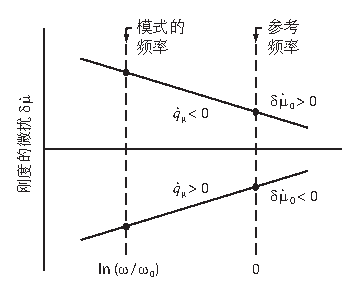
\includegraphics{../figures/chap13/fig01.eps}
\end{center}
\caption[lat het Q]{\label{13.fig.lathet}
\iffalse
If the aspherical
elastic and anelastic perturbations are due to lateral
variations in temperature, then high-rigidity
regions will exhibit less attenuation, and vice versa
(Karato \citeyear{karato93}).  The lateral variations
$\delta\hat{\mu}$ at the frequency $\omega$ of a mode ({\em left\/})
will in that case be more pronounced than the variations
$\delta\hat{\mu}_0$ at a higher reference frequency
$\omega_0$ ({\em right\/}).  The abscissa in this
schematic plot is the logarithm of frequency;
the perturbation in rigidity depends linearly upon
this variable: $\delta\hat{\mu}=\delta\hat{\mu}_0
+(2/\pi)\mu_0\hat{q}_{\mu}\ln(\omega/\omega_0)$.
\fi
若非球形弹性微扰和非弹性微扰是源于温度的横向变化所致,
则刚度较高的区域会表现出较小的衰减,反之亦然(Karato \citeyear{karato93})。
这种情况下,处于一模式频率$\omega$ (左)上的横向变化量$\delta\hat{\mu}$,
会比处在更高的参考频率$\omega_0$(右)的变化量$\delta\hat{\mu}_0$更加显著。
在这示意图中横轴是对数频率; 刚度微扰与此变量线性相依:
$\delta\hat{\mu}=\delta\hat{\mu}_0
+(2/\pi)\mu_0\hat{q}_{\mu}\ln(\omega/\omega_0)$。
}
\end{figure}
%It is straightforward to express the volumetric perturbations
%in terms of the P-wave and S-wave speed rather than the
%incompressibility and rigidity, using the first-order relations
我们很直观地利用以下的一阶关系式,以P波和S波波速,而非不可压缩性和刚度,来表示体积微扰
\eq
\delta\hspace{-0.1 mm}\kappa=\delta\hspace{-0.2 mm}\rho
\hspace{0.2 mm}(\alpha_0^2-\fourthirds\beta_0^2)+2\rho
(\alpha_0\,\delta\hspace{-0.1 mm}\alpha
-\fourthirds\beta_0\,\delta\hspace{-0.2 mm}\beta),
\en
\eq
\delta\hspace{-0.2 mm}\mu=\delta\hspace{-0.2 mm}\rho
\,\beta_0^2+2\rho\beta_0\,\delta\hspace{-0.2 mm}\beta,
\en
%where
其中 
$\alpha_0=[(\kappa_0+\fourthirds\mu_0)/_{\!}\rho]^{1/2}$
%and
和 
$\beta_0=(\mu_0/\!\rho)^{1/2}$。
%If we define reciprocal P-wave and S-wave quality factors by
假如我们定义P波和S波品质因子的倒数如下
\eq
q_{\alpha}=[1-\fourthirds(\beta_0/\hspace{-0.1 mm}\alpha_0)^2]q_{\kappa}
+\fourthirds(\beta_0/\hspace{-0.1 mm}\alpha_0)^2q_{\mu},\qquad
q_{\beta}=q_{\mu},
\en
%then it is easily demonstrated that
则很容易证明
\eq
\delta\hspace{-0.1 mm}\alpha=\delta\hspace{-0.1 mm}\bar{\alpha}
+\delta\hspace{-0.1 mm}\hat{\alpha},\qquad
\delta\hspace{-0.2 mm}\beta=\delta\hspace{-0.2 mm}\bar{\beta}
+\delta\hspace{-0.2 mm}\hat{\beta},
\en
%where
其中
\eq
\label{13.fancy5}
\delta\hspace{-0.1 mm}\bar{\alpha}=
\delta\hspace{-0.1 mm}\bar{\alpha}_0
+(1/\hspace{-0.2 mm}\pi)\alpha_0\bar{q}_{\alpha}\ln
(\omega/\omega_0),
\en
\eq
\delta\hspace{-0.1 mm}\hat{\alpha}=
\delta\hspace{-0.1 mm}\hat{\alpha}_0
+(1/\hspace{-0.2 mm}\pi)\alpha_0\hat{q}_{\alpha}\ln
(\omega/\omega_0),
\en
\eq
\delta\hspace{-0.2 mm}\bar{\beta}=
\delta\hspace{-0.2 mm}\bar{\beta}_0
+(1/\hspace{-0.2 mm}\pi)\beta_0\bar{q}_{\beta}\ln
(\omega/\omega_0),
\en
\eq
\label{13.fancy8}
\delta\hspace{-0.2 mm}\hat{\beta}=
\delta\hspace{-0.2 mm}\hat{\beta}_0
+(1/\hspace{-0.2 mm}\pi)\beta_0\hat{q}_{\beta}\ln
(\omega/\omega_0).
\en
%%%
\iffalse
The tendency for the percent lateral heterogeneity
to be accentuated at lower frequencies is more pronounced
for $\delta\hspace{-0.2 mm}\hat{\beta}/\hspace{-0.3 mm}\beta_0$
than for $\delta\hspace{-0.1 mm}\hat{\alpha}/\hspace{-0.1 mm}\alpha_0$
by a factor of $\hat{q}_{\beta}/\hat{q}_{\alpha}
\approx\threefourths(\alpha_0/\hspace{-0.3 mm}\beta_0)^2\approx\ninefourths$,
where the first approximation assumes
that $\hat{q}_{\kappa}\ll\hat{q}_{\mu}$,
and the final value is based upon the Poisson approximation.
\fi
%%%
$\delta\hspace{-0.2 mm}\hat{\beta}/\hspace{-0.3 mm}\beta_0$
在较低频率下横向不均匀性的程度加剧的趋势相较
$\delta\hspace{-0.1 mm}\hat{\alpha}/\hspace{-0.1 mm}\alpha_0$更为显著,
其比值为
$\hat{q}_{\beta}/\hat{q}_{\alpha}
\approx\threefourths(\alpha_0/\hspace{-0.3 mm}\beta_0)^2\approx\ninefourths$
\index{perturbation!anelastic|)}%,
其中第一个近似假设$\hat{q}_{\kappa}\ll\hat{q}_{\mu}$,而最后的值则是依据泊松近似。
%%%
\index{anelasticity|)}%


\renewcommand{\thesubsection}{$\!\!\!\raise1.3ex\hbox{$\star$}\!\!$
\arabic{chapter}.\arabic{section}.\arabic{subsection}}
%\subsection{Transverse isotropy}
\subsection{横向各向同性}
\index{perturbation!transversely isotropic|(}%
\index{transverse isotropy|(}%
\renewcommand{\thesubsection}{\arabic{chapter}.\arabic{section}.\arabic{subsection}}
\label{sec.13.ti}

%%%
\iffalse
Suppose now that the unperturbed spherical Earth is transversely isotropic
with elastic parameters $C_0$, $A_0$, $L_0$, $N_0$ and $F_0$, where the
subscript $0$ denotes evaluation at the reference frequency $\omega_0$.
The most general anelastic perturbation $\bdelta\bGamma(\om)$ now
consists of three parts:
\fi
%%%
现在假设未受扰动的球形地球是横向各向同性的,其弹性参数为$C_0$, $A_0$, $L_0$, $N_0$ 和 $F_0$, 
其中下标$0$表示在参考频率$\omega_0$的取值。
最一般的非弹性微扰$\bdelta\bGamma(\om)$现在由三个部分所组成:
%%%
\begin{enumerate}
\item 
%The incompressibility $\kappa_0=\ninth
%(C_0+4A_0-4N_0+4F_0)$ and the rigidity $\mu_0=\fifteenth(C_0
%+A_0+6L_0+5N_0-2F_0)$ exhibit three-dimensional
%perturbations of the form~(\ref{13.kappapert})--(\ref{13.mupert}).
不可压缩性$\kappa_0=\ninth (C_0+4A_0-4N_0+4F_0)$
和刚度$\mu_0=\fifteenth(C_0+A_0+6L_0+5N_0-2F_0)$ 
展现了~(\ref{13.kappapert})--(\ref{13.mupert})形式的三维微扰。
\item 
%In addition, the parameters
此外,表征横向各向同性的參數
$C_0^{\prime}=C_0-\kappa_0-\fourthirds\mu_0$,
$A_0^{\prime}=A_0-\kappa_0-\fourthirds\mu_0$,
$L_0^{\prime}=L_0-\mu_0$, $N_0^{\prime}=N_0-\mu_0$
%and
和 
$F_0^{\prime}=F_0-\kappa_0+\twothirds\mu_0$
%which characterize the transverse isotropy
%may undergo spherically symmetric perturbations
可能会经历球对称微扰
$\delta C_0^{\prime}$,
$\delta\hspace{-0.2 mm}A_0^{\prime}$,
$\delta\hspace{-0.2 mm}L_0^{\prime}$,
$\delta\hspace{-0.2 mm}N_0^{\prime}$ 
%and
和
$\delta\hspace{-0.2 mm}F_0^{\prime}$
%.
。
\item  
%Finally, there may be a general three-dimensional
%anisotropic perturbation, which we shall continue to
%denote by $\bgamma$.
最后可能还有一个一般的三维各向异性微扰,我们将继续使用$\bgamma$来表示。
\end{enumerate}
%%%
\iffalse
The perturbations $\delta\hspace{-0.1 mm}\kappa(\om)
+i\kappa_0q_{\kappa}$ and $\delta\hspace{-0.2 mm}
\mu(\om)+i\mu_0q_{\mu}$ to the ``equivalent'' isotropic
\index{equivalent isotropic parameter}%
parameters are complex and frequency dependent,
whereas both of the anisotropic perturbations
are assumed to be real and frequency independent.
The first-order eigenfrequency perturbation is still of the
form~(\ref{13.hydroHYDRO}), with the discontinuity kernels
replaced by
\fi
%%%
相对于“等价”的各向同性参数的微扰$\delta\hspace{-0.1 mm}\kappa(\om)
+i\kappa_0q_{\kappa}$ 和 $\delta\hspace{-0.2 mm}\mu(\om)+i\mu_0q_{\mu}$
是复数且频率相依的,
而它们的非弹性微扰则假设是实数且与频率无关。
一阶的本征频率微扰依然是~(\ref{13.hydroHYDRO})的形式,只不过不连续面的积分核由下式取代
%%%
\eqa
\label{13.HsphTI}
\lefteqn{2\omega K_{\rm d}=
\rho(\omega^2\bs\cdot\bs
-2\bs\cdot\bdel_{\!}\phi
-8\pi G\rho s_r^2-g\Upsilon)} \nonumber \\
&&\mbox{}+C_0(\p_rs_r)^2-(A_0-2N_0)(\bdel\cdot\bs-\p_rs_r)^2 \nonumber \\
&&\mbox{}\qquad-2N_0[\beps\!:\!\beps-2|\brh\cdot\beps|^2
+(\p_rs_r)^2] \nonumber \\
&&\mbox{}\qquad\qquad-4L_0(\brh\cdot\beps)\cdot(\brh\cdot\beps-\p_r\bs),
\ena
\eq
\label{13.KsphTI}
2\omega\bK_{\rm d}=-
2[C_0\p_rs_r+F_0(\bdel\cdot\bs-\p_rs_r)]\bs.
\en
%The spherically symmetric anisotropic perturbation
%may be accounted for by adding a term
球对称的各向异性微扰可以通过在三维对$\delta\omega$的表达式中加入一个项
$\int_0^a(\delta C_0^{\prime}\hspace{0.3 mm}K_C
+\delta\hspace{-0.2 mm}A_0^{\prime}\hspace{0.3 mm}K_A
+\delta\hspace{-0.2 mm}L_0^{\prime}\hspace{0.3 mm}K_L
+\delta\hspace{-0.2 mm}N_0^{\prime}\hspace{0.3 mm}K_N
+\delta\hspace{-0.2 mm}F_0^{\prime}\hspace{0.3 mm}K_F)\,dr$
%to the three-dimensional expression for $\delta\om$.
。
%The one-dimensional Fr\'{e}chet kernels 
一维的Fr\'{e}chet积分核
$K_C$,
$K_A$, $K_L$, $K_N$ and $K_F$ 
%are given in equations~(\ref{9.Ckern})--(\ref{9.Fkern}).
已定义在方程~(\ref{9.Ckern})--(\ref{9.Fkern})中。
%We shall eschew further consideration of transverse isotropy,
%and regard both the unperturbed spherical and perturbed
%aspherical Earth as isotropic throughout the remainder
%of this discussion.
我们将不再对横向各向同性做进一步考虑,并在剩余的讨论中将未受扰动的球形地球和非球形地球视为是各向同性的。
\index{perturbation!transversely isotropic|)}%
\index{transverse isotropy|)}%


\renewcommand{\thesubsection}{$\!\!\!\raise1.3ex\hbox{$\star$}\!\!$
\arabic{chapter}.\arabic{section}.\arabic{subsection}}
%\subsection{Rotation}
\subsection{旋转}
\index{rotation|(}%
\index{perturbation!rotational|(}%
\renewcommand{\thesubsection}{\arabic{chapter}.\arabic{section}.\arabic{subsection}}

%%%
\iffalse
The Coriolis force does not exert a first-order
influence upon the eigenfrequency
of a non-degenerate normal mode by virtue
\index{Coriolis force}%
\index{force!Coriolis}%
of the triple-product identity
$\bs\cdot(\bOmega\times\bs)=0$.
The effect of the centrifugal force, which is
of second order in the rotation rate
$\Omega=\|\bOmega\|$, can be accounted for by replacing
the  gravitational potential perturbation $\delta\Phi$
by $\delta\Phi+\psi$ in the volumetric kernel~(\ref{13.SphSTART}).
The centrifugal potential \vspace{-0.2 mm} $\psi$
has both a spherical part $\bar{\psi}$
and an aspherical part $\hat{\psi}$,
and the argument in Section~\ref{13.sec.SNREI}
regarding the determination of the
hydrostatic pressure and density perturbations
within the fluid regions of the Earth
must be modified by replacing $\delta\bar{\Phi}$
by $\delta\bar{\Phi}+\bar{\psi}$
in equation~(\ref{13.corepbar}) and $\delta\hat{\Phi}$
by $\delta\hat{\Phi}+\hat{\psi}$ in
equations~(\ref{13.corephat}),~(\ref{13.equipot})
and the right side of~(\ref{13.corePhibar}) for this reason.
The Coriolis force does act to split the degenerate
eigenfrequencies of isolated spherical-Earth multiplets
and to couple quasi-degenerate multiplets satisfying certain
selection rules.  These effects, which are much more
important than the effects of the centrifugal force,
inasmuch as they are of first order in $\Omega$,
are accounted for in Section~\ref{13.sec.couple}.
A more thorough discussion of the influence of the
rotation and associated hydrostatic ellipticity of
the Earth is given in Chapter~14.
\fi
%%%
由于三重积等式$\bs\cdot(\bOmega\times\bs)=0$,
科里奥利力不会对非简并简正模式的本征频率产生一阶项的影响。
而离心力的效应则为旋转速率$\Omega=\|\bOmega\|$的二阶量,
在体积积分核(~(\ref{13.SphSTART})中可用$\delta\Phi+\psi$置换引力势$\delta\Phi$来考虑此作用。 
离心势\vspace{-0.2 mm}$\psi$有球形部分$\bar{\psi}$,也有非球形部分$\hat{\psi}$。
为此,第~\ref{13.sec.SNREI}节中关于在地球液态区域的流体静压强和密度微扰的推导必须加以修改,
其中方程~(\ref{13.corepbar})中的$\delta\bar{\Phi}$须置换成$\delta\bar{\Phi}+\bar{\psi}$,
而方程~(\ref{13.corephat})、~(\ref{13.equipot})和~(\ref{13.corePhibar})的右侧中的
$\delta\hat{\Phi}$须被$\delta\hat{\Phi}+\hat{\psi}$取代。
科里奥利力确实会造成球对称地球孤立多态模式简并本征频率的分裂,
并将符合某些选择定理的准简并多态模式耦合起来。
有鉴于这些科里奥利力带来的影响相当于$\Omega$的一阶项,
因此远比离心力的作用更为重要,这将会在第~\ref{13.sec.couple}节中说明。
而对地球旋转和相关的流体静力学椭率的作用则将在第~14章做更全面的讨论。
%%%
\index{rotation|)}%
\index{perturbation!rotational|)}%


%\subsection{Perturbed kinetic and potential energy}
\subsection{微扰的动能和势能}
\index{energy!kinetic!perturbed|(}%
\index{energy!potential!perturbed|(}%
\index{perturbed kinetic energy|(}%
\index{kinetic energy!perturbed|(}%
\index{potential energy!perturbed|(}%
\index{perturbed potential energy|(}%

%%%
\iffalse
The final expression~(\ref{13.hydroHYDRO}) for the
eigenfrequency perturbation of a non-degenerate mode
can be ``derived'' in a purely symbolic manner by
taking the total variation of the energy equipartition
relation
\fi
%%%
对于非简并模式的本征频率微扰,其最终的表达式~(\ref{13.hydroHYDRO})
可以一个纯符号的方式,借由采取能量均分关系的总变分而推导出来:
%%%
\eq
\half(\om^2\sT-\sV)=0.
\en
%The variation with respect
%to the eigenfunction $\bs$ vanishes by virtue
%of Rayleigh's principle, leaving the first-order result
根据瑞利原理,与本征函数$\bs$有关的变分消失了,剩下一阶的结果
\eq 
\label{13.symbolic}
\delta\om=(2\om)^{-1}(\delta\sV-\om^2\delta\sT),
\en
%%%
\iffalse
where we have made use of the normalization relation
$\sT=1$.  The perturbations in the kinetic and potential
energies $\delta\sT$, $\delta\sV$ in equation~(\ref{13.symbolic})
are due strictly to the perturbations
$\delta\hspace{-0.1 mm}\kappa$, $\delta\hspace{-0.2 mm}\mu$,
$\delta\hspace{-0.2 mm}\rho$, $\delta\Phi$, $\delta\hspace{-0.1 mm}d$
and $\bgamma$ in the Earth model.
The perturbation in the kinetic energy functional
is given simply by
\fi
%%%
其中我们已使用了归一化关系$\sT=1$。
在方程~(\ref{13.symbolic})中动能和势能的微扰$\delta\sT$, $\delta\sV$
是严格地源于地球模型中的微扰$\delta\hspace{-0.1 mm}\kappa$, $\delta\hspace{-0.2 mm}\mu$,
$\delta\hspace{-0.2 mm}\rho$, $\delta\Phi$, $\delta\hspace{-0.1 mm}d$
和 $\bgamma$。
动能微扰的泛函可以简单地由下式给出
%%%
\eq
\label{13.kinener}
\delta\sT=\int_{\subearth}\delta\hspace{-0.2 mm}
\rho\hspace{0.3 mm}(\bs\cdot\bs)\,dV
-\int_{\Sigma}\delta\hspace{-0.1 mm}d\hspace{0.3 mm}
[\rho\,\bs\cdot\bs]^+_-\,d\/\Sigma,
\en
%%%
\iffalse
where the surface integral accounts for the change in the region
of integration.  Upon comparing the results~(\ref{13.hydroHYDRO})
and~(\ref{13.symbolic}) and extracting the expression~(\ref{13.kinener})
from equations~(\ref{13.SphSTART})--(\ref{13.KsphSTART}), we infer that
the corresponding perturbation in the elastic-gravitational
potential-energy functional is
\fi
%%%
其中的面积分说明了积分区域的改变。
通过比较~(\ref{13.hydroHYDRO})和~(\ref{13.symbolic})的结果,
并从方程~(\ref{13.SphSTART})--(\ref{13.KsphSTART})提取表达式~(\ref{13.kinener}),
我们推导出相应的弹性-重力势能泛函微扰为
%%%
\eqa
\label{13.potener}
\lefteqn{\delta\sV=\int_{\subearth}
[\delta\hspace{-0.1 mm}\kappa(\bdel\cdot\bs)^2
+2\hspace{0.2 mm}\delta\hspace{-0.2 mm}\mu(\bd\!:\!\bd)
+\delta\hspace{-0.2 mm}\rho\hspace{0.3 mm}
(2\bs\cdot\bdel_{\!}\phi+4\pi G\rho s_r^2+g\Upsilon)} \nonumber \\
&&\mbox{}\quad+\rho\bdel(\delta\Phi)\cdot(\bs\cdot\bdel\bs
-\bs\bdel\cdot\bs)+\rho\hspace{0.3 mm}\bs\cdot\bdel\bdel(\delta\Phi)\cdot\bs
+\beps\!:\!\bgamma\!:\!\beps]\,dV \nonumber \\
&&\mbox{}\!\!\!\!\!-\int_{\Sigma}\delta\hspace{-0.1 mm}d_{\,}
[\kappa_0(\bdel\cdot\bs)(\bdel\cdot\bs-2\p_rs_r)
+2\mu_0\bd\!:\!(\bd-2\brh\p_r\bs) \nonumber \\
&&\mbox{}\quad+\rho(2\bs\cdot\bdel_{\!}\phi
+8\pi G\rho s_r^2+g\Upsilon)]^+_-\,d\/\Sigma \nonumber \\
&&\mbox{}\!\!\!\!\!-\int_{\Sigma_{\rm FS}}\bdel^{\Sigma}
(\delta\hspace{-0.1 mm}d)\cdot
[2\kappa_0(\bdel\cdot\bs)\bs+4\mu_0d_{rr}\bs]^+_-\,d\/\Sigma.
\ena
%%%
\iffalse
The perturbations $\delta\hspace{-0.1 mm}\kappa$ and
$\delta\hspace{-0.2 mm}\mu$ in equation~(\ref{13.potener})
are those ``seen'' by the mode of frequency $\omega$.
This decomposition of the eigenfrequency perturbation
$\delta\om$ into separate kinetic and potential
energy perturbations $\delta\sT$ and $\delta\sV$
provides a convenient starting point for extending
the above results to the case of actual seismological
interest, as we shall see next.
\fi
%%%
式~(\ref{13.potener})中$\delta\hspace{-0.1 mm}\kappa$和
$\delta\hspace{-0.2 mm}\mu$
是频率为$\omega$的模式所看到的微扰。
上述将本征频率微扰$\delta\omega$分解成单独的动能微扰$\delta\sT$和势能微扰$\delta\sV$的做法,
为扩展至实际地震学的情况提供了一个方便的起点,而我们将会在接下来的章节中看到。
%%%
\index{energy!kinetic!perturbed|)}%
\index{energy!potential!perturbed|)}%
\index{perturbed kinetic energy|)}%
\index{kinetic energy!perturbed|)}%
\index{potential energy!perturbed|)}%
\index{perturbed potential energy|)}%
\index{mode!isolated|)}%
\index{isolated mode|)}%


%\section{Degeneracy and Quasi-Degeneracy}
\section{简并和准简并}
\index{degeneracy|(}%
\index{eigenfrequency degeneracy|(}%
\index{quasi-degeneracy|(}%
\index{mode coupling|(}%
\index{mode!coupled|(}%
\index{coupled mode|(}%
\label{13.sec.couple}

%%%
\iffalse
Thus far we have treated the unperturbed eigenfrequencies
as if they were non-degenerate and well isolated in the
Earth's normal-mode spectrum.  In fact, the real eigenfrequencies
of a non-rotating, spherically symmetric Earth model occur in
$(2l+1)$-degenerate
toroidal and spheroidal multiplets ${}_n{\rm T}_l$
and ${}_n{\rm S}_l$.
The three-dimensional
character of the structural
perturbations $\delta\hspace{-0.1 mm}\kappa$, $\delta\hspace{-0.2 mm}\mu$,
$\delta\hspace{-0.2 mm}\rho$, $\delta\Phi$, $\delta\hspace{-0.1 mm}d$
and $\bgamma$ and the
rotation of the Earth break
the spherical symmetry and remove
this eigenfrequency degeneracy.
Multiplets whose unperturbed eigenfrequencies
are in close juxtaposition may also be coupled
by rotation and any three-dimensional perturbations.
The simplest means of accounting for this
{\em eigenfrequency splitting\/} and
{\em quasi-degenerate mode coupling\/}
is to employ a modified version of the
Rayleigh-Ritz variational method discussed in
Chapter~7.  We use the real unperturbed {\em singlet\/} eigenfunctions
\index{singlet}%
$\bs_k$ associated with the multiplets whose coupling
we wish to investigate as the basis functions, and seek
perturbed singlet eigenfunctions 
of the form
\fi
%%%
迄今为止,我们把未受扰动的本征频率视为仿佛是非简并的,以及在地球简正模式频谱中十分孤立的模式。 
然而事实上,无旋、球对称地球模型的实数本征频率仅出现在
$(21+l)$-简并的环形多态模式${}_n{\rm T}_l$和球形多态模式${}_n{\rm S}_l$上。
结构微扰$\delta\hspace{-0.1 mm}\kappa$, $\delta\hspace{-0.2 mm}\mu$,
$\delta\hspace{-0.2 mm}\rho$, $\delta\Phi$, $\delta\hspace{-0.1 mm}d$
和 $\bgamma$的三维特征
以及地球的旋转打破了球对称性,且消除了本征频率的简并。
在未受扰动的本征频率上,相邻的数个多态模式也可能会因为旋转和任何三维的微扰而耦合。
解释此种本征频率分裂和准简并模式耦合的最简单方法是采用第七章中所讨论的修正版的瑞利-里兹变分法。
我们利用实数、未受扰动的单态模式本征函数$\bs_k$
\index{singlet}%
作为基函数,
与此单态模式本征函数相关的多态模式之耦合正是我们希望探究的,
因此我们进一步寻找受扰动的单态模式本征函数的形式
\eq \label{13.Rayexp}
\bs=\sum_kq_k\bs_k,
\en
%%%
\iffalse
where the expansion coefficients $q_k$ must be determined.
In principle, we should incorporate all of the
unperturbed eigenfunctions in the basis set;
in practice, of course, we must restrict consideration
to a finite number of quasi-degenerate multiplets.
\fi
%%%
其中展开系数必须被决定。
原则上我们应将所有未受扰动的本征函数都纳入基集;
但实际上则必须将准简并多态模式限制在有限的数量。
%%%

%%%
\iffalse
We treat the split singlet eigenfrequencies as small
perturbations away from a positive reference or fiducial
frequency $\om_0$; all significant coupling partners ${}_n{\rm T}_l$
and ${}_n{\rm S}_l$ with degenerate eigenfrequencies
$\om_k$ in the vicinity of the reference frequency
$\om_0$ are presumed to be included in the
spherical-Earth basis set.  The orthonormality
$\int_{\subearth}\rho\hspace{0.2 mm}\bs_k\cdot\bs_{k'}\,dV=\delta_{kk'}$
of the basis eigenfunctions guarantees that the unperturbed
kinetic energy matrix is simply the identity $\ssI$,
whereas the unperturbed elastic-gravitational potential energy
matrix is the diagonal matrix
$\ssOmega^2={\rm diag}\,[\cdots\,\om_k^2\,\cdots]$
of squared degenerate eigenfrequencies.
Note that each squared eigenfrequency is repeated
$2l+1$ times along the diagonal;
the index $k$ does ``double duty'' as a label
of both basis eigenfunctions $\bs_k$ and associated unperturbed
eigenfrequencies $\om_k$.
\fi
%%%
我们将分裂的单态模式本征频率视为偏离正的参考或基准频率$\omega_0$的微扰;
所有在参考频率$\omega_0$附近具有简并本征频率$\omega_k$的重要的耦合组合${}_n{\rm T}_l$
和 ${}_n{\rm S}_l$
都被假定包含在球形地球的基集中。
本征基函数(basis eigenfunction)的正交归一性$\int_{\subearth}\rho\hspace{0.2 mm}\bs_k\cdot\bs_{k'}\,dV=\delta_{kk'}$
确保了未受扰动的张量为一简单的单位张量~$\ssI$,
而未受扰动的弹性-重力势能矩阵是简并本征频率平方的对角矩阵
$\ssOmega^2={\rm diag}\,[\cdots\,\om_k^2\,\cdots]$。
请注意,每个本征频率的平方沿对角线重复了$2l+1$次;
角标$k$有作为本征基函数和相关的未受扰动本征频率$\omega_k$的标签之双重作用。
%%%
\iffalse
Notable contributions to the theory of quasi-degenerate
multiplet coupling have been made by \textcite{dahlen69},
\textcite{luh73}, \textcite{woodhouse80} and
\textcite{park&gilbert86}; we summarize and extend
these original treatments here.  The most significant
new feature in the following development
is a renormalization procedure which yields
singlet eigenfunctions~(\ref{13.Rayexp}) that are
correctly orthonormalized or biorthonormalized in accordance with the
fundamental principles enunciated in Chapters 4 and 6.  We consider
the simplest situation---a non-rotating, perfectly
elastic perturbation---before dealing with the
complications introduced by rotation and anelasticity,
first in isolation and then in tandem.
\fi
\textcite{dahlen69},
\textcite{luh73}, \textcite{woodhouse80} 和
\textcite{park&gilbert86}
对准简并多态模式耦合理论做出了重要的贡献;
我们在此总结并扩展这些原始的处理。
而在后续的发展中,最重要且新的方面是重归一化的步骤。
该步骤得到的单态模式本征函数~(\ref{13.Rayexp})被正确地正交归一化或双正交归一化,
这与在第4章和第6章中阐述的基本原理相符。
在处理旋转和非弹性所带来的复杂情况之前,我们先考虑最简单的情况---无旋纯弹性微扰---将这些情况先单独分开考虑,然后再合并一起讨论。
%%%

%\subsection{Non-rotating elastic perturbation}
\subsection{无旋弹性微扰}
\index{perturbation!non-rotating elastic|(}%
\index{Rayleigh-Ritz method!non-rotating Earth|(}%

%%%
\iffalse
The kinetic and potential energy matrices
$\ssI$ and $\ssOmega^2$ are altered
as a result of the perturbations $\delta\hspace{-0.1 mm}\kappa$,
$\delta\hspace{-0.2 mm}\mu$,
$\delta\hspace{-0.2 mm}\rho$, $\delta\Phi$, $\delta\hspace{-0.1 mm}d$
and $\bgamma$ in the Earth model.
Adopting a slightly modified version of the notation
employed in Chapter 7, we shall henceforth use $\ssT$
and $\ssV$ to denote the {\em first-order perturbation matrices\/}.
\index{perturbation matrix}%
\index{matrix!perturbation}%
The elements $T_{kk'}$ and $V_{kk'}$ of these matrices are symmetrized
generalizations of the expressions~(\ref{13.kinener})
and~(\ref{13.potener}) for the perturbed
scalar kinetic and potential
energy of a non-degenerate mode:
\fi
%%%
由于地球模型中的微扰
$\delta\hspace{-0.1 mm}\kappa$,
$\delta\hspace{-0.2 mm}\mu$,
$\delta\hspace{-0.2 mm}\rho$, $\delta\Phi$, $\delta\hspace{-0.1 mm}d$
和$\bgamma$,
改变了动能矩阵$\ssI$和势能矩阵$\ssOmega^2$。
我们采用了在第七章所使用的稍加修正版本的符号,
在之后用$\ssT$和$\ssV$来表示一阶的微扰矩阵。
\index{perturbation matrix}%
\index{matrix!perturbation}%
这些矩阵的元素 $T_{kk'}$和$V_{kk'}$是对一非简并模式的微扰标量动能~(\ref{13.kinener})
和微扰标量势能~(\ref{13.potener})的表达式,将其对称化的一般式:
%%%
\eq \label{13.delTdef}
T_{kk'}=\int_{\subearth}\delta\hspace{-0.2 mm}
\rho\hspace{0.3 mm}(\bs_k\cdot\bs_{k'})\,dV
-\int_{\Sigma}\delta\hspace{-0.1 mm}d
\,[\rho\,\bs_k\cdot\bs_{k'}]^+_-\,d\/\Sigma,
\en
\eqa
\label{13.delVdef}
\lefteqn{V_{kk'}=\int_{\subearth}
[\delta\hspace{-0.1 mm}\kappa(\bdel\cdot\bs_k)
(\bdel\cdot\bs_{k'})+2\hspace{0.2 mm}\delta\hspace{-0.2 mm}\mu
(\bd_k\!:\!\bd_{k'})} \nonumber \\
&&\mbox{}\qquad+\delta\hspace{-0.2 mm}\rho
\hspace{0.3 mm}\{\bs_k\cdot\bdel_{\!}\phi_{k'}
+\bs_{k'}\cdot\bdel_{\!}\phi_k \nonumber \\
&&\mbox{}\qquad+4\pi G\rho(\brh\cdot\bs_k)
(\brh\cdot\bs_{k'})+g\Upsilon_{kk'}\} \nonumber \\
&&\mbox{}\qquad+\half\rho\bdel(\delta\Phi)\cdot(\bs_k\cdot\!\bdel\bs_{k'}
+\bs_{k'}\cdot\!\bdel\bs_k \nonumber \\
&&\mbox{}\qquad-\bs_k\bdel\cdot\bs_{k'}
-\bs_{k'}\bdel\cdot\bs_k)
+\rho\hspace{0.3 mm}\bs_k\cdot\bdel\bdel(\delta\Phi)\cdot\bs_{k'} \nonumber \\
&&\mbox{}\qquad+\beps_k\!:\!\bgamma\!:\!\beps_{k'}]\,dV \nonumber \\
&&\mbox{}\,-\int_{\Sigma}\delta\hspace{-0.1 mm}d_{\,}
[\half\kappa(\bdel\cdot\bs_k)(\bdel\cdot\bs_{k'}-2\brh\cdot\p_r\bs_{k'}) \nonumber \\
&&\mbox{}\qquad
+\half\kappa(\bdel\cdot\bs_{k'})(\bdel\cdot\bs_k-2\brh\cdot\p_r\bs_k) \nonumber \\
&&\mbox{}\qquad+\mu\bd_k\!:\!(\bd_{k'}-2\brh\p_r\bs_{k'})
+\mu\bd_{k'}\!:\!(\bd_k-2\brh\p_r\bs_k) \nonumber \\
&&\mbox{}\qquad+\rho\hspace{0.3 mm}\{\bs_k\cdot\bdel_{\!}\phi_{k'}
+\bs_{k'}\cdot\bdel_{\!}\phi_k \nonumber \\
&&\mbox{}\qquad+8\pi G\rho(\brh\cdot\bs_k)
(\brh\cdot\bs_{k'})+g\Upsilon_{kk'}\}]^+_-\,d\/\Sigma \nonumber \\
&&\mbox{}\,-\int_{\Sigma_{\rm FS}}\bdel^{\Sigma}
(\delta\hspace{-0.1 mm}d)\cdot
[\kappa(\bdel\cdot\bs_k)\bs_{k'}+\kappa(\bdel\cdot\bs_{k'})\bs_k \nonumber \\
&&\mbox{}\qquad
+2\mu(\brh\cdot\bd_k\cdot\brh)\bs_{k'}
+2\mu(\brh\cdot\bd_{k'}\cdot\brh)\bs_k]^+_-\,d\/\Sigma,
\ena
%where
其中
\eqa \label{13.newUpsdef} \lefteqn{
\Upsilon_{kk'}=\half[\bs_k\cdot\bdel(\brh\cdot\bs_{k'})
+\bs_{k'}\cdot\bdel(\brh\cdot\bs_k)]} \nonumber \\
&&\mbox{}\qquad-\half[(\brh\cdot\bs_k)(\bdel\cdot\bs_{k'})
+(\brh\cdot\bs_{k'})(\bdel\cdot\bs_k)] \nonumber \\
&&\mbox{}\qquad\qquad-2r^{-1}(\brh\cdot\bs_k)(\brh\cdot\bs_{k'}).
\ena
%The reality of
%the unperturbed eigenfunctions $\bs_k$ guarantees
%that both of the perturbation matrices
%are real and symmetric: $\ssT^{\rm T}\!=\ssT$ and
%$\ssV^{\rm T}\!=\ssV$, where the
%superscript T denotes the transpose.
实数的未受扰动本征函数$\bs_k$确保了这两个微扰矩阵皆为实数和对称:
$\ssT^{\rm T}\!=\ssT$ 和 $\ssV^{\rm T}\!=\ssV$,
其中上标T表示转置。

%The perturbed eigenfrequencies of the singlets in the vicinity
%of the reference frequency $\om_0$ will be expressed in the form
在参考频率$\om_0$附近,受扰动的单态模式本征频率以下列形式表示
\eq
\om=\om_0+\delta\om,
\en

%%%
\iffalse
where it is assumed that $|\delta\om|\ll\om_0$.  To determine the
perturbations $\delta\om$ and the associated column
vectors $\ssq$ of eigenfunction expansion coefficients $q_k$,
we must solve the generalized eigenvalue
problem~(\ref{7.VqTq}).  Rewritten in the present
notation, this equation takes the form
\fi
%%%
其中假设$|\delta\om|\ll\om_0$。
为了决定微扰$\delta\om$以及相关的本征函数展开系数$q_k$之列矢量$\ssq$,
我们必须求解广义本征值问题~(\ref{7.VqTq})。
使用当前的表示符号重新改写此方程,得到了
%%%
\eq \label{13.VqTq}
(\ssOmega^2+\ssV)\ssq=(\om_0+\delta\om)^2
(\ssI+\ssT)\ssq.
\en
%We can reduce~(\ref{13.VqTq}) to an ordinary eigenvalue
%problem for the singlet eigenfrequency perturbations
%$\delta\om$ by defining the {\em renormalized 
%eigenvectors\/}
%\index{eigenvector!renormalized}%
%\index{renormalized eigenvector}%
%\eq \label{13.zdef}
%\ssz=(\ssI+\half\ssT)\ssq.
%\en
我们可通过定义重归一化的本征矢量
\index{eigenvector!renormalized}%
\index{renormalized eigenvector}%
\eq \label{13.zdef}
\ssz=(\ssI+\half\ssT)\ssq.
\en
%Upon inserting the representation~(\ref{13.zdef}) into
%equation~(\ref{13.VqTq}) and neglecting terms of second
%order in $\delta\om$, $\om_k-\om_0$, $\ssT$ and $\ssV$,
%we obtain
将~(\ref{13.VqTq})简化为一个对单态模式本征频率微扰$\delta\omega$的普通本征值问题。
接着将表达式~(\ref{13.zdef})带入方程~(\ref{13.VqTq})中,并忽略在
$\delta\om$, $\om_k-\om_0$, $\ssT$ 和 $\ssV$中的二阶项,可得到
\eq \label{13.Kq}
\ssH\ssz=\delta\om\,\ssz,
\en
%where
其中
\eq \label{13.Kdef}
\ssH=\ssOmega-\om_0\ssI+(2\om_0)^{-1}
(\ssV-\om_0^2\ssT).
\en
%%%
\iffalse
Since $\ssH$ is real and symmetric, $\ssH^{\rm T}\!=\ssH$,
its eigenvalues $\delta\om$ are real and its eigenvectors
are mutually orthogonal in the sense $\ssz^{\rm T}\ssz'=0$
if $\delta\om\neq\delta\om'$.  If we normalize the eigenvectors
by requiring that $\ssz^{\rm T}\ssz=1$,
then they constitute an {\em orthonormal basis\/}:
\fi
%%%
由于$\ssH$是实数且对称的$\ssH^{\rm T}\!=\ssH$,
因此它的本征值$\delta\omega$是实数,而它的本征矢量在这个意义上是相互正交的,
即$\ssz^{\rm T}\ssz'=0$,假若$\delta\om\neq\delta\om’$。
如果我们要求以$\ssz^{\rm T}\ssz=1$归一化本征矢量,
则它们就构成了一正交归一基(orthonormal basis):
\index{orthonormal basis}%
\index{basis!orthonormal}%
\eq \label{13.ZZeqI}
\ssZ^{\rm T}\ssZ=\ssI,
\en
%where $\ssZ$ is the square matrix whose columns are the
%renormalized eigenvectors $\ssz$.  We can rewrite the eigenvalue
%problem~(\ref{13.Kq}) in the form
其中$\ssZ$是方形矩阵,它的列是重归一化的本征矢量$\ssz$。
我们可以以下列形式改写此本征值问题~(\ref{13.Kq})
\eq \label{13.Kdiag}
\ssZ^{\rm T}\ssH\ssZ=\ssDelta,
\en
%%%
\iffalse
where $\ssDelta={\rm diag}\,[\cdots\,\delta\om\,\cdots]$
is the diagonal matrix of eigenfrequency perturbations.
Taken together, equations~(\ref{13.ZZeqI})--(\ref{13.Kdiag})
show that $\ssZ$ is the orthogonal matrix that diagonalizes
the {\em renormalized eigenfrequency perturbation matrix\/}
\index{perturbation matrix!renormalized}%
\index{matrix!perturbation}%
$\ssH$.  Correct to first order in $\ssT$, we may rewrite the
orthonormality relation~(\ref{13.ZZeqI}) in the form
\eq \label{13.QQeqI}
\ssQ^{\rm T}(\ssI+\ssT)\ssQ=\ssI,
\en
where $\ssQ$ is the square matrix of original column
vectors $\ssq$.
\fi
%%%
其中 $\ssDelta={\rm diag}\,[\cdots\,\delta\om\,\cdots]$是本征频率微扰的对角矩阵。
综合以上所述,
方程~(\ref{13.ZZeqI})--(\ref{13.Kdiag})表示Z是一个可以对
重归一化本征频率微扰矩阵$\ssH$
进行对角化的正交矩阵。
正确至$\ssT$的一阶量,我们可以将正交归一化关系~(\ref{13.ZZeqI})改写为
\eq \label{13.QQeqI}
\ssQ^{\rm T}(\ssI+\ssT)\ssQ=\ssI,
\en
其中$\ssQ$是由原来的列矢量$\ssq$所组成的方阵。
%%%

%%%
\iffalse
In summary, we can find the first-order singlet eigenfrequency
perturbations $\delta\om$ and associated renormalized
eigenvectors $\ssz$ of a non-rotating elastic Earth
by solving the real symmetric
eigenvalue problem $\ssH\ssz=\delta\om\,\ssz$
subject to the requirement that $\ssz^{\rm T}\ssz=1$.
The original eigenvectors $\ssq$ are given
in terms of the renormalized eigenvectors $\ssz$
by the inverse of equation~(\ref{13.zdef}):
\fi
%%%
总而言之,
我们可借由求解实数且对称的本征值问题$\ssH\ssz=\delta\om\,\ssz$,同时要求满足$\ssz^{\rm T}\ssz=1$,
找到在无旋弹性地球中单态模式的一阶本征频率微扰$\delta\omega$和与其相关的重归一化本征矢量$\ssz$。
取方程~(\ref{13.zdef})的逆,使原本的本征矢量$\ssq$以重归一化的本征矢量$\ssz$的形式表达为:
\eq \label{13.zrelq}
\ssq=(\ssI-\half\ssT)\ssz.
\en
%This two-step procedure
%for determining the singlet eigenfunctions~(\ref{13.Rayexp})
%renders them properly {\em orthonormal with
%respect to the perturbed Earth\/}, in the first-order sense
此两步骤求解单态模式本征矢量~(\ref{13.Rayexp})的过程,使得这些矢量对于受扰动的地球
在一阶意义上来说满足适当地正交,即
\eq \label{13.norm1}
\int_{\subearth}
(\rho+\delta\hspace{-0.2 mm}\rho)\,\bs\cdot\bs'\,dV
-\int_{\Sigma}\delta\hspace{-0.1 mm}d
\,[\rho\,\bs\cdot\bs']^+_-\,d\/\Sigma=0
\quad\mbox{若 $\delta\om\neq\delta\om'$,}
\en
\eq \label{13.norm2}
\int_{\subearth}
(\rho+\delta\hspace{-0.2 mm}\rho)\,\bs\cdot\bs\,dV
-\int_{\Sigma}\delta\hspace{-0.1 mm}d
\,[\rho\,\bs\cdot\bs]^+_-\,d\/\Sigma=1.
\en
%The three-dimensional equations~(\ref{13.norm1})--(\ref{13.norm2})
%are equivalent to the matrix orthonormality relation~(\ref{13.QQeqI}).
%The surface-integral terms account for the change in the
%domain of integration due to the boundary perturbations
%$\delta\hspace{-0.1 mm}d$.
上述两个三维方程~(\ref{13.norm1})--(\ref{13.norm2})等价于矩阵正交归一关系式~(\ref{13.QQeqI})。
面积分项反映了由边界微扰$\delta\hspace{-0.1 mm}d$所引起的积分域的变化。
\index{perturbation!non-rotating elastic|)}%
\index{Rayleigh-Ritz method!non-rotating Earth|)}%

\renewcommand{\thesubsection}{$\!\!\!\raise1.3ex\hbox{$\star$}\!\!$
\arabic{chapter}.\arabic{section}.\arabic{subsection}}
%\subsection{Rotating elastic perturbation}
\subsection{旋转弹性微扰}
\index{perturbation!rotating elastic|(}%
\index{Rayleigh-Ritz method!rotating Earth|(}%
\renewcommand{\thesubsection}{\arabic{chapter}.\arabic{section}.\arabic{subsection}}
\label{sec:13.2.2}

%%%
\iffalse
The effect of the centrifugal potential $\psi$ can be accounted for
by making the substitution $\delta\Phi\rightarrow\delta\Phi+\psi$
in equation~(\ref{13.delVdef}), as discussed in Section 13.1.11.
The perturbed kinetic energy matrix $\ssT$ is unchanged,
whereas the elements of the perturbed potential energy matrix
$\ssV$ are replaced by
\fi
%%%
离心势$\psi$的影响可以借由方程~(\ref{13.delVdef})中
$\delta\Phi\rightarrow\delta\Phi+\psi$的替换而被考虑,如同在第13.1.11节中的讨论。
微扰$\ssT$不变,然而微扰势能矩阵$\ssV$的元素则被置换为
%%%
\eqa
\label{13.delVdef2}
\lefteqn{V_{kk'}=\int_{\subearth}
[\delta\hspace{-0.1 mm}\kappa(\bdel\cdot\bs_k)
(\bdel\cdot\bs_{k'})+2\hspace{0.2 mm}\delta\hspace{-0.2 mm}\mu
(\bd_k\!:\!\bd_{k'})} \nonumber \\
&&\mbox{}\qquad+\delta\hspace{-0.2 mm}\rho\hspace{0.3 mm}
\{\bs_k\cdot\bdel_{\!}\phi_{k'}+\bs_{k'}\cdot\bdel_{\!}\phi_k \nonumber \\
&&\mbox{}\qquad+4\pi G\rho(\brh\cdot\bs_k)
(\brh\cdot\bs_{k'})+g\Upsilon_{kk'}\} \nonumber \\
&&\mbox{}\qquad+\half\rho\bdel(\delta\Phi+\psi)\cdot(\bs_k\cdot\!\bdel\bs_{k'}
+\bs_{k'}\cdot\!\bdel\bs_k \nonumber \\
&&\mbox{}\qquad-\bs_k\bdel\cdot\bs_{k'}
-\bs_{k'}\bdel\cdot\bs_k)
+\rho\bs_k\cdot\bdel\bdel(\delta\Phi+\psi)\cdot\bs_{k'} \nonumber \\
&&\mbox{}\qquad+\beps_k\!:\!\bgamma\!:\!\beps_{k'}]\,dV \nonumber \\
&&\mbox{}\,-\int_{\Sigma}\delta\hspace{-0.1 mm}d_{\,}
[\half\kappa(\bdel\cdot\bs_k)(\bdel\cdot\bs_{k'}-2\brh\cdot\p_r\bs_{k'}) \nonumber \\
&&\mbox{}\qquad
+\half\kappa(\bdel\cdot\bs_{k'})(\bdel\cdot\bs_k-2\brh\cdot\p_r\bs_k) \nonumber \\
&&\mbox{}\qquad+\mu\bd_k\!:\!(\bd_{k'}-2\brh\p_r\bs_{k'})
+\mu\bd_{k'}\!:\!(\bd_k-2\brh\p_r\bs_k) \nonumber \\
&&\mbox{}\qquad+\rho\hspace{0.3 mm}\{\bs_k\cdot\bdel_{\!}\phi_{k'}
+\bs_{k'}\cdot\bdel_{\!}\phi_k \nonumber \\
&&\mbox{}\qquad+8\pi G\rho(\brh\cdot\bs_k)
(\brh\cdot\bs_{k'})+g\Upsilon_{kk'}\}]^+_-\,d\/\Sigma \nonumber \\
&&\mbox{}\,-\int_{\Sigma_{\rm FS}}\bdel^{\Sigma}
(\delta\hspace{-0.1 mm}d)\cdot
[\kappa(\bdel\cdot\bs_k)\bs_{k'}+\kappa(\bdel\cdot\bs_{k'})\bs_k \nonumber \\
&&\mbox{}\qquad
+2\mu(\brh\cdot\bd_k\cdot\brh)\bs_{k'}
+2\mu(\brh\cdot\bd_{k'}\cdot\brh)\bs_k]^+_-\,d\/\Sigma.
\ena
%As in Chapter~7, where the Rayleigh-Ritz method was
%applied to an arbitrarily heterogeneous Earth,
%we also introduce the {\em Coriolis matrix\/}
%\index{Coriolis matrix}%
%\index{matrix!Coriolis}%
%$\ssW$ with elements
如同第7章中瑞利-里兹法应用于任意不均匀性的地球,
我们也引入了科里奥利矩阵$\ssW$,
\index{Coriolis matrix}%
\index{matrix!Coriolis}%
其元素为
\eq \label{13.Coriolis}
W_{kk'}=\int_{\subearth}\rho\hspace{0.3 mm}\bs_k\cdot(i\bOmega\times\bs_{k'})\,dV.
\en
%%%
\iffalse
Both $\ssT$ and $\ssV$ are still real and symmetric,
whereas the Coriolis matrix $\ssW$ is imaginary and anti-symmetric.
All three perturbation matrices, if regarded as complex, are therefore Hermitian:
$\ssT^{\rm H}=\ssT$, $\ssV^{\rm H}=\ssV$ and $\ssW^{\rm H}=\ssW$,
where the superscript H denotes the complex conjugate transpose.
The non-standard generalized eigenvalue problem~(\ref{7.VqTqrot})
governing the normal modes of a rotating elastic Earth is
\fi
%%%
$\ssT$和$\ssV$两者仍是实数且对称的,然而科里奥利矩阵$\ssW$则是虚数且反对称的。
因此若将这三个微扰矩阵视作复数,则其具有厄米特性:
$\ssT^{\rm H}=\ssT$, $\ssV^{\rm H}=\ssV$ 和 $\ssW^{\rm H}=\ssW$,
其中上标H表示复数共轭转置。
控制有旋弹性地球简正模式的非标准广义本征值问题~(\ref{7.VqTqrot})为
%%%
\eq \label{13.VqTqrot}
[\ssOmega^2+\ssV+2(\om_0+\delta\om)\ssW-(\om_0+\delta\om)^2
(\ssI+\ssT)]\hspace{0.2 mm}\ssq=\sszero.
\en
%%%
\iffalse
Generalizing~(\ref{13.zdef}), we account for the effect of
the Coriolis force by defining the renormalized eigenvectors
\eq \label{13.zdef2}
\ssz=(\ssI+\half\ssT-\half\om_0^{-1}\ssW)\ssq.
\en
Upon inserting equation~(\ref{13.zdef2})
into~(\ref{13.VqTqrot}) and neglecting terms
that are of second order in $\delta\om$,
$\om_k-\om_0$, $\ssT$, $\ssV$ and $\ssW$,
we obtain an ordinary eigenvalue problem
analogous to~(\ref{13.Kq}):
\fi
%%%
为了将式子~(\ref{13.zdef})一般化,我们通过定义重归一化的本征矢量
\eq \label{13.zdef2}
\ssz=(\ssI+\half\ssT-\half\om_0^{-1}\ssW)\ssq,
\en
来考虑科里奥利力的影响。
将方程~(\ref{13.zdef2})代入~(\ref{13.VqTqrot}),并忽略
$\delta\om$, $\om_k-\om_0$, $\ssT$, $\ssV$ 和 $\ssW$ 的二阶项,
我们获得了一个类似~(\ref{13.Kq})的普通本征值问题: 
%%%
\eq \label{13.Kq2}
\ssH\ssz=\delta\om\,\ssz,
\en
%where
其中
\eq \label{13.Kdef2}
\ssH=\ssOmega-\om_0\ssI+\ssW+(2\om_0)^{-1}
(\ssV-\om_0^2\ssT).
\en
%The Hermitian symmetry $\ssH^{\rm H}\!=\ssH$ of the complex
%renormalized eigenfrequency perturbation matrix~(\ref{13.Kdef2})
%guarantees that all of the eigenfrequency perturbations
%$\delta\om$ are real, and that the associated eigenvectors $\ssz$
%may be orthonormalized in the sense
此复数重归一化本征频率微扰矩阵~(\ref{13.Kdef2})的厄米特对称性$\ssH^{\rm H}\!=\ssH$,
确保了所有的本征频率微扰$\delta\omega$皆为实数,且相关的本征矢量$\ssz$可被正交归一化,即
\eq \label{13.KKeqI2}
\ssZ^{\rm H}\ssZ=\ssI.
\en
%We can rewrite the
%eigenvalue problem~(\ref{13.Kq2}) in terms of
%the matrix of complex eigenvectors
%$\ssZ$ and the diagonal matrix of real eigenfrequency
%perturbations $\ssDelta={\rm diag}\,[\cdots\,\delta\om\,\cdots]$
%in a form analogous to equation~(\ref{13.Kdiag}):
我们可利用复数的本征矢量矩阵$\ssZ$和实数的本征频率微扰对角矩阵
$\ssDelta={\rm diag}\,[\cdots\,\delta\om\,\cdots]$
来改写本征值问题~(\ref{13.Kq2}),其形式类似于方程~(\ref{13.Kdiag}):
\eq \label{13.Kdiag3}
\ssZ^{\rm H}\ssH\ssZ=\ssDelta.
\en
%Equations~(\ref{13.KKeqI2}) and~(\ref{13.Kdiag3})
%together assert that $\ssZ$ is the unitary transformation
%that diagonalizes $\ssH$.  The corresponding matrix $\ssQ$
%of original eigenvectors $\ssq$ satisfies
方程~(\ref{13.KKeqI2}) 和~(\ref{13.Kdiag3})共同树立了
$\ssZ$是将$\ssH$对角化的ㄠ正变换(unitary transformation)。
其相应的由原始本征矢量$\ssq$组成的矩阵$\ssQ$满足以下关系
\eq \label{13.QQeqI2}
\ssQ^{\rm H}(\ssI+\ssT-\om_0^{-1}\ssW)\ssQ=\ssI,
\en
%correct to first order in the perturbations $\ssT$ and $\ssW$.
其精确到微扰$\ssT$ 和 $\ssW$的一阶项。

%%%
\iffalse
The above considerations show that it is possible
to account for the effect of the Coriolis and centrifugal
forces by means of a simple modification~(\ref{13.Kdef2})
to the eigenfrequency perturbation matrix $\ssH$.
The resulting ordinary eigenvalue problem
$\ssH\ssz=\delta\om\,\ssz$ for the eigenfrequency
perturbations $\delta\om$ and associated renormalized
eigenvectors $\ssz$ in the vicinity
of a reference frequency $\om_0$
is complex and Hermitian, rather than
real and symmetric as in the non-rotating elastic case.
The eigenvector back-transformation relation~(\ref{13.zrelq})
is also modified as a consequence of the rotation:
\fi
%%%
上述的考量表明,可借由对本征频率微扰矩阵$\ssH$的简单修改~(\ref{13.Kdef2}),
就能考虑科里奥利力和离心力的效应。
而由此产生的普通本征值问题$\ssH\ssz=\delta\om\,\ssz$是复数且具厄米特性的,
并非如同在无旋弹性例子中是实数且对称性;
此问题中本征频率微扰$\delta\omega$是相对于参考频率$\omega_0$,$\ssz$为相关的重归一化的本征矢量。
由于旋转之故,本征矢量反转换关系式~(\ref{13.zrelq})也修改成:
%%%
\eq \label{13.zrelq2}
\ssq=(\ssI-\half\ssT+\half\om_0^{-1}\ssW)\ssz.
\en
%%%
\iffalse
If the eigenvectors $\ssz$ of $\ssH$ are
constrained to satisfy $\ssz^{\rm H}\ssz=1$,
then equation~(\ref{13.QQeqI2}) guarantees
that the complex singlet eigenfunctions~(\ref{13.Rayexp})
are properly orthonormalized in the sense
\fi
%%%
若$\ssH$的本征矢量$\ssz$被限制须满足$\ssz^{\rm H}\ssz=1$,
则方程~(\ref{13.QQeqI2})确保了复数的单态模式本征函数~(\ref{13.Rayexp})是适当地正交归一化的,即
%%%
\eqa \label{13.rnorm1}
\lefteqn{\int_{\subearth}
(\rho+\delta\hspace{-0.2 mm}\rho)\,\bs^*\cdot\bs'\,dV
-\int_{\Sigma}\delta\hspace{-0.1 mm}d
\,[\rho\,\bs^*\cdot\bs']^+_-\,d\/\Sigma} \nonumber \\
&&\mbox{}-\om_0^{-1}\int_{\subearth}
\rho\hspace{0.3 mm}\bs^*\cdot(i\bOmega\times\bs')\,dV=0
\quad\mbox{if $\delta\om\neq\delta\om'$,}
\ena
\eqa \label{13.rnorm2}
\lefteqn{\int_{\subearth}
(\rho+\delta\hspace{-0.2 mm}\rho)\,\bs^*\cdot\bs\,dV
-\int_{\Sigma}\delta\hspace{-0.1 mm}d
\,[\rho\,\bs^*\cdot\bs]^+_-\,d\/\Sigma} \nonumber \\
&&\mbox{}-\om_0^{-1}\int_{\subearth}
\rho\hspace{0.3 mm}\bs^*\cdot(i\bOmega\times\bs)\,dV=1.
\ena
%%%
\iffalse
The eigenfrequency perturbations $\delta\om$ and
associated eigenfunctions $\bs$ obtained
in this manner account for the effects of the
Earth's rotation correct to first order in $\Omega$.
Such a perturbation-theoretical treatment
should be a good approximation for all of the seismic modes,
including the football mode ${}_0{\rm S}_2$,
which has $\Omega/\om_0\approx 0.04$.
It is noteworthy that $\delta\om$, $\ssz^*$, $\ssq^*$, $\bs^*$
is an eigensolution of the anti-Earth with a reversed
\index{anti-Earth}%
sense of rotation, $\ssW\rightarrow -\ssW$, if and
only if $\delta\om$, $\ssz$, $\ssq$, $\bs$ is an
eigensolution of the actual Earth.  Anelasticity
renders the eigensolutions of the Earth and the
anti-Earth independent, as we shall see in Section~13.2.4.
\fi
%%%
以这种方式得到的本征频率微扰$\delta\omega$和相关的本征函数$\bs$
考虑了精确到$\Omega$的一阶项的地球旋转的影响。
此微扰-理论的处理方式,对于所有的地震模式可能是一个好的近似,
其中也包括了足球模式${}_0{\rm S}_2$,它的$\Omega/\om_0\approx 0.04$。
值得注意的是,若且唯若$\delta\om$, $\ssz$, $\ssq$, $\bs$是真实地球的本征解,
则$\delta\om$, $\ssz^*$, $\ssq^*$, $\bs^*$才会是以$\ssW\rightarrow -\ssW$逆旋转方式的逆旋地球之本征解。
非弹性使得在真实地球(actual-Earth) 和逆旋地球(anti-Earth)的本征解是独立的,我们随后会在第13.2.4节中看到。
%%%
\index{perturbation!rotating elastic|)}%
\index{Rayleigh-Ritz method!rotating Earth|)}%

%\subsection{Non-rotating anelastic perturbation}
\subsection{无旋非弹性微扰}
\index{perturbation!non-rotating anelastic|(}%
\index{Rayleigh-Ritz method!non-rotating, anelastic Earth|(}%
\label{sec:13.2.3}

%%%
\iffalse
It is convenient in the case of an anelastic
perturbation to take the fiducial frequency
\index{fiducial frequency}%
\index{frequency!fiducial}%
$\om_0$ to be the frequency at which the
incompressibility $\kappa_0$ and rigidity
$\mu_0$ of the unperturbed SNREI Earth
model, as well as
the spherical and aspherical perturbations
$\delta\hspace{-0.1 mm}\kappa_0=
\delta\hspace{-0.1 mm}\bar{\kappa}_0+
\delta\hspace{-0.1 mm}\hat{\kappa}_0$ and
$\delta\hspace{-0.2 mm}\mu_0=
\delta\hspace{-0.2 mm}\bar{\mu}_0+
\delta\hspace{-0.2 mm}\hat{\mu}_0$ to
these quantities, are specified.
The degenerate eigenfrequencies $\om_k$ and
associated basis eigenfunctions $\bs_k$ employed
in the Rayleigh-Ritz expansion~(\ref{13.Rayexp}) are in
that case those of a model with {\em fixed\/} elastic
properties $\kappa_0$ and $\mu_0$.  The gross anelastic
dispersion {\em between\/} $\om_0$ and the ``original''
fiducial frequency at which the elastic parameters
may have been specified (1 Hz in the case of PREM)
is presumed to have been accounted for in the
construction of the spherical-Earth basis-space
catalogue.  In principle, a free-oscillation
program such as {\tt MINEOS\/} or {\tt OBANI\/} needs to be run
\index{MINEOS@\texttt{MINEOS}}%
\index{OBANI@\texttt{OBANI}}%
anew to generate an updated mode catalogue each
time that the reference frequency $\om_0$ is altered;
in practice, a single catalogue of eigenfrequencies $\om_k$
and eigenfunctions $\bs_k$ is usually employed as a
basis space for all coupling calculations
in the interest of computational expediency.
It is common to account for spherically symmetric
dispersion in such a multi-purpose catalogue by
assuming that each multiplet ``sees'' the Earth
at its own degenerate eigenfrequency $\om_k$.
\fi
%%%%
在非弹性微扰的例子中,我们可以方便地
将基准频率专指为在未受扰动的SNREI地球模型中,不可压缩性$\kappa_0$和刚度$\mu_0$所在的频率,
而其微扰同时也包含了对这两个物理量的球形和非球形微扰
$\delta\hspace{-0.1 mm}\kappa_0=
\delta\hspace{-0.1 mm}\bar{\kappa}_0+
\delta\hspace{-0.1 mm}\hat{\kappa}_0$ 和
$\delta\hspace{-0.2 mm}\mu_0=
\delta\hspace{-0.2 mm}\bar{\mu}_0+
\delta\hspace{-0.2 mm}\hat{\mu}_0$。
在此情况下,瑞利-里兹展开式~(\ref{13.Rayexp})中所采用的简并本征频率$\omega_0$和本征基函数$\bs_k$
是基于一具有固定弹性性质$\kappa_0$和$\mu_0$的模型。
源自于$\omega_0$和被给定的弹性参数的“原始”参考频率(对PREM模型来说为1赫兹)两者间频率差的非弹性频散,
可假定在建立球形地球基空间(basis-space)的目录时,已约略地被考虑。
原则上,在每当改变参考频率$\omega_0$时,
计算自由振荡的程序,如{\tt MINEOS\/} 或 {\tt OBANI\/}
\index{MINEOS@\texttt{MINEOS}}%
\index{OBANI@\texttt{OBANI}}%
都需要重新运行以生成最新的模式目录;
然而在实际的作法中,为了方便计算,通常采用单一的本征频率$\omega_k$和本征函数$\bs_k$目录
来作为所有耦合计算的基空间。
在此多重用途的目录中,
一般是通过每个多态模式所“看到”的地球是基于自身的简并本征频率$\omega_k$的假设,
来解释球对称频散。
%%%

%We write the complex angular eigenfrequency of a singlet
%in the vicinity of $\om_0$ in the form
我们把在$\om_0$附近的单态模式的复数本征(角)频率表示成
\eq \label{13.nuexp}
\nu=\om_0+\delta\nu,
\en
%where
其中
\eq
\delta\nu=\delta\om+i\gamma
=\delta\om+\half i\om_0Q^{-1}.
\en
%%%
\iffalse
The quantity $\delta\om$ is the real perturbation away from
the fiducial frequency $\om_0$ as before, $\gamma$ is the
singlet decay rate, and $Q$ is the associated quality factor.
It is assumed that $|\delta\om|\ll\om_0$ and $|\gamma|\ll\om_0$,
or, equivalently, $Q\gg 1$.  The complex eigenfrequency perturbations
$\delta\nu$ and associated eigenvectors $\ssq$ are the solutions to
the generalized eigenvalue problem~(\ref{7.VnuT}):
\fi
%%%
如前所述,物理量$\delta\om$是偏离基准频率$\omega_0$的实数微扰,
$\gamma$是衰减率,而$Q$则是相关的品质因子。
假设$|\delta\om|\ll\om_0$ 和 $|\gamma|\ll\om_0$,
或者等同于$Q\gg 1$。
复数的本征频率微扰$\delta\nu$和相关的本征矢量$\ssq$是广义本征值问题~(\ref{7.VnuT})的解:
%%%
\eq \label{13.VTan}
[\ssOmega^2+\ssV(\om_0+\delta\nu)]\ssq=
(\om_0+\delta\nu)^2(\ssI+\ssT)\ssq.
\en
%The dispersion {\em within\/} the
%narrow band of frequencies spanned by the coupled multiplets
%is sufficiently slight that it can be accounted for using the
%local approximation developed in Section~\ref{6.sec.approx}.
%Written in the present notation, this approximation takes the form
在耦合的多态模式所横跨的窄频带中,频散非常小,而这可用第~\ref{6.sec.approx}节中所发展的局部近似来说明。
此近似用现在的符号表示可写成以下形式
\eq \label{13.linapp}
\left(\frac{d\kappa}{d\nu}\right)_{\!0}=\frac{2\kappa_0q_{\kappa}}{\pi\om_0},
\qquad
\left(\frac{d\mu}{d\nu}\right)_{\!0}=\frac{2\mu_0q_{\mu}}{\pi\om_0},
\en
%%%
\iffalse
where the subscript zero signifies evaluation at $\om_0$ as usual.
Upon replacing the constant elastic parameters $\kappa$ and $\mu$
in equation~(\ref{13.delVdef}) by $\kappa(\nu)$ and $\mu(\nu)$
and invoking~(\ref{13.linapp}), we can write the complex
frequency-dependent elastic-gravitational potential energy
perturbation matrix in the vicinity of $\om_0$
as the sum of a zeroth-order and a first-order term:
\fi
%%%
其中,下标$0$和之前一样表示在$\omega_0$处的取值。
将方程(\ref{13.delVdef})中的常数弹性参数$\kappa$和$\mu$以$\kappa(\nu)$和$\mu(\nu)$取代,
并引入~(\ref{13.linapp}),
则我们可将在$\om_0$附近的复数且频率依赖的弹性-重力势能微扰矩阵写成其零阶和一阶项的总和:
%%%
\eq \label{13.delVexp}
\ssV(\om_0+\delta\nu)=\ssV+i\ssA+\twoinvpi(\delta\nu
\hspace{-0.4 mm}/\hspace{-0.2 mm}\om_0)\ssA,
\en
%where
其中
\eqa
\label{13.delVnot}
\lefteqn{V_{kk'}=\int_{\subearth}
[\delta\hspace{-0.1 mm}\kappa_0(\bdel\cdot\bs_k)
(\bdel\cdot\bs_{k'})+2\hspace{0.2 mm}\delta\hspace{-0.2 mm}\mu_0
(\bd_k\!:\!\bd_{k'})} \nonumber \\
&&\mbox{}\qquad+\delta\hspace{-0.2 mm}\rho\hspace{0.3 mm}
\{\bs_k\cdot\bdel_{\!}\phi_{k'}+\bs_{k'}\cdot\bdel_{\!}\phi_k \nonumber \\
&&\mbox{}\qquad+4\pi G\rho(\brh\cdot\bs_k)
(\brh\cdot\bs_{k'})+g\Upsilon_{kk'}\} \nonumber \\
&&\mbox{}\qquad+\half\hspace{0.3 mm}\rho
\bdel(\delta\Phi)\cdot(\bs_k\cdot\!\bdel\bs_{k'}
+\bs_{k'}\cdot\!\bdel\bs_k \nonumber \\
&&\mbox{}\qquad-\bs_k\bdel\cdot\bs_{k'}
-\bs_{k'}\bdel\cdot\bs_k)
+\rho\hspace{0.3 mm}\bs_k\cdot\bdel\bdel(\delta\Phi)\cdot\bs_{k'} \nonumber \\
&&\mbox{}\qquad+\beps_k\!:\!\bgamma\!:\!\beps_{k'}]\,dV \nonumber \\
&&\mbox{}\,-\int_{\Sigma}\delta\hspace{-0.1 mm}d_{\,}
[\half\kappa_0(\bdel\cdot\bs_k)(\bdel\cdot\bs_{k'}-2\brh\cdot\p_r\bs_{k'}) \nonumber \\
&&\mbox{}\qquad
+\half\kappa_0(\bdel\cdot\bs_{k'})(\bdel\cdot\bs_k-2\brh\cdot\p_r\bs_k) \nonumber \\
&&\mbox{}\qquad+\mu_0\bd_k\!:\!(\bd_{k'}-2\brh\p_r\bs_{k'})
+\mu_0\bd_{k'}\!:\!(\bd_k-2\brh\p_r\bs_k) \nonumber \\
&&\mbox{}\qquad+\rho\hspace{0.3 mm}\{\bs_k\cdot\bdel_{\!}\phi_{k'}
+\bs_{k'}\cdot\bdel_{\!}\phi_k \nonumber \\
&&\mbox{}\qquad+8\pi G\rho(\brh\cdot\bs_k)
(\brh\cdot\bs_{k'})+g\Upsilon_{kk'}\}]^+_-\,d\/\Sigma \nonumber \\
&&\mbox{}\,-\int_{\Sigma_{\rm FS}}\bdel^{\Sigma}
(\delta\hspace{-0.1 mm}d)\cdot
[\kappa_0(\bdel\cdot\bs_k)\bs_{k'}+\kappa_0(\bdel\cdot\bs_{k'})\bs_k \nonumber \\
&&\mbox{}\qquad
+2\mu_0(\brh\cdot\bd_k\cdot\brh)\bs_{k'}
+2\mu_0(\brh\cdot\bd_{k'}\cdot\brh)\bs_k]^+_-\,d\/\Sigma
\ena
%and
和
\eq \label{13.Aexp}
A_{kk'}=\int_{\subearth}[\kappa_0q_{\kappa}(\bdel\cdot\bs_k)
(\bdel\cdot\bs_{k'})+2\mu_0q_{\mu}(\bd_k\!:\!\bd_{k'})]\,dV.
\en
%%%
\iffalse
Evidently, $\ssV$ and $\ssA$ are obtained by making the
substitutions $\kappa\rightarrow\kappa_0$,
$\mu\rightarrow\mu_0$ and
$\delta\hspace{-0.1 mm}\kappa\rightarrow\kappa_0q_{\kappa}$,
$\delta\hspace{-0.2 mm}\mu\rightarrow\mu_0q_{\mu}$,
$\delta\hspace{-0.2 mm}\rho\rightarrow 0$,
$\delta\hspace{-0.1 mm}d\rightarrow 0$, respectively, in equation~(\ref{13.delVdef}).
We have dropped the customary subscript zero on these two real matrices
in order to avoid conflict with a hybrid-multiplet subscript
notation which we shall introduce in Section~\ref{13.sec.hybrid}.
\fi
%%%
显然$\ssV$和$\ssA$是分别对方程~(\ref{13.delVdef})置换
$\kappa\rightarrow\kappa_0$,
$\mu\rightarrow\mu_0$
和
$\delta\hspace{-0.1 mm}\kappa\rightarrow\kappa_0q_{\kappa}$,
$\delta\hspace{-0.2 mm}\mu\rightarrow\mu_0q_{\mu}$,
$\delta\hspace{-0.2 mm}\rho\rightarrow 0$,
$\delta\hspace{-0.1 mm}d\rightarrow 0$
所得到。
为了避免和第13.3.3节中将介绍的混合多态模式下标符号相冲突,
我们舍弃了这两个实数矩阵$\ssV$和$\ssA$上惯用的下标$0$。
%%%

%A suitable choice for the renormalized eigenvectors upon a
%non-rotating anelastic Earth is
在无旋弹性地球上将本征矢量重归一化的适当的选择是
\eq \label{13.zdefa}
\ssz=(\ssI+\half\ssT-\invtwopi\om_0^{-2}\ssA)\ssq.
\en
%Inserting~(\ref{13.delVexp}) and~(\ref{13.zdefa})
%into~(\ref{13.VTan}) and neglecting terms of second order in
%$\delta\omega$, $\gamma$, $\om_k-\om_0$, $\ssT$, $\ssV$ and $\ssA$,
%we obtain an ordinary eigenvalue problem governing the
%complex eigenfrequency perturbations:
将~(\ref{13.delVexp}) 和~(\ref{13.zdefa})代入~(\ref{13.VTan}),
并且忽略$\delta\omega$, $\gamma$, $\om_k-\om_0$, $\ssT$, $\ssV$ 和 $\ssA$中的二阶项,
我们得到了一控制复数本征频率微扰的普通本征值问题:
\eq \label{13.Kzanel}
\ssH\ssz=\delta\nu\,\ssz,
\en
%where
其中
\eq \label{13.Kandef}
\ssH=\ssOmega-\om_0\ssI+(2\om_0)^{-1}
(\ssV+i\ssA-\om_0^2\ssT).
\en
%%%
\iffalse
The renormalized eigenfrequency perturbation matrix~(\ref{13.Kandef})
on a non-rotating anelastic Earth is neither real symmetric nor
Hermitian; instead, it is {\em complex symmetric\/}: $\ssH^{\rm T}\!=\ssH$.
Such a matrix is not necessarily diagonalizable; if there is any eigenvalue
with a geometric multiplicity that is less than its algebraic multiplicity,
then $\ssH$ is non-diagonalizable and is said to be {\em defective\/}.
\index{defective matrix}%
\index{matrix!defective}%
We shall eschew consideration of this case in accordance with the
viewpoint enunciated in Section~\ref{6.sec.Green}, and simply assume that $\ssH$
is non-defective.  Since any non-defective complex symmetric matrix
can be diagonalized by a {\em complex orthogonal 
transformation\/},
\index{transformation!complex orthogonal}%
\index{complex orthogonal transformation}%
\index{orthogonal transformation}%
we can then write (Horn \& Johnson \citeyear{horn&johnson85})
\fi
%%%
无旋非弹性地球上的重归一化的本征频率微扰矩阵~(\ref{13.Kandef})既不是实数对称,也非具厄米特性;
相反地,它是复数对称: $\ssH^{\rm T}\!=\ssH$。
这样的矩阵不一定是可对角化的;
如若有任何一个本征值,其几何重数(multiplicity)小于代数重数,则$\ssH$不可被对角化,亦称之为秩亏。
\index{defective matrix}%
\index{matrix!defective}%
然而为了符合在第~\ref{6.sec.Green}节中所阐述的观点,
我们将放弃对这种秩亏情形的考虑,而仅简单的假设$\ssH$是非秩亏矩阵。
由于任何非秩亏复数对称矩阵都可借由复数正交变换进行对角化,
\index{transformation!complex orthogonal}%
\index{complex orthogonal transformation}%
\index{orthogonal transformation}%
因此我们可以写成
(Horn \& Johnson \citeyear{horn&johnson85})
%%%
\eq \label{13.horny}
\ssZ^{\rm T}\ssZ=\ssI,\qquad\ssZ^{\rm T}\ssH\ssZ=\ssDelta,
\en
其中$\ssZ$同前述是重归一化的列矢量$\ssz$的矩阵,
而$\ssDelta={\rm diag}\,[\cdots\,\delta\nu\,\cdots]$是单态模式本征频率微扰的对角矩阵。
%%%
\iffalse
where $\ssZ$ is the matrix of renormalized column vectors
$\ssz$ as before, and where $\ssDelta={\rm diag}\,[\cdots\,\delta\nu\,\cdots]$
is the diagonal matrix of singlet eigenfrequency perturbations.
It is noteworthy that the two conditions~(\ref{13.horny}) are identical
to the corresponding elastic relations~(\ref{13.ZZeqI})--(\ref{13.Kdiag});
the only difference is that the square matrices $\ssH$, $\ssZ$ and $\ssDelta$
are complex in the case of an anelastic perturbation, whereas they are real
in the absence of anelasticity.  Correct to first order in $\ssT$ and $\ssA$,
we can rewrite the anelastic orthonormality relation in terms of the matrix
$\ssQ$ of original column vectors $\ssq$ in the form
\fi
%%%
值得注意的是,这两个条件~(\ref{13.horny})与在弹性情况下相应的关系式~(\ref{13.ZZeqI})--(\ref{13.Kdiag})相同;
唯一的差别在于,在非弹性微扰中矩阵$\ssH$、$\ssZ$和$\ssA$是复数,而在在弹性中则为实数。
在$\ssT$和$\ssA$精确到一阶项的近似下,我们可以用原始列矢量$\ssq$的矩阵$\ssQ$,重新改写非弹性正交归一关系
%%%
\eq \label{13.horny2}
\ssQ^{\rm T}(\ssI+\ssT-\invpi\om_0^{-2}\ssA)\ssQ=\ssI.
\en
%This result differs from the analogous
%relation~(\ref{13.QQeqI}) on a non-rotating
%elastic Earth by the presence of the
%dispersive term $\invpi\om_0^{-2}\ssA$.
此结果不同于无旋弹性地球上类似的关系式~(\ref{13.QQeqI}),
因为它还存在着频散项$\invpi\om_0^{-2}\ssA$。
%%%
\iffalse
To recapitulate, the eigenfrequency perturbations
$\delta\nu=\delta\om+i\gamma$ and associated
renormalized eigenvectors $\ssz$
of a non-rotating anelastic Earth
are found by solving the complex symmetric
eigenvalue problem $\ssH\ssz=\delta\nu\,\ssz$
subject to the constraint $\ssz^{\rm T}\ssz=1$.
The original eigenvectors $\ssq$ are related to
the renormalized eigenvectors $\ssz$ by
the inverse of equation~(\ref{13.zdefa}):
\fi
%%%
简而言之,无旋非弹性地球的本征频率微扰$\delta\nu=\delta\om+i\gamma$
和相关的重归一化本征矢量$\ssz$是借由求解复数球对称本征值问题$\ssH\ssz=\delta\nu\,\ssz$,
在$\ssz^{\rm T}\ssz=1$的约束下获得的。
通过取方程~(\ref{13.zdefa})的倒数,原先的本征矢量$\ssq$与重归一化本征矢量$\ssz$相关:
%%%
\eq
\ssq=(\ssI-\half\ssT+\invtwopi\om_0^{-2}\ssA)\ssz.
\en
%Equation~(\ref{13.horny2}) stipulates that the singlet
%eigenfunctions $\bs$ are orthonormal in the sense
方程~(\ref{13.horny2})规范了单态模式本征函数$\bs$是正交归一化的,即
\eqa \label{13.anorm1}
\lefteqn{\int_{\subearth}
(\rho+\delta\hspace{-0.2 mm}\rho)\,\bs\cdot\bs'\,dV
-\int_{\Sigma}\delta\hspace{-0.1 mm}d
\,[\rho\hspace{0.3 mm}\bs\cdot\bs']^+_-\,d\/\Sigma} \nonumber \\
&&\mbox{}-\invpi\om_0^{-2}\int_{\subearth}
[\kappa_0q_{\kappa}(\bdel\cdot\bs)(\bdel\cdot\bs')
+2\mu_0q_{\mu}(\bd\!:\!\bd')]\,dV=0 \nonumber \\
&&\qquad\qquad\qquad\mbox{若 $\delta\nu\neq\delta\nu'$,}
\ena
\eqa \label{13.anorm2}
\lefteqn{\int_{\subearth}
(\rho+\delta\hspace{-0.2 mm}\rho)\,\bs\cdot\bs\,dV
-\int_{\Sigma}\delta\hspace{-0.1 mm}d
\,[\rho\hspace{0.3 mm}\bs\cdot\bs]^+_-\,d\/\Sigma} \nonumber \\
&&\mbox{}-\invpi\om_0^{-2}\int_{\subearth}
[\kappa_0q_{\kappa}(\bdel\cdot\bs)^2
+2\mu_0q_{\mu}(\bd\!:\!\bd)]\,dV=1.
\ena
%%%
\iffalse
Equations~(\ref{13.anorm1})--(\ref{13.anorm2}),
which pertain only to the singlet
eigenfunctions~(\ref{13.Rayexp})
with associated eigenfrequencies
in the vicinity of the fiducial
frequency $\om_0$, can be regarded as a ``narrow-band''
version of the general anelastic orthonormality
relations~(\ref{6.orthog})--(\ref{6.normal}).
It is noteworthy that there is no complex
conjugation in~(\ref{13.anorm1})--(\ref{13.anorm2})
despite the fact that the eigenfunctions
$\bs$ are complex.
\fi
%%%
方程~(\ref{13.anorm1})--(\ref{13.anorm2})只与单态模式本征函数~(\ref{13.Rayexp})其相对应的在基准频率$\omega_0$附近的本征频率
相关,
故可视为”窄頻带”版本的一般非弹性正交归一关系~(\ref{6.orthog})--(\ref{6.normal})。
值得注意的是,尽管本征函数$\bs$是复数的,在式子~(\ref{13.anorm1})--(\ref{13.anorm2})中并没有其复数共轭。
%%%
\index{perturbation!non-rotating anelastic|)}%
\index{Rayleigh-Ritz method!non-rotating, anelastic Earth|)}%

\renewcommand{\thesubsection}{$\!\!\!\raise1.3ex\hbox{$\star$}\!\!$
\arabic{chapter}.\arabic{section}.\arabic{subsection}}
%\subsection{Rotating anelastic perturbation}
\subsection{有旋非弹性微扰}
\index{perturbation!rotating anelastic|(}%
\index{Rayleigh-Ritz method!rotating, anelastic Earth|(}%
\renewcommand{\thesubsection}{\arabic{chapter}.\arabic{section}.\arabic{subsection}}

%%%
\iffalse
We can account for both rotation and anelasticity
by judiciously combining the results in Sections
13.2.2 and 13.3.3.
The real potential energy
matrix $\ssV$ at the reference frequency $\om_0$
now incorporates the effect of the centrifugal
potential $\psi$ in addition to the structural
perturbations $\delta\hspace{-0.1 mm}\kappa_0$, $\delta\hspace{-0.2 mm}\mu_0$,
$\delta\hspace{-0.2 mm}\rho$, $\delta\Phi$, $\delta\hspace{-0.1 mm}d$
and $\bgamma$:
\fi
%%%
我们可借着审慎地结合第13.2.2和13.3.3节的结果,来考虑旋转和非弹性两者的作用。
位于参考频率$\omega_0$的实数势能矩阵$\ssV$现今除了有
$\delta\hspace{-0.1 mm}\kappa_0$, $\delta\hspace{-0.2 mm}\mu_0$,
$\delta\hspace{-0.2 mm}\rho$, $\delta\Phi$, $\delta\hspace{-0.1 mm}d$
和$\bgamma$
等结构微扰外,还包括离心势$\psi$的影响:
%%%
\eqa
\label{13.rotVnot}
\lefteqn{V_{kk'}=\int_{\subearth}
[\delta\hspace{-0.1 mm}\kappa_0(\bdel\cdot\bs_k)
(\bdel\cdot\bs_{k'})+2\hspace{0.2 mm}\delta\hspace{-0.2 mm}\mu_0
(\bd_k\!:\!\bd_{k'})} \nonumber \\
&&\mbox{}\qquad+\delta\hspace{-0.2 mm}\rho\hspace{0.3 mm}
\{\bs_k\cdot\bdel_{\!}\phi_{k'}+\bs_{k'}\cdot\bdel_{\!}\phi_k \nonumber \\
&&\mbox{}\qquad+4\pi G\rho(\brh\cdot\bs_k)
(\brh\cdot\bs_{k'})+g\Upsilon_{kk'}\} \nonumber \\
&&\mbox{}\qquad+\half\rho\bdel(\delta\Phi+\psi)\cdot(\bs_k\cdot\!\bdel\bs_{k'}
+\bs_{k'}\cdot\!\bdel\bs_k \nonumber \\
&&\mbox{}\qquad-\bs_k\bdel\cdot\bs_{k'}
-\bs_{k'}\bdel\cdot\bs_k)
+\rho\hspace{0.3 mm}\bs_k\cdot\bdel\bdel(\delta\Phi+\psi)\cdot\bs_{k'} \nonumber \\
&&\mbox{}\qquad+\beps_k\!:\!\bgamma\!:\!\beps_{k'}]\,dV \nonumber \\
&&\mbox{}\,-\int_{\Sigma}\delta\hspace{-0.1 mm}d_{\,}
[\half\kappa_0(\bdel\cdot\bs_k)(\bdel\cdot\bs_{k'}-2\brh\cdot\p_r\bs_{k'}) \nonumber \\
&&\mbox{}\qquad
+\half\kappa_0(\bdel\cdot\bs_{k'})(\bdel\cdot\bs_k-2\brh\cdot\p_r\bs_k) \nonumber \\
&&\mbox{}\qquad+\mu_0\bd_k\!:\!(\bd_{k'}-2\brh\p_r\bs_{k'})
+\mu_0\bd_{k'}\!:\!(\bd_k-2\brh\p_r\bs_k) \nonumber \\
&&\mbox{}\qquad+\rho\hspace{0.3 mm}\{\bs_k\cdot\bdel_{\!}\phi_{k'}
+\bs_{k'}\cdot\bdel_{\!}\phi_k \nonumber \\
&&\mbox{}\qquad+8\pi G\rho(\brh\cdot\bs_k)
(\brh\cdot\bs_{k'})+g\Upsilon_{kk'}\}]^+_-\,d\/\Sigma \nonumber \\
&&\mbox{}\,-\int_{\Sigma_{\rm FS}}\bdel^{\Sigma}
(\delta\hspace{-0.1 mm}d)\cdot
[\kappa_0(\bdel\cdot\bs_k)\bs_{k'}+\kappa_0(\bdel\cdot\bs_{k'})\bs_k \nonumber \\
&&\mbox{}\qquad
+2\mu_0(\brh\cdot\bd_k\cdot\brh)\bs_{k'}
+2\mu_0(\brh\cdot\bd_{k'}\cdot\brh)\bs_k]^+_-\,d\/\Sigma.
\ena
%%%
\iffalse
More importantly, we must contend with a significant new
complication: the {\em dual eigenfunctions\/}
\index{eigenfunction!dual}%
\index{dual eigenfunction}%
anti-Earth with $\ssW\rightarrow -\ssW$ are no longer simply the complex
conjugates of the eigenfunctions $\bs$ of the actual
Earth; rather, $\bs$ and $\overline{\bs}$ must be
represented by separate and independent expansions
of the form
\fi
%%%
更重要的是,我们必须要应付一个新的、重要的复杂状况:
具$\ssW\rightarrow -\ssW$逆旋地球的对偶本征函数$\overline{\bs}$不再简单地是真实地球本征函数$\bs$的共轭复数;
更准确地说,$\bs$ 和 $\overline{\bs}$必须由分开且独立的展开形式来表示:
\index{eigenfunction!dual}%
\index{dual eigenfunction}%
%%%
\eq \bs=\sum_kq_k\bs_k,\qquad\overline{\bs}=\sum_k
\overline{q}_k\bs_k.
\en
%To find the complex eigenfrequency perturbations $\delta\nu$
%and the associated column vectors
为了在参考频率$\om_0$附近找到复数征频率微扰$\delta\nu$以及相关的列矢量
\eq
\label{13.qqbar}
\ssq=\left(\begin{array}{c}
\vdots \\ q_k \\ \vdots
\end{array}\right),\qquad
\overline{\ssq}=\left(\begin{array}{c}
\vdots \\ \overline{q}_k \\ \vdots
\end{array}\right)
,
\en
%in the vicinity of the reference frequency $\om_0$,
%we must solve the pair of generalized eigenvalue
%problems~(\ref{7.needa13})--(\ref{7.needb13}):
我们必须解决一成对的广义的本征值问题~(\ref{7.needa13})--(\ref{7.needb13}):
\eqa \label{13.VTanrot} \lefteqn{
[\ssOmega^2+\ssV(\om_0+\delta\nu)+2(\om_0+\delta\nu)\ssW}
\nonumber \\
&&\mbox{}\qquad\qquad\qquad
-(\om_0+\delta\nu)^2(\ssI+\ssT)]\hspace{0.2 mm}\ssq=\sszero,
\ena
\eqa \label{13.VTanbar} \lefteqn{
[\ssOmega^2+\ssV(\om_0+\delta\nu)-2(\om_0+\delta\nu)\ssW}
\nonumber \\
&&\mbox{}\qquad\qquad
-(\om_0+\delta\nu)^2(\ssI+\ssT)]\hspace{0.2 mm}\overline{\ssq}=\sszero.
\ena
%Both the Coriolis force and narrow-band anelastic dispersion must now
%be accounted for in developing an appropriate renormalization procedure.
%Generalizing equations~(\ref{13.zdef2}) and~(\ref{13.zdefa}),
%we define $\ssz$ and $\overline{\ssz}$ by
如今在发展一适当的重归一化的步骤时,必须考虑到科里奥利力和窄频带非弹性频散两者的贡献。
我们将方程~(\ref{13.zdef2}) 和~(\ref{13.zdefa})一般化,并通过下式定义$\ssz$ 和 $\overline{\ssz}$
\eq \label{13.zdefa2}
\ssz=(\ssI+\half\ssT-\half\om_0^{-1}\ssW-\invtwopi\om_0^{-2}\ssA)\ssq,
\en
\eq \label{13.zdefa3}
\overline{\ssz}=(\ssI+\half\ssT+\half\om_0^{-1}\ssW
-\invtwopi\om_0^{-2}\ssA)\overline{\ssq}.
\en
%Upon inserting~(\ref{13.zdefa2})--(\ref{13.zdefa3})
%into equations~(\ref{13.VTanrot})--(\ref{13.VTanbar}) and
%ignoring terms that are of second order in $\delta\omega$,
%$\gamma$, $\om_k-\om_0$, $\ssT$, $\ssV$, $\ssA$ and $\ssW$,
%we obtain the two ordinary eigenvalue problems
借由将~(\ref{13.zdefa2})--(\ref{13.zdefa3})带入方程~(\ref{13.VTanrot})--(\ref{13.VTanbar},
并忽略$\delta\omega$, $\gamma$, $\om_k-\om_0$, $\ssT$, $\ssV$, $\ssA$ 和 $\ssW$
中的二阶项,我们得到两个普通本征值问题
\eq \label{13.twoHeqns}
\ssH\ssz=\delta\nu\,\ssz,\qquad\overline{\ssH}
\hspace{0.5 mm}\overline{\ssz}=\delta\nu\,\overline{\ssz},
\en
%where
其中
\eq \label{13.Kanrot}
\ssH=\ssOmega-\om_0\ssI+\ssW+(2\om_0)^{-1}
(\ssV+i\ssA-\om_0^2\ssT),
\en
\eq \label{13.Kanbar}
\overline{\ssH}=\ssOmega-\om_0\ssI-\ssW+(2\om_0)^{-1}
(\ssV+i\ssA-\om_0^2\ssT).
\en
%%%
\iffalse
The kinetic and potential energy perturbation
matrices are both complex symmetric, $\ssT^{\rm T}=\ssT$ and
$\ssV^{\rm T}=\ssV$, whereas the Coriolis
matrix is complex anti-symmetric, $\ssW^{\rm T}=-\ssW$.
The two renormalized eigenfrequency perturbation
matrices~(\ref{13.Kanrot})--(\ref{13.Kanbar})
are therefore simply related by
\fi
%%%
动能和势能微扰矩阵皆是复数对称的,$\ssT^{\rm T}=\ssT$ 和 $\ssV^{\rm T}=\ssV$,
而科里奥利矩阵却是复数反对称,$\ssW^{\rm T}=-\ssW$。
因此,上式两个重归一化的本征频率微扰矩阵(13.174)-(13.175)的关系简单写成
%%%
\eq \label{13.Htrans}
\overline{\ssH}=\ssH^{\rm T},
\en
%%%
\iffalse
i.e., $\overline{\ssH}$ is simply the transpose of $\ssH$.
It is generally true that a complex matrix and its transpose
have the same eigenvalues $\delta\nu$ by virtue
of the elementary relation
${\rm det}\,(\ssH^{\rm T}-\delta\nu\,\ssI)=
{\rm det}\,(\ssH-\delta\nu\,\ssI)$.
Upon taking the transpose of the relation
$\ssH^{\rm T}\hspace{0.2 mm}\overline{\ssz}
=\delta\nu\,\overline{\ssz}$,
we see that we may alternatively
consider the dual eigenvectors
$\overline{\ssz}$ to be the {\em left eigenvectors\/} of
$\ssH$, rather than the {\em right eigenvectors\/}
of $\overline{\ssH}$:
\fi
%%%
换言之$\overline{\ssH}$仅简单的是$\ssH$的转置。
一般来说,由于此基本的关系${\rm det}\,(\ssH^{\rm T}-\delta\nu\,\ssI)=
{\rm det}\,(\ssH-\delta\nu\,\ssI)$,
一复数矩阵和它的转置具有相同的本征值$\delta\nu$。
取关系式$\ssH^{\rm T}\hspace{0.2 mm}\overline{\ssz}
=\delta\nu\,\overline{\ssz}$的转置后,
除了原本认知的$\overline{\ssz}$是$\overline{\ssH}$的右本征矢量外,
我们也可选择将对偶本征矢量$\overline{\ssz}$视为$\ssH$的左本征矢量:
%注意!! 此處rather than不翻成“而不是”,因為會違反eq.(13.172)。
%%%
\index{eigenvector!left}%
\index{left eigenvector}%
\index{right eigenvector}%
\index{eigenvector!right}%
\eq \label{13.leftH}
\overline{\ssz}^{\hspace{0.1 mm}\rm T}\ssH=
\delta\nu\,\overline{\ssz}^{\hspace{0.1 mm}\rm T}.
\en
%%%
\iffalse
By manipulating the product $\overline{\ssz}^{\hspace{0.1 mm}\rm T}\ssH\ssz'$
in two different ways, it is easy to verify that the dual (left)
eigenvector $\overline{\ssz}$ and primal (right)
eigenvector $\ssz'$ associated with distinct eigenvalues
$\delta\nu\neq\delta\nu'$ are {\em biorthogonal\/}
in the sense $\overline{\ssz}^{\hspace{0.1 mm}\rm T}\ssz'=0$.
If we normalize every $\ssz$ and its associated
dual $\overline{\ssz}$ by stipulating that
$\overline{\ssz}^{\hspace{0.1 mm}\rm T}\ssz=1$, then we may write,
by analogy with equations~(\ref{13.horny}) on a
non-rotating anelastic Earth,
\fi
%%%
通过上述两种不同的方式操作此乘积$\overline{\ssz}^{\hspace{0.1 mm}\rm T}\ssH\ssz'$,
我们很容易验证对偶(左)本征矢量$\overline{\ssz}$和原始(右)本征矢量$\ssz$是双正交的
$\overline{\ssz}^{\hspace{0.1 mm}\rm T}\ssz'=0$,
其中其相关的两个本征值是不同的$\delta\nu\neq\delta\nu’$。
若通过$\overline{\ssz}^{\hspace{0.1 mm}\rm T}\ssz=1$的规范来
归一化每个$\ssz$和其相关的对偶$\overline{\ssz}$,
则借由类比在无旋非弹性地球中的方程~(\ref{13.horny}),
我们可表示成
\eq \label{13.foureqns}
\overline{\ssZ}^{\,\rm T}\ssZ=\ssI,
\qquad\overline{\ssZ}^{\,\rm T}\ssH\ssZ=\ssDelta,
\en
%%%
\iffalse
where $\ssZ$ and $\overline{\ssZ}$ are the matrices composed
of right and left column vectors $\ssz$ and $\overline{\ssz}$,
and $\ssDelta$ is the diagonal matrix of complex eigenfrequency
perturbations $\delta\nu=\delta\om+i\gamma$ in the vicinity of $\om_0$,
as before.  The biorthonormality relation
$\overline{\ssZ}^{\hspace{0.5 mm}
\raisebox{-0.4 ex}{\scriptsize\rm T}}
\ssZ=\ssI$ may be written in
terms of the matrices $\ssQ$ and $\overline{\ssQ}$
of original column vectors $\ssq$ and their duals
$\overline{\ssq}$ in the form
\fi
%%%
其中$\ssZ$ 和 $\overline{\ssZ}$是分别由右、左列矢量$\ssz$和$\overline{\ssz}$组成的矩阵,
$\ssDelta$是复数本征频率微扰$\delta\nu=\delta\om+i\gamma$的对角矩阵,
如前述,它是在$\om_0$附近的微扰。
此双正交归一的关系
$\overline{\ssZ}^{\hspace{0.5 mm}
\raisebox{-0.4 ex}{\scriptsize\rm T}}
\ssZ=\ssI$
可以用原先列矢量$\ssq$的矩阵$\ssQ$,以及其对偶列矢量$\overline{\ssq}$的矩阵$\overline{\ssQ}$
写成以下形式
%%%
\eq \label{13.Qbar}
\overline{\ssQ}^{\,\rm T}(\ssI+\ssT
-\om_0^{-1}\ssW-\invpi\om_0^{-2}\ssA)\ssQ=\ssI.
\en
%It is noteworthy that the renormalized left and
%right eigenvector matrices are {\em each other's
%transposed inverse\/}:
值得注意的是,重归一化的右、左两个本征矢量矩阵互为彼此的逆转置:
\eq \label{13.JTZZinv}
\overline{\ssZ}=\ssZ^{-\rm T}.
\en
%This enables us to avoid overt consideration of
%the anti-Earth, and calculate $\overline{\ssZ}$
%and $\overline{\ssQ}$ by numerical matrix inversion
%and transposition, if desired.
这使我们能避免公开考虑逆旋地球的情况,
并可以在需要的时候通过数值方法计算矩阵的逆和转置。

%%%
\iffalse
In summary, we are required to solve both the
right and left eigenvalue problems
$\ssH\ssz=\delta\nu\,\ssz$ and
$\overline{\ssz}^{\hspace{0.1 mm}\rm T}\ssH
=\delta\nu\,\overline{\ssz}$
subject to the requirement that
$\overline{\ssz}^{\hspace{0.1 mm}\rm T}\ssz=1$
to find the complex eigenfrequency
perturbations $\delta\nu=\delta\om+i\gamma$
and the associated renormalized eigenvectors
$\ssz$ and their duals $\overline{\ssz}$
upon a rotating anelastic Earth.
Alternatively, we may solve only the right
eigenvalue problem $\ssH\ssz=\delta\nu\,\ssz$
and compute the duals $\overline{\ssz}$
using equation~(\ref{13.JTZZinv}).
The original right and left eigenvectors $\ssq$ and
$\overline{\ssq}$ are related to the corresponding
renormalized vectors $\ssz$ and $\overline{\ssz}$ by
\fi
%%%
总之,在有旋非弹性地球上,
我们需在$\overline{\ssz}^{\hspace{0.1 mm}\rm T}\ssz=1$的限制条件下
求解右、左两个本征值问题
$\ssH\ssz=\delta\nu\,\ssz$
和
$\overline{\ssz}^{\hspace{0.1 mm}\rm T}\ssH
=\delta\nu\,\overline{\ssz}$,
以找到复数的本征频率微扰$\delta\nu=\delta\om+i\gamma$
和其相关的重归一化本征矢量$\ssz$以及其对偶矢量$\overline{\ssz}$。
或者,我们可以只求解右本征值问题
$\ssH\ssz=\delta\nu\,\ssz$,
并通过方程~(\ref{13.JTZZinv})计算其对偶$\overline{\ssz}$。
原先的右、左本征矢量$\ssq$和$\overline{\ssq}$与
相应的重归一化矢量$\ssz$和$\overline{\ssz}$的关系为
%%%
\eq \label{13.zgenq}
\ssq=(\ssI-\half\ssT+\half\om_0^{-1}\ssW+\invtwopi\om_0^{-2}\ssA)\ssz,
\en
\eq \label{13.zbarq}
\overline{\ssq}=(\ssI-\half\ssT-\half\om_0^{-1}\ssW
+\invtwopi\om_0^{-2}\ssA)\overline{\ssz}.
\en
%The three-dimensional biorthonormality relations equivalent to
%the matrix equation~(\ref{13.Qbar}) are
等同于矩阵方程~(\ref{13.Qbar})的三维双正交归一性关系式为
\eqa \label{13.ranorm1}
\lefteqn{\int_{\subearth}
(\rho+\delta\hspace{-0.2 mm}\rho)\,\overline{\bs}\cdot\bs'\,dV
-\int_{\Sigma}\delta\hspace{-0.1 mm}d
\,[\rho\,\overline{\bs}\cdot\bs']^+_-\,d\/\Sigma
-\om_0^{-1}\int_{\subearth}
\rho\,\overline{\bs}\cdot(i\bOmega\times\bs')\,dV} \nonumber \\
&&\mbox{}-\invpi\om_0^{-2}\int_{\subearth}
[\kappa_0q_{\kappa}(\bdel\cdot\overline{\bs})(\bdel\cdot\bs')
+2\mu_0q_{\mu}(\overline{\bd}\!:\!\bd')]\,dV=0 \nonumber \\
&&\qquad\qquad\qquad\mbox{若 $\delta\nu\neq\delta\nu'$,}
\ena
\eqa \label{13.ranorm2}
\lefteqn{\int_{\subearth}
(\rho+\delta\hspace{-0.2 mm}\rho)\,\overline{\bs}\cdot\bs\,dV
-\int_{\Sigma}\delta\hspace{-0.1 mm}d
\,[\rho\,\overline{\bs}\cdot\bs]^+_-\,d\/\Sigma
-\om_0^{-1}\int_{\subearth}
\rho\,\overline{\bs}\cdot(i\bOmega\times\bs)\,dV} \nonumber \\
&&\mbox{}-\invpi\om_0^{-2}\int_{\subearth}
[\kappa_0q_{\kappa}(\bdel\cdot\overline{\bs})(\bdel\cdot\bs)
+2\mu_0q_{\mu}(\overline{\bd}\!:\!\bd)]\,dV=1. \nonumber \\
&&\mbox{}
\ena
%%%
\iffalse
The results of the overall calculation are correct to first
order in the relative degenerate frequencies of the coupled multiplets
$\om_k-\om_0$ and the full panoply of structural and
rotational perturbations $\delta\hspace{-0.1 mm}\kappa_0$,
$\delta\hspace{-0.2 mm}\mu_0$, $\delta\hspace{-0.2 mm}\rho$,
$\delta\Phi$, $\delta\hspace{-0.1 mm}d$, $\bgamma$,
$q_{\kappa}$, $q_{\mu}$ and $\Omega$.  The errors in the
real eigenfrequency perturbations
$\delta\om$, the decay rates $\gamma$, and the associated
eigenfunctions $\bs$ and their duals $\overline{\bs}$
should be of second order in these small quantities,
for all singlets in the vicinity of the reference
frequency $\om_0$.
\fi
%%%
整体计算的结果对于
耦合的多态模式的相对简并频率$\om_k-\om_0$
和所有的结构和旋转微扰$\delta\hspace{-0.1 mm}\kappa_0$,
$\delta\hspace{-0.2 mm}\mu_0$, $\delta\hspace{-0.2 mm}\rho$,
$\delta\Phi$, $\delta\hspace{-0.1 mm}d$, $\bgamma$,
$q_{\kappa}$, $q_{\mu}$ 和 $\Omega$,
皆精确到一阶。
而实数本征频率微扰$\delta\om$、衰减率$\gamma$以及相关的本征函数$\bs$和其对偶$\overline{\bs}$的误差,
对于自身微小的物理量相当于是二阶量,
这是因为所有的单态模式都是在参考频率$\omega_0$附近之故。
%%%


%%%
\iffalse
Of course, it is possible to conduct the calculation
in terms of the perturbations in the P-wave
and S-wave speeds $\delta\hspace{-0.1 mm}\alpha_0$,
$\delta\hspace{-0.2 mm}\beta_0$ and the associated
inverse quality factors $q_{\alpha}$, $q_{\beta}$
rather than in terms of $\delta\hspace{-0.1 mm}\kappa_0$,
$\delta\hspace{-0.2 mm}\mu_0$ and $q_{\kappa}$, $q_{\mu}$.
The dependence of the real potential energy matrix
$\ssV$ upon these wave-speed perturbations can be readily
determined by substituting the first-order relations
\fi
%%%
当然,也可以用P波和S波速度微扰$\delta\hspace{-0.1 mm}\alpha_0$,
$\delta\hspace{-0.2 mm}\beta_0$,
以及与其相关的品质因子的倒数$q_{\alpha}$, $q_{\beta}$
取代$\delta\hspace{-0.1 mm}\kappa_0$,
$\delta\hspace{-0.2 mm}\mu_0$ 和 $q_{\kappa}$, $q_{\mu}$
来进行运算。
实数势能矩阵$\ssV$对这些波速微扰的依赖,
可以很容易地将定义关系式~(\ref{13.rotVnot})由下式取代
%%%
\eq
\delta\hspace{-0.1 mm}\kappa_0=\delta\hspace{-0.2 mm}\rho
\hspace{0.2 mm}(\alpha_0^2-\fourthirds\beta_0^2)+2\rho
(\alpha_0\,\delta\hspace{-0.2 mm}\alpha_0
-\fourthirds\beta_0\,\delta\hspace{-0.3 mm}\beta_0),
\en
\eq
\delta\hspace{-0.2 mm}\mu_0=\delta\hspace{-0.2 mm}\rho
\,\beta_0^2+2\rho\beta_0\,\delta\hspace{-0.3 mm}\beta_0
\en
%and
和
\eq
\kappa_0q_{\kappa}=\rho\alpha_0^2q_{\alpha}
-\fourthirds\rho\beta_0^2q_{\beta},\qquad
\mu_0q_{\mu}=\rho\beta_0^2q_{\beta}
\en
%into the defining relation~(\ref{13.rotVnot}). 
而获得。
%%% 
\iffalse
The effect of the
initial deviatoric stress field $\btau$ within the Earth
can be accounted for by modifying $\ssV$ in accordance with
equations~(\ref{13.Ksubtau}) and~(\ref{13.Ktausig})--(\ref{13.Kvarpi})
if desired.  Transverse isotropy of the unperturbed Earth model
can likewise be incorporated by means of a straightforward
modification based upon equations~(\ref{13.HsphTI})--(\ref{13.KsphTI}). 
\fi
%%%
假如欲考虑地球内部初始偏应力场$\btau$的影响,
可通过修正$\ssV$以符合方程~(\ref{13.Ksubtau})和~(\ref{13.Ktausig})--(\ref{13.Kvarpi})。
同样地,未受扰动地球模型的横向各向异性也可借由简单修改方程~(\ref{13.HsphTI})--(\ref{13.KsphTI})而纳入考量。
%%%
\index{perturbation!rotating anelastic|)}%
\index{Rayleigh-Ritz method!rotating, anelastic Earth|)}%

%\subsection{Overview}
\subsection{概述}

\begin{table}[!b]
\centering
\begin{tabular}{|c|c|} \hline
& \\
地球模型 & 微扰矩阵\\
& \\ \hline
& \\
$\displaystyle{{\raisebox{-1.0ex}{\rm 无旋}}
\atop{\raisebox{1.0ex}{\rm 弹性}}}$
& $\ssH=\ssOmega-\om_0\ssI+(2\om_0)^{-1}(\ssV-\om_0^2\ssT)$ \\
& \\
$\displaystyle{{\raisebox{-1.0ex}{\rm 有旋}}
\atop{\raisebox{1.0ex}{\rm 弹性}}}$
& $\ssH=\ssOmega-\om_0\ssI+\ssW+(2\om_0)^{-1}(\ssV-\om_0^2\ssT)$ \\
& \\
$\displaystyle{{\raisebox{-1.0ex}{\rm 无旋}}
\atop{\raisebox{1.0ex}{\rm 非弹性}}}$
& $\ssH=\ssOmega-\om_0\ssI+(2\om_0)^{-1}(\ssV+i\ssA-\om_0^2\ssT)$ \\
& \\
$\displaystyle{{\raisebox{-1.0ex}{\rm 有旋}}
\atop{\raisebox{1.0ex}{\rm 非弹性}}}$ &
$\displaystyle{{\raisebox{0.7ex}
{$\ssH=\ssOmega-\om_0\ssI+\ssW+(2\om_0)^{-1}
(\ssV+i\ssA-\om_0^2\ssT)$}}
\atop{\raisebox{-0.7ex}
{$\overline{\ssH}=\ssOmega-\om_0\ssI
-\ssW+(2\om_0)^{-1}(\ssV+i\ssA-\om_0^2\ssT)$}}}$ \\
& \\ \hline
\end{tabular}
\iffalse
\caption[Matrices1]{Perturbation matrices ${\sf H}$ and
\index{perturbation matrix}%
\index{matrix!perturbation}%
$\overline{\sf H}={\sf H}^{\rm T}$ which must be diagonalized
in the presence and absence of rotation and anelasticity.}
\fi
%%%
\caption[Matrices1]{
微扰矩阵 ${\sf H}$ 和
\index{perturbation matrix}%
\index{matrix!perturbation}%
$\overline{\sf H}={\sf H}^{\rm T}$,
它们在上述四种模型中都必须被对角化。}
%%%
\end{table}

\begin{table}[!t]
\centering
\begin{tabular}{|c|c|c|c|} \hline
& & & \\
地球模型 & 矩阵 $\ssH$ & 对角化 & 正交归一化 \\
\index{orthonormality!non-rotating Earth}%
& & & \\ \hline
& & & \\
$\displaystyle{{\raisebox{-1.0ex}{\rm 无旋}}
\atop{\raisebox{1.0ex}{\rm 弹性}}}$
& $\displaystyle{{\raisebox{-1.0ex}{\rm 实数}}
\atop{\raisebox{1.0ex}{\rm 对称}}}$
& $\displaystyle{\ssZ^{\rm T}\ssH\ssZ=\ssDelta}$
& $\displaystyle{\ssZ^{\rm T}\ssZ=\ssI}$ \\
& & & \\
$\displaystyle{{\raisebox{-1.0ex}{\rm 有旋}}
\index{orthonormality!rotating Earth}%
\atop{\raisebox{1.0ex}{\rm 弹性}}}$
& $\displaystyle{{\raisebox{-1.0ex}{\rm 复数}}
\atop{\raisebox{1.0ex}{\rm 厄米特}}}$
& $\displaystyle{\ssZ^{\rm H}\ssH\ssZ=\ssDelta}$
& $\displaystyle{\ssZ^{\rm H}\ssZ=\ssI}$ \\
& & & \\
$\displaystyle{{\raisebox{-1.0ex}{\rm 无旋}}
\atop{\raisebox{1.0ex}{\rm 非弹性}}}$
\index{biorthonormality!non-rotating Earth}%
& $\displaystyle{{\raisebox{-1.0ex}{\rm 复数}}
\atop{\raisebox{1.0ex}{\rm 对称}}}$
& $\displaystyle{\ssZ^{\rm T}\ssH\ssZ=\ssDelta}$
& $\displaystyle{\ssZ^{\rm T}\ssZ=\ssI}$ \\
& & & \\
$\displaystyle{{\raisebox{-1.0ex}{\rm 有旋}}
\index{biorthonormality!rotating Earth}%
\atop{\raisebox{1.0ex}{\rm 非弹性}}}$
& $\displaystyle{{\raisebox{-1.0ex}{\rm 一般}}
\atop{\raisebox{1.0ex}{\rm 复数}}}$
& $\displaystyle{\overline{\ssZ}^{\,\rm T}\ssH\ssZ=\ssDelta}$
& $\displaystyle{\overline{\ssZ}^{\,\rm T}\ssZ=\ssI}$ \\
& & & \\ \hline
\end{tabular}
%%%
\iffalse
\caption[Matrices2]{Mathematical structure of the
Rayleigh-Ritz eigenvalue problem that must be solved
to find the diagonal matrix ${\sf \Delta}$
of eigenfrequency perturbations $\delta\omega$ or
$\delta\nu=\delta\omega+i\gamma$ in the vicinity of
a fiducial frequency $\om_0$ and the associated
matrices ${\sf Z}$ and $\overline{\sf Z}$ of renormalized
eigenvectors ${\sf z}$ and dual eigenvectors $\overline{\sf z}$
in the presence and absence of rotation and anelasticity.
On a non-rotating Earth the eigenvectors and their duals obviously
coincide, $\overline{\sf Z}={\sf Z}$, whereas on a rotating
but perfectly elastic Earth they are each other's complex conjugates,
$\overline{\sf Z}={\sf Z}^*$.}
\fi
%%%
\caption[Matrices2]
{瑞利-里兹本征值问题的数学结构。
在四种不同的地球模型下(有/无旋转、弹性/非弹性),
求解本征值问题以获得在参考频率附近$\om_0$本征频率微扰
$\delta\omega$ 或 $\delta\nu=\delta\omega+i\gamma$
所组成的对角矩阵${\sf \Delta}$,
以及其相关的重归一化本征矢量${\sf z}$和其对偶矢量$\overline{\sf z}$
的矩阵${\sf Z}$ 和 $\overline{\sf Z}$。
在无旋地球中,本征矢量和其对偶矢量很显然是相同的,$\overline{\sf Z}={\sf Z}$;
然而在有旋且纯弹性地球中,它们互为彼此的共轭复数,$\overline{\sf Z}={\sf Z}^*$。}
%%%
\end{table}

%%%
\iffalse
Tables 13.1 and 13.2
summarize and compare the resulting ordinary eigenvalue problems that
must be solved in the presence and absence of rotation and anelasticity.
In each case the renormalized eigenfrequency perturbation matrix
$\ssH$ is diagonalized by a {\em similarity transformation\/}:
\fi
%%%
表13.1和13.2总结且比较了在存在和不存在旋转、非弹性情况下必须求解的普通本征值问题。
在每种情况下,重新归一化的本征频率微扰矩阵$\ssH$借由相似变换进行对角化:
%%%
\index{similarity transformation}%
\index{transformation!similarity}%
\eq \label{13.simil}
\ssZ^{-1}\ssH\ssZ=\ssDelta,
\en
%%%
\iffalse
where $\ssZ^{-1}$ denotes the inverse.
The existence of such a diagonalizing transformation
is guaranteed in the absence of anelasticity.
On a non-rotating elastic Earth the matrix $\ssH$ is real symmetric,
so that $\ssZ$ is orthogonal, $\ssZ^{-1}=\ssZ^{\rm T}$, whereas
on a rotating elastic Earth $\ssH$ is complex Hermitian,
so that $\ssZ$ is unitary, $\ssZ^{-1}=\ssZ^{\rm H}$.
On an anelastic Earth, we cannot find a similarity
transformation satisfying equation~(\ref{13.simil})
unless the eigenfrequency perturbation matrix $\ssH$ is
{\em non-defective\/}.  
\fi
%%%
其中$\ssZ^{-1}$表示逆矩阵。
此对角化矩阵的存在仅在弹性的情况下发生。
在无旋弹性地球上,矩阵$\ssH$是实数对称的,故$\ssZ$是正交矩阵,$\ssZ^{-1}=\ssZ^{\rm T}$;
而在有旋弹性地球上,$\ssH$是复数且具厄米特性,因此$\ssZ$为幺正矩阵,$\ssZ^{-1}=\ssZ^{\rm H}$。
但在非弹性地球上,除非本征频率微动矩阵$\ssH$是非秩亏的,否则我们无法找到一满足方程~(\ref{13.simil})的相似变换。
%%%
\index{matrix!defective}%
\index{defective matrix}%
\index{eigenvalue!distinct}%
\index{distinct eigenvalue}%
%%%
\iffalse
However, any complex matrix $\ssH$ whose
eigenvalues are {\em distinct\/} is non-defective and
diagonalizable (Horn \& Johnson \citeyear{horn&johnson85});
inasmuch as a repeated eigenvalue $\delta\nu=\delta\om+i\gamma$
can only be the result of a rare {\em accidental 
degeneracy\/},
\index{degeneracy!accidental}%
\index{accidental degeneracy}%
it is reasonable to assume that a diagonalizing
transformation $\ssZ$ can ``almost always'' be found.
In the absence of rotation, the anelastic eigenfrequency perturbation
matrix $\ssH$ is complex symmetric, $\ssH^{\rm T}=\ssH$,
and the transformation $\ssZ$ is complex orthogonal,
$\ssZ^{-1}=\ssZ^{\rm T}$.  In the presence of both rotation
and anelasticity, $\ssH$ does not have any special symmetries or
properties;
in this, the most general case, we are required to solve for
the Earth and anti-Earth eigenvectors separately, since $\ssZ^{-1}
=\overline{\ssZ}^{\hspace{0.5 mm}
\raisebox{-0.4 ex}{\scriptsize\rm T}}$.
\fi
%%%
然而,任何具有不同本征值的复数矩阵$\ssH$都是非秩亏且可对角化的(Horn \& Johnson \citeyear{horn&johnson85});
而既然重复的本征值$\delta\nu=\delta\om+i\gamma$只可能是罕见的偶然简并性的结果,
因此可合理的假设使之对角变换的矩阵$\ssZ$ "几乎总是”被找到。
在无旋转的情况下,非弹性本征频率微扰矩阵$\ssH$是复数对称的,$\ssH^{\rm T}=\ssH$,
并且其变换矩阵$\ssZ$是复数且正交,$\ssZ^{-1}=\ssZ^{\rm T}$。
而在同时存在旋转和非弹性的情况下,$\ssH$不满足任何特殊的对称或性质;
在此最一般的情况下,我们需要分别求解真实地球和逆旋地球的本征矢量,因为
$\ssZ^{-1}
=\overline{\ssZ}^{\hspace{0.5 mm}$。
%%%

%%%
\iffalse
The eigenvector back-transformation relations
and the associated orthonormality or biorthonormality
relations in each of the four cases are summarized in
Tables~13.3 and~13.4.  Renormalization guarantees that
the singlet eigenfunctions $\bs$ and their duals
$\overline{\bs}$ are properly orthonormalized or
biorthonormalized with respect to the perturbed Earth,
correct to first order in $\delta\hspace{-0.2 mm}\rho$,
$\delta\hspace{-0.1 mm}d$, $q_{\kappa}$, $q_{\mu}$
and $\Omega$.  In each case, this first-order orthonormality
or biorthonormality has been obtained by judicious neglect
of some but not all second-order terms in the reduction to
an ordinary eigenvalue problem~(\ref{13.Kq}), (\ref{13.Kq2}),
(\ref{13.Kzanel}) or~(\ref{13.twoHeqns}).  In the absence
of any perturbations ($\ssT=\sszero$, $\ssV=\ssA=\sszero$,
$\ssW=\sszero$) the eigenfrequency perturbation and
eigenvector matrices reduce to $\ssDelta=\ssOmega-\om_0\ssI$
and $\ssZ=\overline{\ssZ}=\ssQ=\overline{\ssQ}=\ssI$.
\fi
%%%
表~13.3和表~13.4中总结了四种情况下的本征矢量反变换关系和相关的正交归一关系或双正交归一关系。 
重归一化使得单态模式本征函数$\bs$和其对偶$\overline{\bs}$完全满足正交归一化或双正交归一化,
而此归一化是相对于微扰地球精确到
$\delta\hspace{-0.2 mm}\rho$,
$\delta\hspace{-0.1 mm}d$, $q_{\kappa}$, $q_{\mu}$和$\Omega$
的一阶项。
在每一种地球模型的情况下,此一阶(双)正交归一性是借由在化简至普通本征值问题
~(\ref{13.Kq})
(\ref{13.Kq2}),
(\ref{13.Kzanel}) 或~(\ref{13.twoHeqns})
的过程中,
审慎地忽略部分但并非所有的二阶项而得到。
在不存在任何微扰的的情况下($\ssT=\sszero$, $\ssV=\ssA=\sszero$, $\ssW=\sszero$),
本征频率微扰和本征矢量矩阵简化为$
\ssDelta=\ssOmega-\om_0\ssI$
和 $\ssZ=\overline{\ssZ}=\ssQ=\overline{\ssQ}=\ssI$。
%%%

\begin{table}[!t]
\centering
\begin{tabular}{|c|c|} \hline
& \\
地球模型 & 重归一化 \\
& \\ \hline
& \\
$\displaystyle{{\raisebox{-1.0ex}{\rm 无旋}}
\atop{\raisebox{1.0ex}{\rm 弹性}}}$
& $\ssQ=(\ssI-\half\ssT)\ssZ$ \\
& \\
$\displaystyle{{\raisebox{-1.0ex}{\rm 有旋}}
\atop{\raisebox{1.0ex}{\rm 弹性}}}$
& $\ssQ=(\ssI-\half\ssT+\half\om_0^{-1}\ssW)\ssZ$ \\
& \\
$\displaystyle{{\raisebox{-1.0ex}{\rm 无旋}}
\atop{\raisebox{1.0ex}{\rm 非弹性}}}$
& $\ssQ=(\ssI-\half\ssT+\invtwopi\om_0^{-2}\ssA)\ssZ$ \\
\vspace*{-2mm} & \vspace*{-2mm} \\
& \\
$\displaystyle{{\raisebox{-1.0ex}{\rm 有旋}}
\atop{\raisebox{1.0ex}{\rm 非弹性}}}$ &
$\displaystyle{{\raisebox{0.7ex}
{$\ssQ=(\ssI-\half\ssT+\half\om_0^{-1}
\ssW+\invtwopi\om_0^{-2}\ssA)\ssZ$}}
\atop{\raisebox{-0.7ex}
{$\overline{\ssQ}=(\ssI-\half\ssT
-\half\om_0^{-1}\ssW+\invtwopi\om_0^{-2}\ssA)\overline{\ssZ}$}}}$ \\
& \\ \hline
\end{tabular}

\caption[Matrices3]
%{Renormalized-to-original eigenvector
%back-transformation relations
%in the presence and absence of rotation and anelasticity.}
{在以上四种地球模型中重归一至原先的本征矢量$\ssQ$或$\overline{\ssQ}$的反变换关系式。
}
\end{table}



\begin{table}[!b]
\centering
\begin{tabular}{|c|c|} \hline
& \\
地球模型 & 正交归一性 \\
& \\ \hline
& \\
$\displaystyle{{\raisebox{-1.0ex}{\rm 无旋}}
\atop{\raisebox{1.0ex}{\rm 弹性}}}$
& $\ssQ^{\rm T}(\ssI+\ssT)\ssQ=\ssI$ \\
& \\
$\displaystyle{{\raisebox{-1.0ex}{\rm 有旋}}
\atop{\raisebox{1.0ex}{\rm 弹性}}}$
& $\textcolor{green}{\ssQ^{\rm H}}(\ssI+\ssT-\om_0^{-1}\ssW)\ssQ=\ssI$ \\
& \\
$\displaystyle{{\raisebox{-1.0ex}{\rm 无旋}}
\atop{\raisebox{1.0ex}{\rm 非弹性}}}$
& $\ssQ^{\rm H}(\ssI+\ssT-\invpi\om_0^{-2}\ssA)\ssQ=\ssI$ \\
& \\
$\displaystyle{{\raisebox{-1.0ex}{\rm 有旋}}
\atop{\raisebox{1.0ex}{\rm 非弹性}}}$
& $\overline{\ssQ}^{\,\rm T}(\ssI+\ssT-\om_0^{-1}\ssW
-\invpi\om_0^{-2}\ssA)\ssQ=\ssI$ \\
& \\ \hline
\end{tabular}
\caption[Matrices4]
%{Eigenvector orthonormality or biorthonormality
%relations in the presence and absence of rotation and anelasticity.}
{在以上四种地球模型中的本征矢量正交归一性或双正交归一性。}
\end{table}

%%%
\iffalse
Efficient and stable numerical algorithms for
solving ordinary eigenvalue problems such as
those in Tables 13.1 and 13.2
are well documented and widely available
(Smith \& others \citeyear{smith&al76};
Garbow \& others \citeyear{garbow&al77};
Dongarra \& Walker \citeyear{dongarra&walker95}).
The optimal method to be used in any application
depends upon the mathematical
character of the matrix $\ssH$ that is to be diagonalized.
Complex symmetric matrices and general complex matrices
are more problematical than real symmetric or complex
Hermitian matrices, since they may be technically
non-defective but numerically defective or nearly so
on a finite-precision computer.  Despite this, the
formalism developed here provides a practical means
of determining the normal-mode eigenfrequencies and
eigenfunctions of a laterally heterogeneous anelastic
Earth model.
\fi
%%%
用来求解如表13.1和表13.2中的普通本征值问题之高效能且稳定的数值演算法,
在文献中都有很详细的记载并且广泛地被应用
(Smith \& others \citeyear{smith&al76};
Garbow \& others \citeyear{garbow&al77};
Dongarra \& Walker \citeyear{dongarra&walker95})。
在任何应用中采取的最佳方法取决于要被对角化的矩阵$\ssH$的数学特性。
复数对称矩阵和一般复数矩阵比实数对称矩阵或复数厄米特矩阵更可能产生问题,
因为它们在技术上可能是非秩亏的,但在有限精度的计算机上却存在数值上的秩亏或接近秩亏。
尽管如此,这里发展的公式为横向不均匀、弹性地球模型提供了一个计算其本征频率和本征函数的方法。
%%%
\index{degeneracy|)}%
\index{eigenfrequency degeneracy|)}%
\index{quasi-degeneracy|)}%
\index{mode coupling|)}%
\index{mode!coupled|)}%
\index{coupled mode|)}%

%\section{Singlet-Sum Synthetic Seismograms}
\section{单态模式叠加的合成地震图}
\index{seismogram!singlet-sum|(}%
\index{singlet-sum seismogram|(}%

%%%
\iffalse
Synthetic seismograms and spectra on a perturbed
Earth can be calculated by singlet superposition;
we devote the remainder of this chapter to a discussion
of this topic.  For maximum generality, we consider
the case of a rotating anelastic Earth; however, only
minor modifications are required to obtain
the analogous results in the other three cases.
In the absence of rotation, for example, it is
simply necessary to set $\ssH^{\rm T}=\ssH$,
and delete the ``anti-Earth'' overbars adorning
\index{anti-Earth}%
\index{eigenvector!dual}%
\index{dual eigenvector}%
the dual eigenvector matrices $\overline{\ssZ}$
and $\overline{\ssQ}$.
\fi
%%%
微扰地球上的合成地震图和频谱可通过单态模式的叠加来计算;我们在本章剩余的部分将专门讨论此议题。
为了适用于最一般的情况,我们仅考虑有旋非弹性地球;
然而只需对此结果稍做修改,便能得到在另外三种情况下类似的结果。
例如,在无旋转的条件下,只需设定$\ssH^{\rm T}=\ssH$,
并删除在对偶本征矢量矩阵$\overline{\ssZ}$和$\overline{\ssQ}$上表示逆旋地球的横条。
\index{anti-Earth}%
\index{eigenvector!dual}%
\index{dual eigenvector}%
%%%

%\subsection{Narrow-band response}
\subsection{窄频带响应}
\index{narrow-band response|(}%
\index{response!narrow-band|(}%

%%%
\iffalse
The seismic response to a step-function
moment-tensor source depends upon the
{\em receiver vector\/} $\ssr$ and
{\em source vector\/}
\index{receiver vector}%
\index{vector!receiver}%
\index{source vector}%
\index{vector!source}%
$\sss$, with
real elements
\fi
%%%
对阶梯函数矩张量震源的地震响应取决于接收点矢量$\ssr$和源点矢量$\sss$,
\index{receiver vector}%
\index{vector!receiver}%
\index{source vector}%
\index{vector!source}%
它实数的元素为
%%%
\eq \label{13.ssrsss}
r_k=\bnuh\cdot\bs_k(\bx),\qquad
s_k=\bM\!:\!\beps_k(\bx_{\rm s}).
\en
%%%
\iffalse
As usual, the quantities
$\bnuh$ and $\bx$ denote the polarization and
geographical location of the receiver,
whereas $\bM$ and $\bx_{\rm s}$
denote the moment tensor and
hypocentral location of the source.
The time-domain acceleration upon a
rotating anelastic Earth is given
by equation~(\ref{7.accel2});
rewritten in terms of the present notation,
this result takes the form
\fi
%%%
依照往例,物理量$\bnuh$ 和 $\bx$表示接收点的偏振方向和地理位置,
而$\bM$ 和 $\bx_{\rm s}$则表示震源矩张量和震源位置。
有旋非弹性地球上的时域加速度由方程~(\ref{7.accel2})给出;
以当前的符号重写,其结果可表示为以下形式
%%%
\eq
\label{13.accel}
a(t)=\Re{\rm e}_{\,}[A(t)\exp(i\om_0t)],
\en
%where
其中
\eq \label{13.Aoft}
A(t)=\ssr^{\prime_{\,}{\rm T}}
\exp(i\ssDelta t)_{\,}\sss'.
\en
%The primes denote {\em transformed\/} receiver and source
上式的撇号表示变换的接收点和源点矢量,
\index{transformed receiver vector}%
\index{receiver vector!transformed}%
\index{source vector!transformed}%
\index{transformed source vector}%
\index{vector!receiver!transformed}%
\index{vector!source!transformed}%
%vectors which are defined in terms of the primal and dual eigenvector
%matrices $\ssQ$ and $\overline{\ssQ}$ by
它们可根据原始的本征矢量矩阵$\ssQ$和其对偶矩阵$\overline{\ssQ}$定义如下
\eq
\label{13.rspr}
\ssr'=\ssQ^{\rm T}\ssr,\qquad
\sss'=\overline{\ssQ}^{\hspace{0.5 mm}
\raisebox{-0.4 ex}{\scriptsize\rm T}}\sss.
\en
%%%
\iffalse
The fiducial origin time $t_{\rm s}$ of the earthquake
source has been set equal to zero, so that
equation~(\ref{13.accel}) provides a description
of the response for all times $t\geq 0$.
We can alternatively express the primed
receiver and source vectors in terms of
the transformation matrices $\ssZ$ and
$\overline{\ssZ}$ rather than $\ssQ$ and
$\overline{\ssQ}$ in the form
\fi
%%%
参考的发震时刻$t_{\rm s}$被设定为零,
因此方程~(\ref{13.accel})提供了一个对所有时间$t\geq 0$之响应的描述。
我们亦可以用变换矩阵$\ssZ$和$\overline{\ssZ}$,而非$\ssQ$和$\overline{\ssQ}$,
来表示带撇号(或变换的)接收点和源点矢量
%%%
\eq \label{13.rspr2}
\ssr'=\ssZ^{\rm T}\ssu,\qquad
\sss'=\overline{\ssZ}^{\hspace{0.5 mm}
\raisebox{-0.4 ex}{\scriptsize\rm T}}\ssv,
\en
%where
其中
\eq \label{13.ubars}
\ssu=(\ssI-\half\ssT-\half\om_0^{-1}\ssW
+\invtwopi\om_0^{-2}\ssA)\ssr,
\en
\eq \label{13.vrelr}
\ssv=(\ssI-\half\ssT+\half\om_0^{-1}\ssW
+\invtwopi\om_0^{-2}\ssA)\sss.
\en
%The quantities $\ssu$ and $\ssv$  defined in
%equations~(\ref{13.ubars})--(\ref{13.vrelr})
%can be regarded as {\em renormalized receiver\/}
%and {\em source vectors\/}
方程~(\ref{13.ubars})--(\ref{13.vrelr})中定义的物理量$\ssu$和$\ssv$
可被视为分别与逆旋地球以及真实地球相关的重归一化接收点矢量和源点矢量。
\index{renormalized receiver vector}%
\index{receiver vector!renormalized}%
\index{source vector!renormalized}%
\index{vector!receiver!renormalized}%
\index{renormalized source vector}%
\index{vector!source!renormalized}%
%associated with the
%anti-Earth and the Earth, respectively.
%%%
\iffalse
Because we have ignored terms of second order in
$\delta\om$ and $\om_k-\om_0$,
the expression~(\ref{13.accel}) is a representation
of a {\em narrow-band accelerogram\/}
\index{narrow-band accelerogram}% 
\index{accelerogram!narrow-band}% 
which is valid
only in the neighborhood of the reference frequency $\om_0$.
The quantity $A(t)$ defined by the singlet sum~(\ref{13.Aoft})
is a {\em slowly varying complex envelope\/}
which modulates the reference ``carrier'' $\exp(i\om_0t)$.
\fi
%%%
因为我们已经忽略了$\delta\om$ 和 $\om_k-\om_0$中的二阶项,
表达式~(\ref{13.accel})仅是窄频带加速度图的表示,它只在参考频率$\om_0$附近有效。
物理量$A(t)$由单态模式的叠加所定义,是一个缓慢变化的复数包络,故可调制参考载波$\exp(i\om_0t)$。
%%%
\index{carrier frequency}%
\index{frequency!carrier}%
\index{narrow-band response|)}%
\index{response!narrow-band|)}%

%\subsection{Direct solution method}
\subsection{直接求解法}
\index{direct solution method|(}%
\label{13.sec.direct}

%Upon making use of the eigenvector transformation
%relations~(\ref{13.foureqns}),
%we can rewrite this narrow-band modulation function
%in terms of the original eigenfrequency perturbation
%matrix $\ssH$, prior to diagonalization, in the form
利用本征矢量变换关系~(\ref{13.foureqns}),我们可用原先的(即尚未对角化)本征频率微扰矩阵$\ssH$来改写此窄频带调制函数,表示成
\eq \label{13.Aoft2}
A(t)=\ssu^{\rm T}\!\exp(i\ssH t)_{\,}\ssv.
\en
%Equation~(\ref{13.Aoft2}) is an explicit or {\em direct\/} rather
%than a normal-mode representation of the response.
%We can regard the exponential
方程~(\ref{13.Aoft2})是对于响应的显示或直接表示式,而非简正模式表示式。
我们可把指数项
\eq \label{13.Xoft}
\ssX(t)=\exp(i\ssH t)
\en
%as a {\em slowly varying propagator matrix\/},
视为一缓慢变化的传播矩阵,
\index{propagator matrix}%
\index{matrix!propagator}%
%which can be
%found by solving the first-order system of
%linear ordinary differential equations
而它可以借由求解一阶线性常微分方程系统
\eq \label{13.Xoft2}
d\hspace{0.2 mm}\ssX/\hspace{-0.2 mm}dt=i\ssH\ssX,\qquad\ssX(0)=\ssI.
\en
来获得。
%This suggests the possibility of a {\em direct solution method\/}
%of calculating narrow-band modulation functions $A(t)$ which
%eliminates the need for large-scale matrix diagonalization.
%The slow variation of $\ssX(t)$ enables equation~(\ref{13.Xoft2})
%to be integrated numerically using relatively coarse time steps.
这暗示了采用直接求解法来计算窄频带调制方程$A(t)$的可能性,这样就不需要进行大规模的矩阵对角化。 
$X(t)$的缓慢变化则使得方程~(\ref{13.Xoft2})可用相对较大的时间步长进行数值积分。

%%%
\iffalse
A more efficient approach if one wishes to synthesize
a suite of narrow-band accelerograms at a number of
receivers $\bnuh$, $\bx$ produced by a given seismic source
$\bM$, $\bx_{\rm s}$ is to solve the system of first-order equations
\fi
%%%
若我们希望合成由给定震源$\bM$, $\bx_{\rm s}$ 在若干个接收点$\bnuh$, $\bx$上
产生一组窄频带加速度图,一个更有效的解法是求解窄频带震源响应矢量$\ssd(t)$对应的一阶方程系统
%%%
\eq \label{13.doft}
d\hspace{0.1 mm}\ssd/\hspace{-0.2 mm}dt=i\ssH\ssd,\qquad\ssd(0)=\ssv
\en
%for the narrow-band {\em source response vector\/}
\index{vector!source response}%
\index{source response vector}%
%$\ssd(t)$.
%The modulation function at each receiver is given in terms
%of $\ssd(t)$ by
在每个接收点的调制函数以$\ssd(t)$表示可写成
\eq \label{13.dsm1}
A(t)=\ssu^{\rm T}\ssd(t).
\en
%Alternatively, if one seeks the response at a
%single receiver $\bnuh$, $\bx$ due to a suite
%of earthquakes $\bM$, $\bx_{\rm s}$ it is
%preferable to solve
或者若我们想要得到单一的接收点$\bnuh$, $\bx$对于一组地震$\bM$, $\bx_{\rm s}$的响应,
则倾向求解接收点响应对偶矢量$\sse(t)$对应的方程
\eq \label{13.eoft}
d\hspace{0.2 mm}\sse/\hspace{-0.2 mm}dt=i\ssH^{\rm T}\sse,
\qquad\sse(0)=\ssu
\en
%for the receiver response dual vector $\sse(t)$.
\index{vector!receiver response}%
\index{receiver response vector}%
在此情况下,对每个震源的响应表示成
%The response to each source is given in that case by
\eq \label{13.dsm2}
A(t)=\sse^{\rm T}(t)\ssv.
\en
%%%
\iffalse
Note that it is unnecessary to solve the
two initial-value problems~(\ref{13.doft})
and~(\ref{13.eoft}) on the Earth and the anti-Earth contemporaneously;
a given narrow-band modulation function $A(t)$ can be calculated using
either equation~(\ref{13.dsm1}) or~(\ref{13.dsm2}).  In contrast,
when using the diagonalization method, it is necessary to determine both
the right and the left eigenvectors in order to evaluate the normal-mode
sum~(\ref{13.Aoft}).  If one seeks the response to a number
of different sources at a number of polarized receivers,
it is possible to solve for either $\ssd(t)$ or $\sse(t)$;
if efficiency is the only criterion, the optimal choice obviously
depends upon whether there are more receivers than sources, or vice versa.
\fi
%%%
请注意,没有必要同时求解在真实地球和逆旋地球上的两个初始值问题~(\ref{13.doft})和~(\ref{13.eoft});
一给定的窄频带调制函数$A(t)$可用方程~(\ref{13.dsm1})或~(\ref{13.dsm2})来计算。
相比之下,当我们想要利用对角化方法以求取简正模式的叠加值~(\ref{13.Aoft}),必须同时确知右和左本征矢量。
而若我们想找寻求若干接收点对若干不同信号源的响应分量,则可以求解$\ssd(t)$或$\sse(t)$之一;
假如计算效率是唯一的标准,则最好的选择显然取决于接收点是否多于震源,或者反之亦然。
%%%

%%%
\iffalse
It is straightforward to express the narrow-band
acceleration response to a moment-tensor source
in the frequency domain rather than the time domain.
The normal-mode representation obtained either by
rewriting equation~(\ref{7.freqacc}) or by Fourier
transforming equation~(\ref{13.accel}) is
\fi
%%%
在频率域而非时间域中表达对矩张量震源的窄频带加速度响应是很简单的。
对方程~(\ref{7.freqacc})改写或对方程~(\ref{13.accel})进行傅里叶变换,
所获得的简正模式表示式可写成
%%%
\eq \label{13.freqacc}
a(\om)=\half i\hspace{0.1 mm}\ssr^{\prime\,{\rm T}}
[\ssDelta-(\om-\om_0)\ssI]^{-1}_{\,}\sss'.
\en
%%%
\iffalse
Equation~(\ref{13.freqacc}) is a weighted sum of
Lorentzian resonance peaks centered upon the perturbed singlets
in the vicinity of the positive reference frequency
$\om_0$; the contribution from the corresponding
negative-frequency peaks has been explicitly ignored.
We can also write $a(\om)$ directly in terms of the original
perturbation matrix $\ssH$ and the renormalized
receiver and source vectors $\ssu$
and $\ssv$ in the form
\fi
%%%
方程~(\ref{13.freqacc})是以正参考频率$\om_0$附近受微扰之单态模式为中心的洛伦兹共振谱峰的加权总和;
相应的负谱锋的贡献显然被忽略了。
我们也可以直接用原先的微扰矩阵$\ssH$和重归一化的接收点和震源矢量$\ssu$和$\ssv$来表示$a(\om)$,其形式为
%%%
\eq \label{13.freqacc2}
a(\om)=\half i\hspace{0.1 mm}\ssu^{\rm T}
[\ssH-(\om-\om_0)\ssI]^{-1}_{\,}\ssv.
\en
%%%
\iffalse
The result~(\ref{13.freqacc2}) provides the theoretical basis for
a {\em frequency-domain direct solution method\/}
that is the
narrow-band analogue of the method based upon
equation~(\ref{7.direct}).
We can find the acceleration spectrum
in the vicinity of the reference frequency $\om_0$
either by solving the system of linear algebraic equations
\eq \label{13.dofom}
(\ssH-\om\ssI)\ssd(\om)=i\ssv
\en
for the source response vector $\ssd(\om)$ and
then forming the scalar product
\fi
%%%
结果~(\ref{13.freqacc2})为频率域直接求解法提供了理论的基础,
而此方法是基于和方程(\ref{7.direct})类似的窄频带方法。
参考频率$\om_0$附近的加速度谱可通过求解震源响应矢量$\ssd(\om)$的线性代数方程组
\eq \label{13.dofom}
(\ssH-\om\ssI)\ssd(\om)=i\ssv,
\en
来获得其标量乘积
%%%
\eq \label{13.dsm3}
a(\om)=\half\ssu^{\rm T}\ssd(\om-\om_0),
\en
%%%
%or by solving
或者求解对偶接收点响应矢量$\sse(\om)$
\eq \label{13.eofom}
(\ssH^{\rm T}-\om\ssI)
\sse(\om)=i\ssu
\en
%for the dual receiver response vector $\sse(\om)$ and
%then forming the product
而得到此乘积
\eq \label{13.dsm4}
a(\om)=\half\sse^{\rm T}(\om-\om_0)\ssv.
\en
%%%
\iffalse
As the notation suggests, the two frequency-domain response vectors
$\ssd(\om)$ and $\sse(\om)$ are the Fourier transforms
of the time-domain quantities $\ssd(t)$ and $\sse(t)$.
Note that it is necessary to form and solve a separate system
of equations~(\ref{13.dofom}) or~(\ref{13.eofom})
at every frequency $\om$ where the spectral response $a(\om)$ is desired;
the optimal spacing between samples is dictated by the degree
of detail that must be resolved near the frequency $\om_0$.
In general, it is preferable not to employ the numerical
inverse matrices $(\ssH-\om\ssI)^{-1}$ or
$(\ssH^{\rm T}-\om\ssI)^{-1}$,
inasmuch as algorithms for calculating
$\ssd(\om)$ or $\sse(\om)$
based upon the QR factorization of $\ssH-\om\ssI$ or
$\ssH^{\rm T}-\om\ssI$ are considerably more efficient.
More extensive discussions of the direct solution method
are provided by the originators of the technique (Hara,
Tsuboi \& Geller \citeyear{hara&al91}; \citeyear{hara&al93}).
\fi
%%%
如符号所示,此两个频域响应矢量$\ssd(\om)$和$\sse(\om)$是时间域物理量$\ssd(t)$和$\sse(t)$的傅里叶变换。
请注意,有必要在想要求的频谱响应$a(\om)$的每个频率$\om$上,
建立并求解一个单独的方程组~(\ref{13.dofom}) 或~(\ref{13.eofom});
其中最佳的频率间隔则取决于在频率$\om_0$附近我们想要分辨的细节程度。
此外,一般而言最好不要采用数值上的逆矩阵$(\ssH-\om\ssI)^{-1}$或
$(\ssH^{\rm T}-\om\ssI)^{-1}$来计算$\ssd(\om)$或$\sse(\om)$,
这是因为基于QR分解来计算$\ssd(\om)$或$\sse(\om)$的演算法在计算上要有效率的多。
对于直接求解法技术上的作法在其创始文章中(Hara,
Tsuboi \& Geller \citeyear{hara&al91}; \citeyear{hara&al93})有更多全面的讨论。
%%%

%%%
\iffalse
Using the spherical-Earth eigenfunctions $\bs_k$ as the
basis vectors in the expansion~(\ref{13.Rayexp}) is but
one of many available options, as we noted in Chapter~7.
Geller \& Ohminato (\citeyear{geller&ohminato94}) and
Cummins, Takeuchi \& Geller (\citeyear{cummins&al97})
have developed a promising variant of the frequency-domain
direct solution method, in which the acceleration response
$\ba(\bx,\omega)$ of the Earth is written in the form
\fi
%%%
如同我们在第7章中所指出的,在展开式~(\ref{13.Rayexp})中使用球形地球本征函数作为基矢量,只是众多选择之一。
Geller \& Ohminato (\citeyear{geller&ohminato94})和
Cummins, Takeuchi \& Geller (\citeyear{cummins&al97})
开发了一个有前景的频率域直接求解法的变体,其中地球的加速度响应$\ba(\bx,\omega)$写成以下形式
%%%
\eq \label{13.LASTUN}
\ba=\sum_{klm}\left(p_{klm}X_k\bP_{lm}+b_{klm}X_k\bB_{lm}
+c_{klm}X_k\bC_{lm}\right),
\en
\iffalse
where $\bP_{lm}(\theta,\phi)$, $\bB_{lm}(\theta,\phi)$
and $\bC_{lm}(\theta,\phi)$ are the vector
spherical harmonics, and $X_k(r)$ are the linear radial
splines~(\ref{10.Gsplines}).  The basis vectors $X_k\bP_{lm}$,
$X_k\bB_{lm}$ and $X_k\bC_{lm}$ in~(\ref{13.LASTUN}) are global
in the geographical coordinates $\theta,\phi$ but local in the
radial coordinate $r$.  The unknown expansion
coefficients $p_{klm}(\omega)$, $b_{klm}(\omega)$
and $c_{klm}(\omega)$ are determined by solving a
system of linear algebraic equations analogous
to~(\ref{13.dofom}) or~(\ref{13.eofom}).
In the special
case of a SNREI Earth, the orthonormality of the
harmonics $\bP_{lm}$, $\bB_{lm}$ and $\bC_{lm}$
reduces this procedure to the one-dimensional
spline-based formulation described in Section~10.7.
\fi
%%%
其中$\bP_{lm}(\theta,\phi)$, $\bB_{lm}(\theta,\phi)$和$\bC_{lm}(\theta,\phi)$
是矢量球谐函数,而$X_k(r)$是线性径向样条~(\ref{10.Gsplines})。
方程~(\ref{13.LASTUN})中的基矢量$X_k\bP_{lm}$,
$X_k\bB_{lm}$ 和 $X_k\bC_{lm}$在地理坐标 $\theta$,$\phi$ (即横向)中是全局的,
但在径向坐标 $r$ 却是局地的。
这些未知的展开系数$p_{klm}(\omega)$, $b_{klm}(\omega)$和$c_{klm}(\omega)$
是通过求解类似于~(\ref{13.dofom}) 或~(\ref{13.eofom})的方程线性代数方程组而得到。
在SNREI地球的特殊情况下,球谐函数$\bP_{lm}$, $\bB_{lm}$ 和 $\bC_{lm}$的正交归一性
将此程序化简为如第10.7节所描述的基于一维样条的公式。
%%%
\index{direct solution method|)}%

%\subsection{Response of a hybrid multiplet}
\subsection{混合多态模式的响应}
\index{hybrid multiplet|(}%
\index{multiplet!hybrid|(}%
\label{13.sec.hybrid}

%%%
\iffalse
In most circumstances, the singlet normal
modes of a rotating anelastic Earth
will be grouped into {\em hybrid multiplets\/}
which can be identified as the perturbed counterparts of the
spherical-Earth multiplets comprising the Rayleigh-Ritz basis.
A complete broad-band accelerogram or spectrum must
consist of exactly $2l+1$ decaying oscillations
or Lorentzian resonance peaks per hybrid multiplet
${}_n{\rm T}_l$ or ${}_n{\rm S}_l$.
Such a ``seamless'' singlet sum can be synthesized by
means of a straightforward shifting and winnowing scheme which
we now describe.
\fi
%%%
在大多数情况下,有旋非弹性地球的单态模式会丛聚形成混合多态模式,
而这些混合多态模式可被认为是组成瑞利-里兹基之球形地球多态模式在受扰动情形下的对应。
一个完整的的宽频带加速图或频谱必须由每个混合多态模式${}_n{\rm T}_l$或${}_n{\rm S}_l$
所具有的$2l+1$个衰减振荡或洛伦兹共振谱峰组成。
通过这一节所描述的一个简单移动和筛选的手段,我们可合成出一"无缝”\textcolor{red}{(即在频率上无间断)}的单态模式叠加。
%%HY增译:(即在频率上无间断)
%%%

%%%
\iffalse
In order to isolate
the portion of a narrow-band accelerogram~(\ref{13.accel})
or spectrum~(\ref{13.freqacc}) corresponding to a particular
hybrid multiplet, it is convenient to employ a slightly modified
notation, in which the index $k$ is used as a generic label
for {\em all\/} of the basis functions and/or singlets
associated with a given ${}_n{\rm T}_l$ or ${}_n{\rm S}_l$.
We now specify the reference frequency $\om_0$ to be the unperturbed
degenerate eigenfrequency of the $k=0$ {\em target multiplet\/}
\index{target multiplet}%
\index{multiplet!target}%
which we wish to isolate, and use negative and positive values of
$k$, respectively, to denote the neighboring basis-set multiplets
with degenerate eigenfrequencies $\om_k < \om_0$ and $\om_k > \om_0$.
The energy and anelasticity matrices
$\ssT$, $\ssV$ and $\ssA$, the Coriolis matrix $\ssW$,
and the eigenfrequency perturbation matrix~(\ref{13.Kanrot})
can be expressed in terms of this revised notation in the form
\fi
%%%
为了分离出一特定混合多态模式在窄频带加速图~(\ref{13.accel})或频谱~(\ref{13.freqacc})中所对应的部分,
我们很方便地对之前使用过的符号稍加修改,
其中角标$k$表示为与一给定的${}_n{\rm T}_l$ 或 ${}_n{\rm S}_l$相关的所有基函数和/或所有单态模式之通用标签。
现在我们将参考频率$\om_0$给定为希望分离的一个$k=0$目标多态模式之未受扰动的简并频率,
并用负值和正值的$k$分别表示周围具有简并频率$\om_k < \om_0$ 和 $\om_k > \om_0$的基集多态模式。 
能量和非弹性矩阵$\ssT$、$\ssV$和$\ssA$,科里奥利矩阵$\ssW$,以及本征频率微扰矩阵~(\ref{13.Kanrot})可用此修改过的符号表示成以下形式
%%%
\eq \label{13.Hsubmat}
\ssH=\left( \begin{array}{lllll}
& \raisebox{0.6 ex}{\hspace{3.0 mm}$\vdots$} & & 
\raisebox{0.6 ex}{\hspace{3.0 mm}$\vdots$} & \\
\raisebox{0.3 ex}{$\cdots$}\hspace{-1 mm} & \raisebox{0.3 ex}{$\ssH_{-1-1}$} &
\raisebox{0.3 ex}{$\ssH_{-10}$} & \raisebox{0.3 ex}{$\ssH_{-11}$} &
\hspace{-1 mm}\raisebox{0.3 ex}{$\cdots$} \\
& \ssH_{0-1} & \ssH_{00} & \ssH_{01} & \\
\raisebox{-0.3 ex}{$\cdots$}\hspace{-1 mm} & \raisebox{-0.3 ex}{$\ssH_{1-1}$} &
\raisebox{-0.3 ex}{$\ssH_{10}$} & \raisebox{-0.3 ex}{$\ssH_{11}$} &
\hspace{-1 mm}\raisebox{0.3 ex}{$\cdots$} \\
& \raisebox{-0.6 ex}{\hspace{3.0 mm}$\vdots$} & &
\raisebox{-0.6 ex}{\hspace{3.0 mm}$\vdots$} &
\end{array} \right).
\en
%%%
\iffalse
If $k$ denotes a basis multiplet of spherical-harmonic degree $l$,
and $k'$
denotes a basis multiplet of spherical-harmonic degree $l'$, then the quantity
$\ssH_{kk'}$ is a $(2l+1)\times (2l'+1)$ {\em submatrix\/} which
governs the coupling between them.  The diagonal matrix $\ssDelta$
of complex eigenfrequency perturbations consists of submatrices
$\ssDelta_k={\rm diag}\,[\,\cdots\,\delta\nu_k\,\cdots\,]$, one corresponding
to each of the hybrid multiplets in the basis set:
\fi
%%%
若$k$表示球谐函数阶数为$l$的一个基多态模式,
而$k’$表示阶数为$l’$的另一个基多态模式,
则$\ssH_{kk'}$是大小为$(2l+1)\times (2l'+1)$的子矩阵,
它控制了这些多态模式之间的耦合关系。
复数本征频率微扰的对角矩阵$\ssDelta$由子矩阵
$\ssDelta_k={\rm diag}\,[\,\cdots\,\delta\nu_k\,\cdots\,]$组成,
\textcolor{red}{一个子矩阵}相当于是在基集
%%HY: "one"=a submatrix?
%%%
\eq \label{13.Dsubmat}
\ssDelta=\left( \begin{array}{lllll}
\ddots\hspace{-1 mm} & & & & \\
& \ssDelta_{-1} & & & \\
& & \ssDelta_{0} & & \\
& & & \ssDelta_{1} & \\
& & & & \hspace{-1 mm}\ddots \end{array} \right).
\en
%%%
\iffalse
The associated eigenvector and dual-eigenvector matrices $\ssZ$,
$\ssQ$ and $\overline{\ssZ}$, $\overline{\ssQ}$ may likewise be
decomposed into submatrices $\ssZ_{kk'}$, $\ssQ_{kk'}$ and
$\overline{\ssZ}_{kk'}$, $\overline{\ssQ}_{kk'}$.
The indices $k$ and $k'$ in this latter case are associated with
the basis and hybrid multiplets, respectively.
Transposed matrices such as $\ssH^{\rm T}$ will be
written in the form
\fi
%%%
中的每一个混合多态模式$\ssDelta_{k}$。
相关的本征矢量矩阵$\ssZ$, $\ssQ$和其对偶矢量矩阵$\overline{\ssZ}$, $\overline{\ssQ}$
则同样地可分解成子矩阵$\ssZ_{kk'}$, $\ssQ_{kk'}$和
$\overline{\ssZ}_{kk'}$, $\overline{\ssQ}_{kk’}$。
\textcolor{red}{后者的情况 !!何意??}角标$k$和$k’$分别与基多态模式和混合多态模式有关。
如$\ssH^{\rm T$这样的转置矩阵将被写成下列形式
%%%
\eq
\ssH^{\rm T}=\left( \begin{array}{lllll}
& \raisebox{1.6 ex}{\hspace{3.0 mm}$\vdots$} & & 
\raisebox{1.6 ex}{\hspace{3.0 mm}$\vdots$} & \\
\raisebox{1.0 ex}{$\cdots$}\hspace{-1 mm} &
\raisebox{1.0 ex}{$\ssH_{-1-1}^{\rm T}$} &
\raisebox{1.0 ex}{$\ssH_{-10}^{\rm T}$} &
\raisebox{1.0 ex}{$\ssH_{-11}^{\rm T}$} &
\hspace{-1 mm}\raisebox{1.0 ex}{$\cdots$} \\
& \ssH_{0-1}^{\rm T} & \ssH_{00}^{\rm T} & \ssH_{01}^{\rm T} & \\
\raisebox{-1.0 ex}{$\cdots$}\hspace{-1 mm} &
\raisebox{-1.0 ex}{$\ssH_{1-1}^{\rm T}$} &
\raisebox{-1.0 ex}{$\ssH_{10}^{\rm T}$} &
\raisebox{-1.0 ex}{$\ssH_{11}^{\rm T}$} &
\hspace{-1 mm}\raisebox{1.0 ex}{$\cdots$} \\
& \raisebox{-1.6 ex}{\hspace{3.0 mm}$\vdots$} & &
\raisebox{-1.6 ex}{\hspace{3.0 mm}$\vdots$} &
\end{array} \right).
\en
%%%
\iffalse
Note that $\ssH_{kk'}^{\rm T}$ denotes the $kk'$ submatrix
of the transposed matrix $\ssH^{\rm T}$ rather than the transpose
of the submatrix $\ssH_{kk'}$; in fact,
$\ssH_{kk'}^{\rm T}=\left(\ssH_{k'k}\right)^{\rm T}$.
The same convention applies
to all of the transposed eigenvector submatrices
$\ssZ^{\rm T}_{kk'}$, $\ssQ^{\rm T}_{kk'}$ and
$\overline{\ssZ}_{kk'}^{\hspace{0.5 mm}
\raisebox{-0.4 ex}{\scriptsize\rm T}}$,
$\overline{\ssQ}_{kk'}^{\hspace{0.5 mm}
\raisebox{-0.4 ex}{\scriptsize\rm T}}$.
\fi
%%%
请注意,$\ssH_{kk'}^{\rm T}$表示为转置矩阵$\ssH^{\rm T}$的$kk'$子矩阵,
并非子矩阵$\ssH_{kk'}$的转置;
但事实上$\ssH_{kk'}^{\rm T}=\left(\ssH_{k'k}\right)^{\rm T}$。
同样的表示方式也适用于所有转置的本征矢量子矩阵
$\ssZ^{\rm T}_{kk'}$, $\ssQ^{\rm T}_{kk'}$和
$\overline{\ssZ}_{kk'}^{\hspace{0.5 mm}
\raisebox{-0.4 ex}{\scriptsize\rm T}}$,
$\overline{\ssQ}_{kk'}^{\hspace{0.5 mm}
\raisebox{-0.4 ex}{\scriptsize\rm T}}$。
%%%

%%%
\iffalse
Determination of the ordered diagonal
matrix~(\ref{13.Dsubmat}) and the associated
transformation matrices $\ssZ$, $\ssQ$ and
$\overline{\ssZ}$, $\overline{\ssQ}$ is a straightforward
matter at sufficiently low values of the reference frequency $\om_0$,
where the majority of the split hybrid multiplets are
relatively well-isolated in the seismic spectrum.
It is then straightforward to rank the real eigenfrequency
perturbations $\delta\om$ numerically, and assign the proper number of
singlets to each $(2l+1)$-dimensional
diagonal matrix $\ssDelta_k$.  Two or more strongly coupled multiplets
$k,\hspace{0.7 mm}k',\ldots$ whose
eigenfrequency perturbations are interlaced
can be treated as a single {\em super-multiplet\/}
\index{multiplet!super-}%
\index{super-multiplet}%
of dimension $(2l+1)+(2l'+1)+\cdots$.  The reference frequency
$\om_0$ in that case may be taken to be the degenerate
eigenfrequency of any one of them.  We shall continue
to speak of a target hybrid ``multiplet'' in what follows,
with the understanding that the theory is applicable
to such a strongly hybridized super-multiplet as well.
\fi
%%%
在足够低频的参考频率$\om_$下,大部份位于该频率附近的分裂的混合多态模式在地震频谱中是相对孤立的,
故很容易可获得此有序的对角矩阵~(\ref{13.Dsubmat})和其相关的变换矩阵$\ssZ$, $\ssQ$和
$\overline{\ssZ}$, $\overline{\ssQ}$。
随后再直接对实数本征频率微扰$\delta\om$进行数值排序,
并指定适当数量的单态模式给每一个$(2l+1)$-维的对角矩阵$\ssDelta_k$。
两个或多个耦合作用很强烈的多态模式$k,\hspace{0.7 mm}k',\ldots$,
其本征频率微扰是交错的,故可被视为维度为$(2l+1)+(2l'+1)+\cdots$的单一超级多态模式。
在该种情况下,参考频率$\om_0$可采用其中任意一个多态模式的简并本征频率。
在下文中我们将继续讨论目标混合多态模式,并解释该理论也适用于此种强耦合的的超级多态模式。
%%%

%The time-domain acceleration response of the target multiplet
%can be written in terms of the above notation in the form
目标多态模式的时间域加速度响应可以上述符号来表示
\eq \label{13.target}
a_0(t)=\Re{\rm e}_{\,}[A_0(t)\exp(i\om_0t)],
\en
%where
其中
\eq \label{13.target2}
A_0(t)=\ssr_0^{\prime_{\,}{\rm T}}
\exp(i\ssDelta_0t)_{\,}\sss_0^{\prime}.
\en
%The quantities $\ssr_0^{\prime}$ and $\sss_0^{\prime}$
%are transformed $(2l+1)$-dimensional receiver and source vectors given by
物理量$\ssr_0^{\prime}$和$\sss_0^{\prime}$是转换的$(2l+1)$维接收点和源点矢量,如下所示
\eq \label{13.target3}
\ssr_0^{\prime}=\sum_k\ssQ_{0k}^{\rm T}\ssr_k
=\sum_k\ssZ_{0k}^{\rm T}\ssu_k,
\en
\eq \label{13.target4}
\sss_0^{\prime}=\sum_k\overline{\ssQ}_{0k}^{\,\rm T}\sss_k
=\sum_k\overline{\ssZ}_{0k}^{\,\rm T}\ssv_k.
\en
%%%
\iffalse
We have appended a subscript zero to $a_0(t)$, $A_0(t)$ and
$\ssr_0^{\prime}$, $\sss_0^{\prime}$ to serve as
a reminder that they represent the response of the $k=0$ multiplet.
The envelope $A_0(t)$ is a slowly varying {\em multiplet modulation 
function\/}
\index{multiplet modulation function}%
which consists of $2l+1$ complex exponentials.
The corresponding frequency-domain response is
a sum of $2l+1$ Lorentzians centered upon the
split target eigenfrequencies:
\fi
%%%
我们在$a_0(t)$, $A_0(t)$和$\ssr_0^{\prime}$, $\sss_0^{\prime}$上
附加了一个下标$0$,用以提醒它们代表$k=0$多态模式的响应。
包络$A_0(t)$是一个由$(2l+1)$个复数指数组成的缓慢变化的多态模式调制函数。
\index{multiplet modulation function}%
其相应的频率域响应是以此分裂的目标本征频率为中心的$2l+1$个洛伦兹共振谱峰之叠加:
%%%
\eq \label{13.target5}
a_0(\om)=\half i\hspace{0.1 mm}\ssr_0^{\prime\,{\rm T}}
[\ssDelta_0-(\om-\om_0)\ssI_{00}]^{-1}_{\,}\sss_0^{\prime},
\en
%%%
\iffalse
where $\ssI_{00}$ denotes the $(2l+1)\times(2l+1)$ identity.
The amplitudes and phases of the target singlets
in the sums~(\ref{13.target2}) and~(\ref{13.target5})
depend upon the source and receiver parameters
$\bM$, $\bx_{\rm s}$ and $\bnuh$, $\bx$.
\fi
%%%
其中$\ssI_{00}$表示大小为$(2l+1)\times(2l+1)$的单位矩阵。
叠加式~(\ref{13.target2})和~(\ref{13.target5})中的目标单态模式的振幅和相位,
由源点和接收点参数$\bM$, $\bx_{\rm s}$和$\bnuh$, $\bx$所决定。
%%%

%%%
\iffalse
To synthesize a ``seamless'' broad-band accelerogram
or spectrum, we select each hybrid multiplet ${}_n{\rm T}_l$ or
${}_n{\rm S}_l$ as the target in turn, compute
and diagonalize a new  matrix $\ssH$ in order
to find the eigenfrequency perturbations $\ssDelta_0$
and the transformed receiver and source vectors
$\ssr_0^{\prime}$ and $\sss_0^{\prime}$,
and sum all of the target responses $a_0(t)$ or $a_0(\om)$.
To guarantee that the final result is accurate,
the basis set must be continually updated to
include all multiplets that are nearby in frequency and likely
to be significantly coupled to the target.
Hybrid-multiplet isolation cannot be implemented in
either the time-domain or frequency-domain direct
solution methods, because the normal modes are
not calculated.  Two narrow-band spectra $a(\om)$
centered upon sufficiently nearby reference frequencies $\om_0$
should coincide in an overlap region between them;
in principle, a ``seamless'' broad-band spectrum
could be synthesized by continual trial-and-error
verification of this reproductive property.
We discuss a family of alternative normal-mode
and direct solution methods, applicable to multiplets
that are well-isolated or reasonably well-isolated in
the seismic spectrum, in the next two sections.
\fi
%%%
为了合成一个"无缝"的宽频带加速图或频谱,
我们依次选择每个混合多态模式${}_n{\rm T}_l$或${}_n{\rm S}_l$作为目标,
计算并对角化一个新的矩阵$\ssH$,以找到其本征频率微扰$\ssDelta_0$和转换的接收点和震源矢量$\ssr_0^{\prime}$和$\sss_0^{\prime}$,
并叠加所有目标响应$a_0(t)$或$a_0(\om)$。
为了确保最终结果的准确性,基集必须不断地更新以包含与目标模式频率相邻以及可能与其强烈耦合的所有多态模式。
混合多态模式的分离在时间域或频率域直接求解法中都不能被实现,因为在它们并不计算简正模式。
以参考频率$\om_0$为中心的窄频带频谱$a(\om)$,其中两个十分相近的频率间的重叠区域,频谱应该是一致的;
原则上可以借由对此再现特性的不断试错来合成一"无缝"的宽带频谱。
在接下来的两节中,我们将讨论一系列简正模式和直接求解法的选择方案,
这些方法适用于在地震频谱中十分孤立或还算孤立的多态模式。
%%%
\index{hybrid multiplet|)}%
\index{multiplet!hybrid|)}%


%\subsection{Isolated multiplet approximation}
\subsection{孤立多态模式的近似}
\index{multiplet!isolated|(}%
\index{isolated multiplet approximation|(}%
\label{13.sec.isola}

%%%
\iffalse
The square matrix $\ssH_{00}$ at the center of
equation~(\ref{13.Hsubmat}) governs the coupling among
the $2l+1$ spherical-Earth basis functions within
the target multiplet ${}_n{\rm T}_l$ or ${}_n{\rm S}_l$.
In the {\em isolated-multiplet approximation\/}, this
so-called {\em self coupling\/}
\index{self coupling}%
is accounted for,
but the coupling between adjacent multiplets is ignored.
The diagonal matrix of singlet eigenfrequency perturbations
$\ssDelta_0$ and the associated renormalized transformation
matrices $\ssZ_{00}$ and $\overline{\ssZ}_{00}$ may then
be found by solving a $(2l+1)\times(2l+1)$ eigenvalue problem:
\fi
%%%
方程~(\ref{13.Hsubmat})中心的方形矩阵$\ssH_{00}$控制着目标多态模${}_n{\rm T}_l$ 或 ${}_n{\rm S}_l$内的
$2l+1$个球形地球基函数之间的耦合。
在此孤立多态模式的近似中,考虑了所谓的自耦合,但相邻多态模式间的耦合却被忽略。
其单态模式本征频率微扰的对角矩阵$\ssDelta_0$以及相关的重归一化转换矩阵$\ssZ_{00}$和$\overline{\ssZ}_{00}$
随后可通过求解此大小为$(2l+1)\times(2l+1)$的本征值问题
%%%
\eq \label{13.isol1}
\overline{\ssZ}_{00}^{\,\rm T}\ssZ_{00}=\ssI_{00},\qquad
\overline{\ssZ}_{00}^{\,\rm T}\ssH_{00}\ssZ_{00}=\ssDelta_0,
\en
%where
而获得,其中
\eq \label{13.selfH}
\ssH_{00}=\ssW_{00}+(2\om_0)^{-1}(\ssV_{00}
+i\ssA_{00}-\om_0^2\ssT_{00}).
\en
%The transformed receiver and source vectors in this
%lowest-order approximation are given by
在此最低阶的近似中,转换的接收点和源点矢量为
\eq \label{13.isol2}
\ssr_0^{\prime}=\ssQ_{00}^{\rm T}\ssr_0
=\ssZ_{00}^{\rm T}\ssu_0,\qquad
\sss_0^{\prime}=\overline{\ssQ}_{00}^{\hspace{0.5 mm}
\raisebox{-0.4 ex}{\scriptsize\rm T}}\sss_0
=\overline{\ssZ}_{00}^{\hspace{0.5 mm}
\raisebox{-0.4 ex}{\scriptsize\rm T}}\ssv_0,
\en
%where
其中
%%%
\eq \label{13.isol3}
\ssu_0=(\ssI_{00}-\half\ssT_{00}-\half\om_0^{-1}\ssW_{00}
+\invtwopi\om_0^{-2}\ssA_{00})\ssr_0,
\en
\eq \label{13.isol4}
\ssv_0=(\ssI_{00}-\half\ssT_{00}+\half\om_0^{-1}\ssW_{00}
+\invtwopi\om_0^{-2}\ssA_{00})\sss_0.
\en
\iffalse
The response of the target multiplet is given in terms of the quantities
$\ssDelta_0$ and $\ssr_0^{\prime}$, $\sss_0^{\prime}$ by
equations~(\ref{13.target})--(\ref{13.target2}) and~(\ref{13.target5}),
as usual.
\fi
%%%
和前面一样,目标多态模式的响应是以物理量$\ssDelta_0$和$\ssr_0^{\prime}$, $\sss_0^{\prime}$表示,
由方程~(\ref{13.target})--(\ref{13.target2})和~(\ref{13.target5})给出。
%%%

%%%
\iffalse
The target multiplet modulation function can be written
in terms of the self-coupling eigenfrequency
perturbation matrix~(\ref{13.selfH}),
prior to diagonalization, in the explicit form
$A_0(t)=\ssu_0^{\rm T}\!\exp(i\ssH_{00} t)_{\,}\ssv_0$.
The complex exponential $\ssX_{00}=\exp(i\ssH_{00}t)$
is a $(2l+1)\times(2l+1)$ propagator matrix satisfying
$d\hspace{0.2 mm}\ssX_{00}/\hspace{-0.2 mm}dt=
i\ssH_{00}\ssX_{00}$ and $\ssX_{00}(0)=\ssI_{00}$.
We can alternatively express $A_0(t)$ in terms of a
target source response vector $\ssd_0(t)$ satisfying
\fi
%%%
目标多态模式的调制函数在对角化之前,可以自耦合本征频率微扰矩阵~(\ref{13.selfH})来表示,其明确的表示式为
$A_0(t)=\ssu_0^{\rm T}\!\exp(i\ssH_{00} t)_{\,}\ssv_0$。
复数指数$\ssX_{00}=\exp(i\ssH_{00}t)$是一个大小为$(2l+1)\times(2l+1)$的传播矩阵,
满足$d\hspace{0.2 mm}\ssX_{00}/\hspace{-0.2 mm}dt=
i\ssH_{00}\ssX_{00}$ 和 $\ssX_{00}(0)=\ssI_{00}$。
$A_0(t)$也可以用目标震源响应矢量$\ssd_0(t)$来表示,此矢量满足
%%%
\eq \label{13.isol5}
d\hspace{0.1 mm}\ssd_0/\hspace{-0.2 mm}dt=
i\ssH_{00}\ssd_0,\qquad\ssd_0(0)=\ssv_0,
\en
%or in terms of a target receiver response vector
%$\sse_0(t)$ satisfying
或以目标接收点矢量$\sse_0(t)$表示,其满足
\eq \label{13.isol5p}
d\hspace{0.2 mm}\sse_0/\hspace{-0.2 mm}dt
=i\ssH_0^{\rm T}\sse_0,
\qquad\sse_0(0)=\ssu_0,
\en
%in the form
形式为
\eq \label{13.isol6}
A_0(t)=\ssu_0^{\rm T}\ssd_0(t)=\sse_0^{\rm T}(t)\ssv_0.
\en
%The explicit spectral result $a_0(\om)=\half i\hspace{0.1 mm}\ssu_0^{\rm T}
%[\ssH_{00}-(\om-\om_0)\ssI_{00}]^{-1}_{\,}\ssv_0$
%can likewise be rewritten in terms of a frequency-domain
%target source response vector $\ssd_0(\om)$ satisfying
其明确的频谱结果$a_0(\om)=\half i\hspace{0.1 mm}\ssu_0^{\rm T}[\ssH_{00}-(\om-\om_0)\ssI_{00}]^{-1}_{\,}\ssv_0$
同样可用频率域目标震源响应矢量$\ssd_0(\om)$改写,其满足
\eq \label{13.isol7}
(\ssH_{00}-\om\ssI_{00})\ssd_0(\om)=i\ssv_0,
\en
%or in terms of a target receiver response vector $\sse_0(\om)$
%satisfying
或以目标接收点响应矢量$\sse_0(\om)$来表示,其满足
\eq \label{13.isol7p}
(\ssH_{00}^{\rm T}-\om\ssI_{00})
\sse_0(\om)=i\ssu_0,
\en
%in the form
形式为
\eq \label{13.isol8}
a_0(\om)=\half\ssu_0^{\rm T}\ssd_0(\om-\om_0)
=\half\sse_0^{\rm T}(\om-\om_0)\ssv_0.
\en
%%%
\iffalse
The results~(\ref{13.isol5})--(\ref{13.isol6})
and~(\ref{13.isol7})--(\ref{13.isol8}) provide the basis
for an efficient direct solution method, as first noted
by \textcite{woodhouse&girnius82}.  Regardless of whether
we adopt a time-domain or a frequency-domain approach, we are
required to solve a system of only $2l+1$ simultaneous
linear equations for each multiplet ${}_n{\rm T}_l$ or
${}_n{\rm S}_l$.  Straightforward summation of
the multiplet responses $a_0(t)$ or $a_0(\om)$,
no matter how they are calculated,  yields a ``seamless''
broad-band accelerogram or spectrum,
inasmuch as each self-coupled eigenvalue problem~(\ref{13.isol1})
gives rise to precisely $2l+1$ perturbed singlets.
\fi
%%%
正如\textcite{woodhouse&girnius82}首次指出,
方程~(\ref{13.isol5})--(\ref{13.isol6})和~(\ref{13.isol7})--(\ref{13.isol8})的结果为
有效率的直接求解法提供了基础。
无论我们采用时间域抑或频率域的方法,
对每个多态模式${}_n{\rm T}_l$或${}_n{\rm S}_l$我们仅需要同时求解一个包含$2l+1$个线性方程的系统。
无论多态模式响应$a_0(t)$或$a_0(\om)$如何被计算,对它们简单地叠加就能产生一"无缝"的宽频带加速图或频谱,
这是因为每个自耦合本征值问题~(\ref{13.isol1})正好引起了$2l+1$个单态模式的微扰。
%%%

%%%
\iffalse
All of the original treatments of the splitting of
the free oscillations of the Earth make use of lowest-order
{\em degenerate Rayleigh-Schr\"{o}dinger perturbation theory\/}
\index{Rayleigh-Schr\"{o}dinger perturbation theory}%
\index{perturbation theory}%
(Backus \& Gilbert \citeyear{backus&gilbert61};
Dahlen \citeyear{dahlen68};
Zharkov \& Lyubimov 1970a,b;
Madariaga \citeyear{madariaga72}).
\nocite{zharkov&lyubimov1970a,zharkov&lyubimov1970b}
This classical technique, which is described in every good
quantum mechanics textbook (Landau \& Lifshitz
\citeyear{landau&lifshitz65}; Schiff \citeyear{schiff68}),
is equivalent to the isolated multiplet approximation, with
equations~(\ref{13.isol3})--(\ref{13.isol4}) replaced by
the identities $\ssu_0=\ssr_0$ and $\ssv_0=\sss_0$.
The above results are superior to this traditional approximation,
because the resulting singlet eigenfunctions within each target
multiplet are properly biorthonormalized with respect to the
perturbed Earth, at the expense of very little additional effort.
We discuss a number of applications of the isolated multiplet
approximation to the determination of the Earth's three-dimensional
structure in Chapter~14.
\fi
%%%
所有对地球自由振荡分裂的原始处理方式都采用了最低阶简并的瑞利-薛丁格微扰理论
\index{Rayleigh-Schr\"{o}dinger perturbation theory}%
\index{perturbation theory}%
(Backus \& Gilbert \citeyear{backus&gilbert61};
Dahlen \citeyear{dahlen68};
Zharkov \& Lyubimov 1970a,b;
Madariaga \citeyear{madariaga72}).
\nocite{zharkov&lyubimov1970a,zharkov&lyubimov1970b}。
这种经典的技术在每一本好的量子力学教科书中都有描述
(Landau \& Lifshitz
\citeyear{landau&lifshitz65}; Schiff \citeyear{schiff68}),
它等同于孤立多态模式近似,
只不过方程~(\ref{13.isol3})--(\ref{13.isol4})被等式$\ssu_0=\ssr_0$和$\ssv_0=\sss_0$替换。
这里上述讨论的结果优于传统的孤立多态模式近似,
这是因为对于微扰的的地球,仅需付出很少额外的代价,就可以让每个目标多态模式中所产生的单态模式本征函数都被适当地双正交归一化。
我们将在第14章讨论孤立多态模式近似在决定地球三维结构上的一些应用。
%%%
\index{multiplet!isolated|)}%
\index{isolated multiplet approximation|)}%

\renewcommand{\thesubsection}{$\!\!\!\raise1.3ex\hbox{$\star$}\!\!$
\arabic{chapter}.\arabic{section}.\arabic{subsection}}
%\subsection{Quasi-isolated multiplet approximation}
\subsection{准孤立多态模式的近似}
\index{multiplet!quasi-isolated|(}%
\index{quasi-isolated multiplet approximation|(}%
\index{weak-coupling approximation|(}%
\renewcommand{\thesubsection}{\arabic{chapter}.\arabic{section}.\arabic{subsection}}

%%%
\iffalse
The advantage of the procedure outlined above is, of course, its computational
efficiency; only matrices of modest dimension $(2l+1)\times(2l+1)$ need to
be diagonalized or otherwise analyzed.  The disadvantage is that multiplet
coupling is completely ignored; this is only a reasonable approximation for
multiplets ${}_n{\rm T}_l$ and ${}_n{\rm S}_l$ that are very well isolated in
the seismic spectrum.  The {\em quasi-isolated approximation\/}, which we describe
next, provides a means of accounting for {\em weak coupling\/}
of each target
multiplet to its neighbors, without increasing the dimensions of the matrices
that must be considered.  The theory, which is referred to in the original
literature as the {\em subspace-projection method\/},
\index{subspace-projection method}%
is developed and
described with increasing completeness by \textcite{park87},
\textcite{dahlen87}, \textcite{park90} and \textcite{um&dahlen92}.
A closely related approach, which is applicable under the
same conditions, is described by \textcite{lognonne&romanowicz90}
and \textcite{lognonne91}.
We present an independent analysis, which incorporates eigenfunction
renormalization and is valid upon a rotating anelastic Earth, in what follows.
\fi
%%%
当然,高计算效率是上述程序的优点;仅有适中维度$(2l+1)\times(2l+1)$的矩阵需要被对角化或进行其他的分析。
缺点是完全忽略了多态模式间的耦合;
因此只能说对地震频谱中很孤立的多态模式${}_n{\rm T}_l$ 和 ${}_n{\rm S}_l$算是个合理的近似。
接下来我们所要描述的准孤立近似,提供了一个考虑每个目标多态模式与其相邻模式之间弱耦合的手段,而不增加所必须考虑的矩阵的大小。
此理论在原始文献中被称为子空间投影法,
\index{subspace-projection method}%
经由\textcite{park87},
\textcite{dahlen87}, \textcite{park90} 和 \textcite{um&dahlen92}的发展而日益完善。
另一个密切相关的方法是由\textcite{lognonne&romanowicz90}和\textcite{lognonne91}所提出,
可适用在相同的条件下。
我们在下文中提出了一个独立的分析方法,其中包含了本征函数的重归一化,并且可适用于有旋非弹性地球。
%%%

%%%
\iffalse
The original eigenvalue problem, which accounts for coupling
among all of the multiplets in the basis set exactly,
is $\overline{\ssZ}^{\hspace{0.5 mm}
\raisebox{-0.4 ex}{\scriptsize\rm T}}\ssZ=\ssI$ and
$\overline{\ssZ}^{\hspace{0.5 mm}
\raisebox{-0.4 ex}{\scriptsize\rm T}}\ssH\ssZ=\ssDelta$.
To implement the quasi-isolated multiplet
approximation, we express the eigenvector and dual eigenvector
matrices $\ssZ$ and $\overline{\ssZ}$ in the form
\fi
%%%
原先的本征值问题精准地考虑了基集中所有多态模式间的耦合,表示成
$\overline{\ssZ}^{\hspace{0.5 mm}
\raisebox{-0.4 ex}{\scriptsize\rm T}}\ssZ=\ssI$和
$\overline{\ssZ}^{\hspace{0.5 mm}
\raisebox{-0.4 ex}{\scriptsize\rm T}}\ssH\ssZ=\ssDelta$。
为了实践准孤立多态模式的近似,我们将本征矢量矩阵$\ssZ$和其对偶本征矢量矩阵$\overline{\ssZ}$写成
%%%
\eq \label{13.quasi1}
\ssZ=\ssP\ssZ^{\star},\qquad
\overline{\ssZ}=\overline{\ssP}\hspace{1.0 mm}
\overline{\ssZ}^{\hspace{0.5 mm} \raisebox{-0.45 ex}{$\scriptstyle\star$}},
\en
%where
其中
\eq \label{13.quasi2}
\overline{\ssP}^{\,\rm T}\ssP=\ssI,\qquad
\overline{\ssP}^{\,\rm T}\ssH\ssP=\ssH^{\star}.
\en
%We then use analytical methods to find transformation matrices
%$\ssP$ and $\overline{\ssP}$ that render the various ``starred''
%quantities $\ssZ^{\star}$, $\overline{\ssZ}^{\hspace{0.3 mm}
%\raisebox{-0.45 ex}{$\scriptstyle\star$}}$ and $\ssH^{\star}$
%{\em block diagonal\/},
%of the form
然后我们使用解析的方法找到变换矩阵$\ssP$ 和 $\overline{\ssP}$,
使得各种标”星形”的物理量$\ssZ^{\star}$, $\overline{\ssZ}^{\hspace{0.3 mm}
\raisebox{-0.45 ex}{$\scriptstyle\star$}}$和$\ssH^{\star}$为块对角的,其形式为
\eq \label{13.Hstar}
\ssH^{\star}=\left( \begin{array}{lllll}
\ddots\hspace{-1 mm} & & & & \\
& \ssH^{\star}_{-1-1} & & & \\
& & \ssH^{\star}_{00} & & \\
& & & \ssH^{\star}_{11} & \\
& & & & \hspace{-1 mm}\ddots \end{array} \right).
\en
%Such a transformation decomposes the fully coupled eigenvalue problem
%into a number of $(2l+1)\times(2l+1)$ eigenvalue problems, one corresponding
%to each of the hybrid multiplets of the perturbed Earth.  To find the
%eigensolutions associated with the $k=0$ multiplet, we only have to solve
%\index{target eigenvalue problem}%
%the {\em target problem\/}:
此转换将完全耦合的本征值问题分解为若干个$(2l+1)\times(2l+1)$的本征值问题,
而每一个本征值问题对应于每一个在微扰地球中的混合多态模式。
为了得到与$k=0$多态模式相关的本征解,我们只需要求解此目标本征值问题:
\index{target eigenvalue problem}%
\eq \label{13.quasi3}
\overline{\ssZ}_{00}^{\hspace{0.5 mm}\raisebox{-0.45 ex}
{$\scriptstyle\star$\hspace{0.2 mm}\scriptsize\rm T}}
\ssZ_{00}^{\star}=\ssI_{00},
\qquad\overline{\ssZ}_{00}^{\hspace{0.5 mm} \raisebox{-0.45 ex}
{$\scriptstyle\star$\scriptsize\rm T}}\ssH^{\star}_{00}
\ssZ_{00}^{\star} =\ssDelta_{0}.
\en
%The biorthonormality relation $\overline{\ssP}^{\hspace{0.5 mm}
%\raisebox{-0.4 ex}{\scriptsize\rm T}}\ssP=\ssI$ and the
%requirement that the ``starred'' eigenfrequency perturbation
%matrix~(\ref{13.Hstar}) be block diagonal can be written
%out in terms of submatrices in the form
双正交归一关系$\overline{\ssP}^{\hspace{0.5 mm}
\raisebox{-0.4 ex}{\scriptsize\rm T}}\ssP=\ssI$和
对”星形”本征频率矩阵~(\ref{13.Hstar})为块对角的要求以子矩阵的形式表示如下
\eq \label{13.quasi4}
\sum_{k''}\overline{\ssP}_{kk''}^{\hspace{0.5 mm}
\raisebox{-0.45 ex}{\scriptsize\rm T}}\ssP_{k''k'}=\ssI_{kk'},
\en
\eq \label{13.quasi5}
\sum_{k''}\sum_{k'''}\overline{\ssP}_{kk''}^{\hspace{0.5 mm}
\raisebox{-0.45 ex}{\scriptsize\rm T}}\ssH^{\star}_{k''k'''}
\ssP_{k'''k'}=\sszero\qquad\mbox{当 $k\neq k'$.}
\en
%Here $\ssI_{kk}$ is the identity matrix associated with the $k$th
%hybrid multiplet, and we have defined $\ssI_{kk'}=\sszero$ whenever
%$k\neq k'$, for convenience.  We seek perturbation-theoretical solutions
这里$\ssI_{kk}$是与第$k$个混合多态模式相关的单位矩阵,
而为了方便起见我们定义$\ssI_{kk'}=\sszero$当$k\neq k’$。
我们以一系列未知的矩陣
$\ssP_{kk'}^{\raisebox{-0.7 ex}
{\scriptsize (1)}}$, $\ssP_{kk'}^{\raisebox{-0.7 ex}{\scriptsize (2)}},\ldots$,
寻找方程~(\ref{13.quasi4})--(\ref{13.quasi5})的微扰理论解
\eq \label{13.quasi6}
\ssP_{kk'}=\ssI_{kk'}+\ssP_{kk'}^{(1)}+\ssP_{kk'}^{(2)}
+\half\sum_{k''}\ssP_{kk''}^{(1)}\ssP_{k''k'}^{(1)}+\cdots,
\en
\eq \label{13.quasi7}
\overline{\ssP}_{kk'}
^{\hspace{0.5 mm} \raisebox{-0.45 ex}{\scriptsize\rm T}}
=\ssI_{kk'}-\ssP_{kk'}^{(1)}-\ssP_{kk'}^{(2)}
+\half\sum_{k''}\ssP_{kk''}^{(1)}\ssP_{k''k'}^{(1)}+\cdots
\en
%%%
\iffalse
to equations~(\ref{13.quasi4})--(\ref{13.quasi5}) in terms \vspace{-0.6 mm}
of a sequence of unknown matrices $\ssP_{kk'}^{\raisebox{-0.7 ex}
{\scriptsize (1)}}$, $\ssP_{kk'}^{\raisebox{-0.7 ex}{\scriptsize (2)}},
\ldots$, where the superscripts denote terms of the indicated
order in the multiplet coupling strength, which we shall define
more precisely below.  It is readily verified that the
expansions~(\ref{13.quasi6})--(\ref{13.quasi7}) satisfy
the relation~(\ref{13.quasi4}), correct to second order
in the superscripted quantities.
Inserting~(\ref{13.quasi6})--(\ref{13.quasi7})
into equation~(\ref{13.quasi5}) and
equating terms of like order leads to a systematic determination
\vspace{-0.6 mm} of the successive off-diagonal terms
$\ssP_{kk'}^{\raisebox{-0.7 ex}{\scriptsize (1)}}$,
$\ssP_{kk'}^{\raisebox{-0.7 ex}{\scriptsize (2)}},
\ldots,\hspace{1.5 mm} k\neq k'$. 
The square matrices $\ssP_{kk}^{\raisebox{-0.7 ex}
{\scriptsize (1)}}$, $\ssP_{kk}^{\raisebox{-0.7 ex}{\scriptsize (2)}},
\ldots$ are indeterminate, but it can be shown
that the target response is independent of these matrices.
The indeterminacy at every order reflects the non-uniqueness of
the block-diagonalizing transformations $\ssP$ and $\overline{\ssP}$;
a convenient choice, which determines the two transformations uniquely,
is to require that they reduce to the identity in the limit of a
vanishingly small perturbation:
\fi
%%%
其中上标表示指示多态模式耦合强度的阶数项,我们将会在下面有更详尽的定义。
我们可以很容易验证展开式~(\ref{13.quasi6})--(\ref{13.quasi7})满足关系式~(\ref{13.quasi4}),
精确到上标量的二阶项。
将~(\ref{13.quasi6})--(\ref{13.quasi7})代入方程~(\ref{13.quasi5})并整理有相似阶数的项,
会得到一系列有系统的连续非对角的项
$\ssP_{kk'}^{\raisebox{-0.7 ex}{\scriptsize (1)}}$,
$\ssP_{kk'}^{\raisebox{-0.7 ex}{\scriptsize (2)}},
\ldots,\hspace{1.5 mm} k\neq k'$。
方阵$\ssP_{kk}^{\raisebox{-0.7 ex}
{\scriptsize (1)}}$, $\ssP_{kk}^{\raisebox{-0.7 ex}{\scriptsize (2)}},
\ldots$是不定的(indeterminate),但可以证明目标响应与这些矩阵无关。
每一阶的不定性反映了块对角变换$\ssP$ 和 $\overline{\ssP}$的非唯一性;
一个可使这两个变换矩阵具唯一性的选择是要求它们在无限小微扰的限制条件下,可简化成单位矩阵,即
%%%
\eq \label{13.quasi8}
\ssP_{kk}^{(1)}=\ssP_{kk}^{(2)}=\cdots=\sszero.
\en
%The final results may be conveniently expressed in terms of the
%auxiliary matrices
最后的结果可合宜地用辅助矩阵表示如下
\eq \label{13.quasi9}
\ssK_{kk'}=W_{kk'}+(2\om_0)^{-1}(\ssV_{kk'}+iA_{kk'}-\om_0^2\ssT_{kk'}),
\en
\eq \label{13.quasi9T}
\ssK_{kk'}^{\rm T}=-W_{kk'}+(2\om_0)^{-1}(\ssV_{kk'}+iA_{kk'}-\om_0^2\ssT_{kk'}),
\en
%and
和
\eq \label{13.quasi10}
\ssC_{kk'}=-\half\ssT_{kk'}+\half\om_0^{-1}\ssW_{kk'}+\invtwopi
\om_0^{-2}\ssA_{kk'},
\en
\eq \label{13.quasi11}
\ssC_{kk'}^{\rm T}=-\half\ssT_{kk'}-\half\om_0^{-1}\ssW_{kk'}+\invtwopi
\om_0^{-2}\ssA_{kk'}.
\en
%Correct to first order in the coupling strength, we obtain
精确到耦合强度的一阶项,我们得到了
\eq \label{13.quasi12}
\ssP_{kk'}^{(1)}=(\om_{k'}-\om_k)^{-1}\ssK_{kk'},\qquad k\neq k'.
\en
%Upon inserting equations~(\ref{13.quasi6})--(\ref{13.quasi7})
%and~(\ref{13.quasi12}) into~(\ref{13.quasi2}), we see that the
%``starred'' eigenfrequency perturbation matrix is given,
%correct to second order in the coupling, by
将方程~(\ref{13.quasi6})--(\ref{13.quasi7})和~(\ref{13.quasi12})代入~(\ref{13.quasi2})中,
我们看到精确到耦合二阶项的”星形”本征频率微扰矩阵可写成
\eq \label{13.Hstar1}
\ssH_{00}^{\star}=\ssK_{00}+\sum_{k\neq 0}
(\om_0-\om_k)^{-1}\ssK_{0k}\ssK_{k0}.
\en
%We can determine the eigenfrequency perturbations $\ssDelta_0$
%correct to the same order by solving the target eigenvalue
%problem~(\ref{13.quasi3}).  The transformed receiver and source
%vectors characterizing the target response are given in terms
%of the ``starred'' eigenvector and dual eigenvector matrices by
我们可以借由求解目标本征值问题~(\ref{13.quasi3})来决定精确到相同阶数的本征频率微扰$\ssDelta_0$。
表征目标响应的变换接收点和源点矢量,以”星形”本征矢量和其对偶本征矢量矩阵的形式则表示为
\eq \label{13.quasi13}
\ssr_0^{\prime}={\ssZ}_{00}^{\star\hspace{0.2 mm}{\rm T}}\ssu_0
^{\hspace{0.5 mm}\raisebox{-0.45 ex}{$\scriptstyle\star$}},\qquad
\sss_0^{\prime}=\overline{\ssZ}_{00}
^{\hspace{0.5 mm}\raisebox{-0.45 ex}
{$\scriptstyle\star$\hspace{0.2 mm}\scriptsize\rm T}}
\ssv_0^{\hspace{0.5 mm}\raisebox{-0.45 ex}{$\scriptstyle\star$}},
\en
%where
其中
\eq \label{13.quasi14}
\ssu_0^{\hspace{0.5 mm}\raisebox{-0.45 ex}{$\scriptstyle\star$}}
=(\ssI_{00}+\ssC_{00}^{\rm T})\ssr_0+\sum_{k\neq 0}\left[\ssC_{0k}^{\rm T}
+(\om_0-\om_k)^{-1}\ssK_{0k}^{\rm T}\right]\!\ssr_k,
\en
\eq \label{13.quasi15}
\ssv_0^{\hspace{0.5 mm}\raisebox{-0.45 ex}{$\scriptstyle\star$}}
=(\ssI_{00}+\ssC_{00})\sss_0+\sum_{k\neq 0}\left[\ssC_{0k}
+(\om_0-\om_k)^{-1}\ssK_{0k}\frac{}{}\right]\!\sss_k.
\en
%%%
\iffalse
The quantities $\ssu_0^{\hspace{0.5 mm}
\raisebox{-0.45 ex}{$\scriptstyle\star$}}$ and
$\ssv_0^{\hspace{0.5 mm}\raisebox{-0.45 ex}{$\scriptstyle\star$}}$
are ``starred'' receiver and source vectors which incorporate
the effects of eigenfunction renormalization on a rotating
anelastic Earth, correct to first order in the coupling.
Upon ignoring the sums over $k\neq 0$
in equations~(\ref{13.Hstar1})
and~(\ref{13.quasi14})--(\ref{13.quasi15}), we recover the
isolated multiplet approximation: $\ssH_{00}^{\star}\rightarrow\ssH_{00}$
and $\ssu_0^{\hspace{0.5 mm}\raisebox{-0.45 ex}
{$\scriptstyle\star$}}\rightarrow\ssu_0$,
$\ssv_0^{\hspace{0.5 mm}\raisebox{-0.45 ex}
{$\scriptstyle\star$}}\rightarrow\ssv_0$, as expected.
\fi
%%%
物理量$\ssu_0^{\hspace{0.5 mm}
\raisebox{-0.45 ex}{$\scriptstyle\star$}}$和
$\ssv_0^{\hspace{0.5 mm}\raisebox{-0.45 ex}{$\scriptstyle\star$}}$
是"星形"接收点和源点矢量,它包含了在有旋非弹性地球上本征函数重归一化的影响,其精确到耦合的一阶项。
若我们忽略方程~(\ref{13.Hstar1})和~(\ref{13.quasi14})--(\ref{13.quasi15})中对$k\neq 0$的求和,
则如预期地可回复孤立多态模式的近似:
$\ssH_{00}^{\star}\rightarrow\ssH_{00}$
和 $\ssu_0^{\hspace{0.5 mm}\raisebox{-0.45 ex}
{$\scriptstyle\star$}}\rightarrow\ssu_0$,
$\ssv_0^{\hspace{0.5 mm}\raisebox{-0.45 ex}
{$\scriptstyle\star$}}\rightarrow\ssv_0$。
%%%

%It is straightforward but laborious to extend the above
%expansions to any desired order in the coupling strength.
%The ``starred'' eigenfrequency perturbation matrix is given,
%correct to third order in the coupling, by
将上述展开示扩展到具有任意阶数的耦合强度是很直观却也费力。
精确到三阶耦合的”星形”本征频率微扰矩阵可由以下公式给出
\eqa \label{13.Hstar2} \lefteqn{
\ssH_{00}^{\star}=\ssK_{00}+\sum_{k\neq 0}
(\om_0-\om_k)^{-1}\ssK_{0k}\ssK_{k0}} \nonumber \\
&&\mbox{}-\half\sum_{k\neq 0}(\om_0-\om_k)^{-2}
(\ssK_{00}\ssK_{0k}\ssK_{k0}+\ssK_{0k}\ssK_{k0}\ssK_{00}) \nonumber \\
&&\mbox{}\qquad+\sum_{k\neq 0}\sum_{k'\neq 0}(\om_0-\om_k)^{-1}
(\om_0-\om_{k'})^{-1}\ssK_{0k}\ssK_{kk'}\ssK_{k'0},
\ena
%whereas the ``starred'' receiver and source vectors are given,
%correct to second order in the coupling, by
然而其”星形”的接收点与源点矢量却是精确到二阶耦合,表示成
\eqa \label{13.ustar2} \lefteqn{
\ssu_0^{\hspace{0.5 mm}\raisebox{-0.45 ex}{$\scriptstyle\star$}}
=\left[\ssI_{00}+\ssC_{00}^{\rm T}\right.+\sum_{k\neq 0}(\om_0-\om_k)^{-1}
\ssK_{0k}^{\rm T}\ssC_{k0}^{\rm T}} \nonumber \\
&&\mbox{}-\half\sum_{k\neq 0}(\om_0-\om_k)^{-2}
\left.\ssK_{0k}^{\rm T}\ssK_{k0}^{\rm T}\right]\!\ssr_0
+\sum_{k\neq 0}\left[\ssC_{0k}^{\rm T}
+(\om_0-\om_k)^{-1}\ssK_{0k}^{\rm T}\right. \nonumber \\
&&\mbox{}\qquad-(\om_0-\om_k)^{-2}\ssK_{00}^{\rm T}\ssK_{0k}^{\rm T}
+\sum_{k'\neq 0}(\om_0-\om_{k'})^{-1}
\ssK_{0k'}^{\rm T}\ssC_{k'k}^{\rm T} \nonumber \\
&&\mbox{}\qquad\qquad+(\om_0-\om_k)^{-1}
\sum_{k'\neq 0}\left.(\om_0-\om_{k'})^{-1}
\ssK_{0k'}^{\rm T}\ssK_{k'k}^{\rm T}\right]\!\ssr_k,
\ena
\eqa \label{13.vstar2} \lefteqn{
\ssv_0^{\hspace{0.5 mm}\raisebox{-0.45 ex}{$\scriptstyle\star$}}
=\left[\frac{}{}\ssI_{00}+\ssC_{00}\right.
+\sum_{k\neq 0}(\om_0-\om_k)^{-1}
\ssK_{0k}\ssC_{k0}} \nonumber \\
&&\mbox{}-\half\sum_{k\neq 0}(\om_0-\om_k)^{-2}
\left.\frac{}{}\ssK_{0k}\ssK_{k0}\right]\!\sss_0
+\sum_{k\neq 0}\left[\ssC_{0k}\frac{}{}
+(\om_0-\om_k)^{-1}\ssK_{0k}\right. \nonumber \\
&&\mbox{}\qquad-(\om_0-\om_k)^{-2}\ssK_{00}\ssK_{0k}
+\sum_{k'\neq 0}(\om_0-\om_{k'})^{-1}
\ssK_{0k'}\ssC_{k'k} \nonumber \\
&&\mbox{}\qquad\qquad+(\om_0-\om_k)^{-1}
\sum_{k'\neq 0}\left.(\om_0-\om_{k'})^{-1}
\ssK_{0k'}\ssK_{k'k}\frac{}{}\right]\!\sss_k.
\ena
%%%
\iffalse
The only coupling which is taken into account in the lowest-order
results~(\ref{13.Hstar1})
and~(\ref{13.quasi14})--(\ref{13.quasi15}) is that
between the target multiplet and its neighbors, as specified by
the matrices $\ssK_{0k}$ and $\ssK_{k0}$.
Both $\ssK_{kk}$ self coupling of neighboring
multiplets and $\ssK_{kk'}$ coupling between neighbors
are taken into account to the next order.
The quasi-isolated multiplet approximation is a numerically
superior but algebraically equivalent
alternative to the application of higher-order degenerate
Rayleigh-Schr\"{o}dinger perturbation theory to the target multiplet,
because it eliminates the problem of small divisors which arises in
calculating the projections of the perturbed eigenfunctions
onto the other zeroth-order eigenfunctions in the target subspace
(Um, Dahlen \& Park \citeyear{um&al91}). It is a general feature
of both methods that the eigenfrequency perturbations are always
calculated to one order higher than the associated eigenfunctions.
\fi
%%%
在最低阶的结果~(\ref{13.Hstar1})
和~(\ref{13.quasi14})--(\ref{13.quasi15})中,
唯一被考虑的耦合是目标多态模式与其相邻多态模式之间的耦合,
如矩阵$\ssK_{0k}$和$\ssK_{k0}$所定义的。
相邻多态模式的自耦合$\ssK_{kk}$和邻居之间的\textcolor{red}{交互耦合}$\ssK_{kk'}$都在更高阶中才会被考虑。
%%HY: 中文增譯cross-coupling更為清楚
该准孤立多态模式近似在代数上等价于高阶简并瑞利-薛丁格微扰理论在目标多重态上的应用,
但在数值上却优于它,
这是由于该近似消除了在计算微扰本征函数对目标子空间中其他零阶本征函数投影时所出现的小除数的问题(Um, Dahlen \& Park \citeyear{um&al91})。
这两种方法的一般特征是本征频率微扰的计算总是比相关的本征函数高一阶。
%%%

%%%
\iffalse
Once the perturbation expansions $\ssH_{00}^{\star}$
and $\ssu_0^{\hspace{0.5 mm}\raisebox{-0.45 ex}
{$\scriptstyle\star$}}$, $\ssv_0^{\hspace{0.5 mm}\raisebox{-0.45 ex}
{$\scriptstyle\star$}}$ have been determined to any desired order,
we can either solve the eigenvalue problem~(\ref{13.quasi3})
and calculate the target multiplet modulation
function and the associated spectrum using the
mode-sum representations $A_0(t)=\ssr_0^{\prime\,{\rm T}}
\exp(i\ssDelta_0t)\,\sss_0^{\prime}$
and $a_0(\om)=\half i\hspace{0.1 mm}\ssr_0^{\prime\,{\rm T}}
[\ssDelta_0-(\om-\om_0)\ssI_{00}]
^{-1}\sss_0^{\prime}$,
or we can employ a direct solution method
in which equations~(\ref{13.isol5})--(\ref{13.isol6})
and~(\ref{13.isol7})--(\ref{13.isol8}) are replaced
by their ``starred'' analogues.  Broad-band
accelerograms and spectra calculated using
either approach are naturally ``seamless'' because
each target contribution $a_0(t)=\Re{\rm e}\,[A_0(t)\exp(i\om_0t)]$
or $a_0(\om)$ represents the response of
a single hybrid multiplet, just as in the
fully-isolated approximation.
\fi
%%%
一旦任意阶数的微扰展开式$\ssH_{00}^{\star}$
and $\ssu_0^{\hspace{0.5 mm}\raisebox{-0.45 ex}
{$\scriptstyle\star$}}$, $\ssv_0^{\hspace{0.5 mm}\raisebox{-0.45 ex}
{$\scriptstyle\star$}}$被决定, 
我们则可选择求解本征值问题~(\ref{13.quasi3}),
并利用模式叠加计算目标多态模式的调制函数$A_0(t)=\ssr_0^{\prime\,{\rm T}}
\exp(i\ssDelta_0t)\,\sss_0^{\prime}$
和其相关的频谱$a_0(\om)=\half i\hspace{0.1 mm}\ssr_0^{\prime\,{\rm T}}
[\ssDelta_0-(\om-\om_0)\ssI_{00}]
^{-1}\sss_0^{\prime}$,
或者我们可采用直接求解法,其中方程~(\ref{13.isol5})--(\ref{13.isol6})
和~(\ref{13.isol7})--(\ref{13.isol8})中的所表示的量以“星形”的量取代。
这两种方法所计算出的的宽频带加速图和频谱自然是"无缝"的,
因为每个目标多态模式的贡献$a_0(t)=\Re{\rm e}\,[A_0(t)\exp(i\om_0t)]$或$a_0(\om)$
代表一单一混合多态模式的响应,就如同在完全孤立近似中一样。
%%%

%%%
\iffalse
The validity of the quasi-isolated multiplet approximation
depends upon the strength of the coupling between the target
or $k=0$ multiplet and each of its
$k=\pm 1,\hspace{1.0 mm}\pm 2,\ldots$ neighbors.
A dimensionless measure
of the strength of this coupling is provided by the parameter
\fi
%%%
准孤立多态模式近似的有效性取决于目标或$k=0$多态模式与
每个$k=\pm 1,\hspace{1.0 mm}\pm 2,\ldots$邻居之间的
耦合强度。
此耦合强度的无量纲的量由以下参数来衡量
%%%
\eq \label{13.cupstr}
\varepsilon_k=|\om_0-\om_k|^{-1}\|\ssK_{0k}\ssK_{k0}\|^{1/2},
\en
%%%
\iffalse
where $\|\cdot\|$ denotes a suitable matrix norm.
To a first approximation, we can consider the coupling
strength to be the ratio of the real {\em splitting width\/}
\index{splitting width}%
$\Delta\om_0={\rm max}\,(\delta\om_m)-{\rm min}\,(\delta\om_m)$
of the target multiplet to the degenerate eigenfrequency spacing:
\fi
%%%
其中$\|\cdot\|$表示一合适的矩阵范数。
粗略地来说,我们可将耦合强度视为目标多态模式的实数分裂宽度
\index{splitting width}%
$\Delta\om_0={\rm max}\,(\delta\om_m)-{\rm min}\,(\delta\om_m)$
相对于简并本征频率间距的比值
%%%
\eq \label{13.cupstr2}
\varepsilon_k\approx|\om_0-\om_k|^{-1}\Delta\om_0.
\en
%%%
\iffalse
A small value of this ratio, $\varepsilon_k\ll 1$, indicates that
the approximation is applicable, because the target multiplet and
its $k$th neighbor are well isolated in the perturbed spectrum.
A large value, $\varepsilon_k\approx 1$,
on the other hand, indicates that the two multiplets
overlap appreciably; the ``starred'' perturbation
expansions~(\ref{13.Hstar2})--(\ref{13.vstar2})
will generally fail to converge in this case.
We can account for this by using a modified
perturbation theory in which the target multiplet
and any of its strongly coupled neighbors are
combined into a single {\em super-multiplet\/},
\index{multiplet!super-}%
\index{super-multiplet}%
with the dimensions of the submatrices $\ssK_{00}$,
$\ssK_{0k}$, $\ssK_{k0}$, etc., enlarged accordingly.
\fi
%%%
很小的比值$\varepsilon_k\ll 1$暗示这种近似是恰当的,
因为目标多态模式和它的第$k$个邻居在受扰动的频谱中依旧是相当孤立的。
另一方面,大的比值,$\varepsilon_k\approx 1$,表明两个多态模式明显重叠在一起;
在这种情况下"星形”微扰展开式~(\ref{13.Hstar2})--(\ref{13.vstar2})通常无法收敛。
我们可以利用修改过后的微扰理论来说明这一点。
在该理论中,目标多态模式以及任何与其强烈耦合的相邻多态模式,被合并为一超级多态模式,
其子矩阵$\ssK_{00}$,
$\ssK_{0k}$, $\ssK_{k0}$等的大小也相应地扩大。
%%%

%%%
\iffalse
An adaptive scheme which decides whether to treat the coupling between
any two prospective partners as weak or strong depending upon
the magnitude of the parameters $\varepsilon_k$ can easily be
developed.  In the conservative limit that the super-multiplet
consists of the entire basis set, equation~(\ref{13.quasi3}) \vspace{-0.4 mm}
reduces to the fully coupled eigenvalue problem
\fi
%%%
根据参数的大小$\varepsilon_k$来决定两个潜在多态模式之间的耦合强弱是一个很容易开发的自适应方法。
在极度保守的情况下超级多态模式由所有基集所组成,
方程(\ref{13.quasi3}) \vspace{-0.4 mm}因此可化简到完全耦合的本征值问题
%%%
$\overline{\ssZ}^{\hspace{0.5 mm}
\raisebox{-0.4 ex}{\scriptsize\rm T}}\ssZ=\ssI$ 
%and
或
$\overline{\ssZ}^{\hspace{0.5 mm}
\raisebox{-0.4 ex}{\scriptsize\rm T}}\ssH\ssZ=\ssDelta$.
%In the opposite extreme, if all of the coupling is simply ignored,
%it reduces to the isolated-multiplet self-coupling problem
而在相反的极端情况下,若所有的耦合都被简单忽略,则问题可化简到孤立多态模式的自耦合问题
$\overline{\ssZ}_{00}^{\hspace{0.5 mm}
\raisebox{-0.4 ex}{\scriptsize\rm T}}\ssZ_{00}=\ssI_{00}$ 
%and
和
$\overline{\ssZ}_{00}^{\hspace{0.5 mm}
\raisebox{-0.4 ex}{\scriptsize\rm T}}\ssH_{00}\ssZ_{00}=\ssDelta_0$.

\index{multiplet!quasi-isolated|)}%
\index{quasi-isolated multiplet approximation|)}%
\index{weak-coupling approximation|)}%

%\subsection{Born approximation}
\subsection{波恩近似}
\index{Born approximation|(}%
\label{13.sec.Born}

%%%
\iffalse
A central problem in global seismology is the determination
of the three-dimensional elastic and anelastic structure of
the Earth.  In seeking to refine the values of the parameters
$\delta\hspace{-0.1 mm}\kappa_0$, $\delta\hspace{-0.2 mm}\mu_0$,
$\delta\hspace{-0.2 mm}\rho$, $\delta\Phi$,
$\delta\hspace{-0.1 mm}d$, $\bgamma$ and $q_{\kappa}$, $q_{\mu}$
by iterative fitting of observed multiplet modulation functions
or spectra, it is useful to know the 
{\em Fr\'{e}chet derivatives\/}
\index{Fr\'{e}chet derivative}%
expressing the sensitivity of these observables to the Earth model.
These partial derivatives can be determined by a straightforward
application of the Born approximation, as we show next.
\fi
%%%
决定地球的三维弹性和非弹性结构是全球地震学的一个核心问题。
在以迭代方法拟合所观测的多态模式调制函数或频谱以获得完善参数值
$\delta\hspace{-0.1 mm}\kappa_0$, $\delta\hspace{-0.2 mm}\mu_0$,
$\delta\hspace{-0.2 mm}\rho$, $\delta\Phi$,
$\delta\hspace{-0.1 mm}d$, $\bgamma$ 和 $q_{\kappa}$, $q_{\mu}$
的过程中,
了解表达这些观测数据对地球模型的敏感度,即Fr\'{e}chet导数,是有助益的。
\index{Fr\'{e}chet derivative}%
而正如我们接下来所展示,可通过直接应用波恩近似来决定这些偏导数。
%%%

%%%
\iffalse
We consider the {\em differential spectrum\/}
\index{differential spectrum}%
\index{spectrum!differential}%
$\delta\hspace{-0.1 mm}a_0(\om)$ of a target multiplet
${}_n{\rm T}_l$ or ${}_n{\rm S}_l$ first,
presuming that the isolated multiplet approximation
is applicable for simplicity.  An infinitesimal change
in the three-dimensional Earth model changes the eigenfrequency
perturbation matrix~(\ref{13.selfH}) and the renormalized receiver
and source vectors~(\ref{13.isol3})--(\ref{13.isol4})
by amounts
\fi
%%%
我们首先考虑一目标多态模式${}_n{\rm T}_l$ 或 ${}_n{\rm S}_l$的频谱差,
为简单起见,假定孤立多态模式近似是适当的。
在三维地球模型上的一无限小的变化改变了本征频率微扰矩阵~(\ref{13.selfH})和
重归一化的接收点和源点矢量~(\ref{13.isol3})--(\ref{13.isol4}),
它们的改变量为
%%%
\eq \label{13.born1}
\ssdelta\ssH_{00}=(2\om_0)^{-1}(\ssdelta\ssV_{00}
+i\ssdelta\ssA_{00}-\om_0^2\ssdelta\ssT_{00})
=\ssdelta\ssH_{00}^{\rm T},
\en
\eq \label{13.born1p}
\ssdelta\ssu_0=(-\half\ssdelta\ssT_{00}+\invtwopi\om_0^{-2}
\ssdelta\ssA_{00})\ssr_0,
\en
\eq \label{13.born2}
\ssdelta\ssv_0=(-\half\ssdelta\ssT_{00}+\invtwopi\om_0^{-2}
\ssdelta\ssA_{00})\sss_0.
\en
%Note that we do not allow for any perturbation to the Coriolis
%matrix $\ssW_{00}$ inasmuch as the angular rate of rotation
%of the Earth is considered to be perfectly well determined.
%Upon perturbing equations~(\ref{13.isol7})--(\ref{13.isol8}),
%we find that the differential spectrum can be expressed either
%in the form
请注意,有鉴于地球的旋转角速率被认为是完全确定的,
因此我们不允许任何对科里奥利矩阵$\ssW_{00}$的微扰。
利用对方程~(\ref{13.isol7})--(\ref{13.isol8})进行微扰,
得到的频谱差可以表示成
\eq \label{13.born3}
\delta\hspace{-0.1 mm}a_0(\om)=\half[\ssdelta\ssu_0^{\rm T}
\,\ssd_0(\om-\om_0)+\ssu_0^{\rm T}\,\ssdelta\ssd_0(\om-\om_0)],
\en
%where
其中
\eq \label{13.born4}
(\ssH_{00}-\om\ssI_{00})\,\ssdelta\ssd_0(\om)
=i[\ssdelta\ssv_0-\ssdelta\ssH_{00}\,\ssd_0(\om)],
\en
%or in the form
或表示成
\eq \label{13.born5}
\delta\hspace{-0.1 mm}a_0(\om)=\half[\ssdelta\sse_0^{\rm T}
(\om-\om_0)\,\ssv_0+\sse_0^{\rm T}(\om-\om_0)\,\ssdelta\ssv_0],
\en
%where
其中
\eq \label{13.born6}
(\ssH_{00}^{\rm T}-\om\ssI_{00})\,\ssdelta\sse_0(\om)
=i[\ssdelta\ssu_0
-\ssdelta\ssH_{00}^{\rm T}\,\sse_0(\om)].
\en
%%%
\iffalse
Either of these two results may be used as the basis of a direct
solution method of determining $\delta\hspace{-0.1 mm}a_0(\om)$;
some of the computational considerations which arise in such a direct
frequency-domain approach are elaborated by \textcite{geller&hara93}.
The same QR factorization of $\ssH_{00}-\om\ssI_{00}$
or $\ssH_{00}^{\rm T}-\om\ssI_{00}$ needed to find
$a_0(\om)$ can be used to solve equation~(\ref{13.born4})
or~(\ref{13.born6}).  The back-substitution step must be
reiterated as many times as there are degrees of freedom
in the three-dimensional Earth model, in order to find all
of the partial derivatives.  We can alternatively write the
differential response explicitly in terms of the target source
and receiver response vectors $\ssd_0(\om)$
and $\sse_0(\om)$ in the form
\fi
%%%
这两个结果中的任何一个都可用来作为直接求解法中决定$\delta\hspace{-0.1 mm}a_0(\om)$的基础;
在此频率域直接求解法中出现的一些计算上的考量在\textcite{geller&hara93}有详尽的说明。
寻找$a_0(\om)$所需的对$\ssH_{00}-\om\ssI_{00}$
或$\ssH_{00}^{\rm T}-\om\ssI_{00}$的QR因子化也可相同地用于求解方程~(\ref{13.born4})
或~(\ref{13.born6})。
为了找到所有的偏导数,必须重复回代(back-substitution)步骤,直到重复次数与三维地球模型中的自由度相当。
或者我们也可用目标震源和接收点的响应矢量$\ssd_0(\om)$和 $\sse_0(\om)$
来明确表示此差异响应
%%%
\eqa \label{13.born7} \lefteqn{
\delta\hspace{-0.1 mm}a_0(\om)=\half
[\ssdelta\ssu_0^{\rm T}\,\ssd_0(\om-\om_0)+\sse_0^{\rm T}
(\om-\om_0)\,\ssdelta\ssv_0} \nonumber \\
&&\mbox{}+i\sse_0^{\rm T}(\om-\om_0)\,
\ssdelta\ssH_{00}\,\ssd_0(\om-\om_0)].
\ena
%%%
\iffalse
In this case, we are only required to solve equations~(\ref{13.isol7})
and~(\ref{13.isol7p}) once for each source and receiver, respectively;
the partial derivatives can then be determined by repeated evaluation
of the vector and matrix multiplications in equation~(\ref{13.born7}).
Finally, we can rewrite the quantities
$\ssd_0(\om)$ and $\sse_0(\om)$ in terms of the inverse
matrix $[\ssH_{00}-(\om-\om_0)\ssI_{00}]^{-1}$, and use~(\ref{13.isol1})
to transform to a normal-mode representation, with the result
\fi
%%%
在该种情况下,我们仅需分别为每个源点和接收点求解方程~(\ref{13.isol7})和~(\ref{13.isol7p})一次;
然后通过重复对方程~(\ref{13.born7})中的矢量和矩阵进行相乘取值,来获得偏导数。
最后,我们可用逆矩阵$[\ssH_{00}-(\om-\om_0)\ssI_{00}]^{-1}$重新表示物理量$\ssd_0(\om)$和$\sse_0(\om)$,
并使用方程~(\ref{13.isol1})将其转换成简正模式的表达式,其结果为
%%%
\eqa \label{13.born8} \lefteqn{
\delta\hspace{-0.1 mm}a_0(\om)=\half i\hspace{-0.4 mm}
\left\{\ssdelta\ssr_0^{\prime\,{\rm T}}
[\ssDelta_0-(\om-\om_0)\ssI_{00}]^{-1}\sss_0^{\prime}\right.} \\
&&\mbox{}+\ssr_0^{\prime\,{\rm T}}
[\ssDelta_0-(\om-\om_0)\ssI_{00}]^{-1}
\ssdelta\sss_0^{\prime} \nonumber \\
&&\mbox{}-\left.\ssr_0^{\prime\,{\rm T}}
[\ssDelta_0-(\om-\om_0)\ssI_{00}]^{-1}
\ssdelta\ssH_{00}^{\prime}
[\ssDelta_0-(\om-\om_0)\ssI_{00}]^{-1}
\sss_0^{\prime}\right\}, \nonumber 
\ena
%where
其中
\eq \label{13.born9}
\ssdelta\ssr_0^{\prime}=\ssZ_{00}^{\rm T}\,\ssdelta\ssu_0,\qquad
\ssdelta\sss_0^{\prime}=\overline{\ssZ}_{00}^{\,\rm T}\,\ssdelta\ssv_0,
\qquad\ssdelta\ssH_{00}^{\prime}=
\overline{\ssZ}_{00}^{\,\rm T}\,\ssdelta\ssH_{00}\,
\ssZ_{00}.
\en
%%%
\iffalse
An expression analogous to equation~(\ref{13.born8}),
which does not properly account for the biorthonormality
of the eigenfunctions, is given by \textcite{tsuboi&geller87}
and Geller, Hara \& Tsuboi (\citeyear{geller&al90}).
The final term involving the transformed
matrix $\ssdelta\ssH_{00}^{\prime}$ is a double sum over all of the
perturbed singlets in the target multiplet.
\fi
%%%
类似方程~(\ref{13.born8})的结果也出现在\textcite{tsuboi&geller87}
和Geller, Hara \& Tsuboi (\citeyear{geller&al90}),
然而其中并没有正确地考虑本征函数的双正交归一性。
上式中涉及到转换矩阵 $\ssdelta\ssH_{00}^{\prime}$的最后一项
是对目标多态模式中所有微扰的单态模式进行双重求和(double sum)。
%%%

%The {\em differential multiplet modulation function\/}
%\index{multiplet modulation function!differential}%
%\index{differential multiplet modulation function}%
%$\delta\hspace{-0.3 mm}A_0(t)$ can likewise be found by
%perturbing equations~(\ref{13.isol5})--(\ref{13.isol6});
%the result can be written in the two equivalent forms
同样地,多态模式调制函数差$\delta\hspace{-0.3 mm}A_0(t)$
\index{multiplet modulation function!differential}%
\index{differential multiplet modulation function}%
可以借由对方程~(\ref{13.isol5})--(\ref{13.isol6})进行微扰而获得;
其结果可以写成以下两种等价的形式
\eq \label{13.born10}
\delta\hspace{-0.3 mm}A_0(t)=\ssdelta\ssu_0^{\rm T}
\,\ssd_0(t)+\ssu_0^{\rm T}\,\ssdelta\ssd_0(t)=\ssdelta
\sse_0^{\rm T}(t)\,\ssv_0+\sse_0^{\rm T}(t)\,\ssdelta\ssv_0,
\en
%where
其中
\eq \label{13.born11}
d(\ssdelta\ssd_0)/dt=i\hspace{0.1 mm}(\ssH_{00}\,\ssdelta\ssd_0
+\ssdelta\ssH_{00}\,\ssd_0),\qquad\ssdelta\ssd_0(0)=\ssdelta\ssv_0,
\en
\eq \label{13.born13}
d(\ssdelta\sse_0)/dt=i\hspace{0.1 mm}(\ssH_{00}^{\rm T}\,\ssdelta\sse_0
+\ssdelta\ssH_{00}^{\rm T}\,\ssd_0),\qquad\ssdelta\sse_0(0)=
\ssdelta\ssu_0.
\en
%A direct solution approach based upon numerical time-stepping of either
%equation~(\ref{13.born11}) or~(\ref{13.born13}) requires as many
%integrations as there are degrees of freedom in the Earth model.
%Alternatively, we can integrate equations~(\ref{13.isol5})
%and~(\ref{13.isol5p}) once for each source and receiver,
%respectively, and calculate the partial derivatives by
%repeated evaluation of the explicit expression
基于数值时间步进(time-stepping)方程~(\ref{13.born11})或~(\ref{13.born13})的直接求解法,
需要与其地球模型中的自由度一样多的积分数量。
或者,我们可以通过方程~(\ref{13.isol5})和~(\ref{13.isol5p})分别对每个源点和接收点进行一次积分,
并借由对下式
\eqa \label{13.born14} \lefteqn{
\delta\hspace{-0.3 mm}A_0(t)=\ssdelta\ssu_0^{\rm T}\,\ssd_0(t)
+\sse_0^{\rm T}(t)\,\ssdelta\ssv_0} \nonumber \\
&&\mbox{}\qquad\qquad\qquad+i\int_0^t\sse_0^{\rm T}(t-t')\,
\ssdelta\ssH_{00}\,\ssd_0(t')\,dt'
%.
\ena
不断地求值以计算其偏导数。
%The perturbation
%to the propagator matrix $\ssX_{00}=\exp(i\ssH_{00}t)$ is
%given by a similar convolution integral:
对传播者矩阵$\ssX_{00}=\exp(i\ssH_{00}t)$的微扰可由相似的卷积积分给出
\eq \label{13.born15}
\ssdelta\ssX_{00}(t)=i\int_0^t\exp[i\ssH_{00}(t-t')]\,
\ssdelta\ssH_{00}\hspace{0.1 mm}\exp(i\ssH_{00}t')\,dt'.
\en
%Equation~(\ref{13.born14}) is the time-domain analogue of the
%frequency-domain result~(\ref{13.born7}); the normal-mode representation
%of the differential modulation function
%analogous to equation~(\ref{13.born8}) can be written in the form
方程~(\ref{13.born14})是频率域结果~(\ref{13.born7})在时间域的表示;
类似于方程~(\ref{13.born8}),以简正模式表示的调制函数差可写成以下形式
\eqa \label{13.born16} \lefteqn{
\delta\hspace{-0.3 mm}A_0(t)=\ssdelta\ssr_0^{\prime\,{\rm T}}
\exp(i\ssDelta_0t)\,\sss_0^{\prime}+\ssr_0^{\prime\,{\rm T}}
\exp(i\ssDelta_0t)\,\ssdelta\sss_0^{\prime}+\ssr_0^{\prime\,{\rm T}}
\,\ssdelta\ssX_{00}^{\prime}(t)\,\sss_0^{\prime},} \nonumber \\
&&\mbox{}
\ena
%where
其中
\eq \label{13.born17}
\ssdelta\ssX_{00}^{\prime}=\overline{\ssZ}_{00}^{\,\rm T}
\,\ssdelta\ssX_{00}\,\ssZ_{00}.
\en
%%%
\iffalse
The elements of the $(2l+1)\times(2l+1)$
transformed differential propagator~(\ref{13.born17})
are given explicitly in terms of \vspace{-0.3 mm}
the complex frequency perturbations
$\delta\hspace{-0.1 mm}\nu_m$, $-l\leq m\leq l$,
and the elements of $\ssdelta\ssH_{00}^{\prime}
=\overline{\ssZ}_{00}^{\hspace{0.5 mm}
\raisebox{-0.4 ex}{\scriptsize\rm T}}
\,\ssdelta\ssH_{00}\,\ssZ_{00}$ by
\fi
%%%
大小为$(2l+1)\times(2l+1)$的变换传播矩阵差~(\ref{13.born17}),
可确切地以复数频率微扰$\delta\hspace{-0.1 mm}\nu_m$,其中$-l\leq m\leq l$,
和$\ssdelta\ssH_{00}^{\prime}
=\overline{\ssZ}_{00}^{\hspace{0.5 mm}
\raisebox{-0.4 ex}{\scriptsize\rm T}}
\,\ssdelta\ssH_{00}\,\ssZ_{00}$的元素来表达
%%%
\eq \label{13.born18}
\left(\delta\hspace{-0.2 mm}X_{00}^{\prime}\right)_{mm'}=
\left[\frac{\exp(i\,\delta\hspace{-0.1 mm}\nu_{m'}t)
-\exp(i\,\delta\hspace{-0.2 mm}\nu_mt)}
{\delta\hspace{-0.1 mm}\nu_{m'}
-\delta\hspace{-0.1 mm}\nu_m}\right]
\left(\delta\hspace{-0.2 mm}H_{00}^{\prime}\right)_{mm'}.
\en
%The diagonal elements give rise to a {\em secular\/} perturbation
\index{perturbation!secular}%
\index{secular perturbation}%
%which grows linearly with time, since
由于在$\delta\hspace{-0.1 mm}\nu_{m'}\rightarrow\delta\hspace{-0.1 mm}\nu_m$的条件下,
\eq \label{13.born19}
\frac{\exp(i\,\delta\hspace{-0.1 mm}\nu_{m'}t)
-\exp(i\,\delta\hspace{-0.2 mm}\nu_mt)}
{\delta\hspace{-0.1 mm}\nu_{m'}
-\delta\hspace{-0.1 mm}\nu_m}\rightarrow
it\exp(i\,\delta\hspace{-0.1 mm}\nu_{m}t)
,
\en
%in the limit $\delta\hspace{-0.1 mm}\nu_{m'}
%\rightarrow\delta\hspace{-0.1 mm}\nu_m$.
因此对角元素会产生一随时间线性增长的久期微扰。
%%%
\iffalse
The results~(\ref{13.born16})--(\ref{13.born19}) are due to
Giardini, Li \& Woodhouse (\citeyear{giardini&al88}).
They consider the singlet eigenfunctions to be biorthonormal
with respect to the unperturbed rather than the perturbed Earth,
so that the distinctions between the transformations $\ssQ_{00}$,
$\overline{\ssQ}_{00}$ and $\ssZ_{00}$, $\overline{\ssZ}_{00}$
and the receiver and source vectors $\ssu_0$,
$\ssv_0$ and $\ssr_0$, $\sss_0$ are ignored;
in that approximation, the differential multiplet
modulation function is given by $\delta\hspace{-0.3 mm}A_0(t)\approx
\ssr_0^{\prime\,{\rm T}}\,\ssdelta\ssX_{00}^{\prime}(t)
\,\sss_0^{\prime}$, \vspace{-0.4 mm}
where $\ssr_0^{\prime}=\ssZ_{00}^{\rm T}\ssr_0$ and
$\sss_0^{\prime}=\overline{\ssZ}_{00}^{\hspace{0.5 mm}
\raisebox{-0.4 ex}{\scriptsize\rm T}}\sss_0$.
\fi
%%%
结果~(\ref{13.born16})--(\ref{13.born19})是来自于
Giardini, Li \& Woodhouse (\citeyear{giardini&al88})的研究。
其中他们对单态模式本征函数的双正交归一化的考虑仅相对于未受扰动的地球,而非受扰动的地球,
以致于矩阵$\ssQ_{00}$,$\overline{\ssQ}_{00}$ 和 $\ssZ_{00}$, $\overline{\ssZ}_{00}$之间
、接收点与源点矢量$\ssu_0$,$\ssv_0$和$\ssr_0$,$\sss_0$之间
不论是否经过变换,都是没有差别的。  
在这样的近似中,多态模式调制函数差表示成
$\delta\hspace{-0.3 mm}A_0(t)\approx
\ssr_0^{\prime\,{\rm T}}\,\ssdelta\ssX_{00}^{\prime}(t)
\,\sss_0^{\prime}$, \vspace{-0.4 mm}
其中$\ssr_0^{\prime}=\ssZ_{00}^{\rm T}\ssr_0$ 和
$\sss_0^{\prime}=\overline{\ssZ}_{00}^{\hspace{0.5 mm}
\raisebox{-0.4 ex}{\scriptsize\rm T}}\sss_0$。
%%%

%%%
\iffalse
Weak coupling can be accounted for in all of the procedures
discussed in this section by using the quasi-isolated multiplet
approximation instead.  The ``starred'' perturbations
$\ssdelta\ssH_{00}^{\star}$ and $\ssdelta\ssu_0^{\star}$,
$\ssdelta\ssv_0^{\star}$ may be readily obtained by varying
equations~(\ref{13.Hstar1}) and~(\ref{13.quasi13})--(\ref{13.quasi14})
or their higher-order analogues.  \textcite{clevede&lognonne96} use
a variant of the quasi-isolated multiplet approximation to calculate the
differential multiplet modulation function $\delta\hspace{-0.3 mm}A_0(t)$
correct to third order in the eigenfrequencies and second order in the
eigenfunctions.
\fi
%%%
本节讨论的所有作法,可以以准孤立多态模式近似来取代,以考虑弱耦合问题。
借由改变方程~(\ref{13.Hstar1})或~(\ref{13.quasi13})--(\ref{13.quasi14})或对应的更高阶的方程,
我们可以很容易地得到"星形”微扰$\ssdelta\ssH_{00}^{\star}$和$\ssdelta\ssu_0^{\star}$,$\ssdelta\ssv_0^{\star}$。
\textcite{clevede&lognonne96}利用准孤立多态模式近似的一个变体
来计算多态模式调制函数差$\delta\hspace{-0.3 mm}A_0(t)$,
其中本征频率精确到三阶,而本征函数确到二阶项。
%%%
\index{Born approximation|)}%

\renewcommand{\thesubsection}{$\!\!\!\raise1.3ex\hbox{$\star$}\!\!$
\arabic{chapter}.\arabic{section}.\arabic{subsection}}
%\subsection{Complex basis formulation}
\subsection{以复数基表达的公式}
\index{complex spherical harmonics}%
\index{spherical harmonics!complex}%
\renewcommand{\thesubsection}{\arabic{chapter}.\arabic{section}.\arabic{subsection}}

%%%
\iffalse
We have emphasized the use of {\em real\/}
Rayleigh-Ritz basis eigenfunctions proportional
to the spherical harmonics $\sY_{lm},-l\leq m\leq l$,
throughout this book, because they highlight the
fundamental distinctions among the four types of
eigenvalue problems---with and without rotation
and anelasticity.  For historical reasons, however,
most previous treatments of degenerate and quasi-degenerate
perturbation theory have utilized {\em complex\/} basis
\index{basis!complex}%
\index{complex basis}%
eigenfunctions proportional to $Y_{lm},-l\leq m\leq l$.
To provide a link to these prior results, we briefly
consider this case here.
\fi
%%%
本书到目前为止,我们一直着重使用与实数球谐函数$\sY_{lm},-l\leq m\leq l$相称的
实数的瑞利-里兹本征基函数,
因为它们强调了这四种不同本征值问题---有、无旋转和有、无弹性---的根本差异。
然而基于历史原因,之前多数对简并和准简并微扰理论处理方式都采用与复数本征基函数相称的 复数球谐函数$Y_{lm},-l\leq m\leq l$。
\index{basis!complex}%
\index{complex basis}%
为了提供与这些先前结果的联系,我们在此简要考虑此种情况。
%%%

%We distinguish the real and
%complex basis eigenfunctions by the absence or presence
%of a tilde:
我们以没有和有波形号(tilde)来区分实数和复数本征基函数:
\eq \label{13.Rbasis}
\bs_k=U\brh\sY_{lm}+k^{-1}V\bdel_{\!1}\sY_{lm}
-k^{-1}W(\brh\times\bdel_{\!1}\sY_{lm}),
\en
\eq \label{13.Cbasis}
\tilde{\bs}_k=U\brh Y_{lm}+k^{-1}V\bdel_{\!1}Y_{lm}
-k^{-1}W(\brh\times\bdel_{\!1}Y_{lm}),
\en
%where $k=\sqrt{l(l+1)}$ as usual.  The elements of the complex
%receiver and source vectors $\tilde{\ssr}$ and $\tilde{\sss}$
%analogous to~(\ref{13.ssrsss}) are
其中$k=\sqrt{l(l+1)}$如故。
类似于~(\ref{13.ssrsss})的复数接收点和复数源点矢量$\tilde{\ssr}$和$\tilde{\sss}$为
\eq \label{13.ssrsss2}
\tilde{r}_k=\bnuh\cdot\tilde{\bs}_k^*(\bx),\qquad
\tilde{s}_k=\bM\!:\!\tilde{\beps}_k^*(\bx_{\rm s}).
\en
%Explicit formulae for the elements of the perturbation matrices
%$\tilde{\ssT}$, $\tilde{\ssV}$, $\tilde{\ssA}$ and $\tilde{\ssW}$
%are given in Appendix D.2.  The vectors $\tilde{\ssr}$, $\tilde{\sss}$
%and matrices $\tilde{\ssT}$, $\tilde{\ssV}$, $\tilde{\ssA}$, $\tilde{\ssW}$
%are related to $\ssr$, $\sss$ and $\ssT$, $\ssV$, $\ssA$, $\ssW$ by
%equations~(\ref{D.CtoRmat6})--(\ref{D.CtoRmat7}):
附录D.2给出了微扰矩阵$\tilde{\ssT}$, $\tilde{\ssV}$, $\tilde{\ssA}$和$\tilde{\ssW}$元素的明确公式。
矢量$\tilde{\ssr}$, $\tilde{\sss}$和矩阵$\tilde{\ssT}$, $\tilde{\ssV}$, $\tilde{\ssA}$, $\tilde{\ssW}$
通过方程~(\ref{D.CtoRmat6})--(\ref{D.CtoRmat7})与$\ssr$, $\sss$和$\ssT$, $\ssV$, $\ssA$, $\ssW$
关联起来:
\eq \label{13.RtoC1}
\tilde{\ssr}=\ssU\ssr,\qquad\tilde{\sss}=\ssU\sss,
\en
\eq \label{13.RtoC2}
\tilde{\ssT}=\ssU\ssT\ssU^{\rm H},\qquad
\tilde{\ssV}=\ssU\ssV\ssU^{\rm H},
\en
\eq \label{13.RtoC3}
\tilde{\ssA}=\ssU\ssA\ssU^{\rm H},\qquad
\tilde{\ssW}=\ssU\ssW\ssU^{\rm H}.
\en
%Since both of the bases~(\ref{13.Rbasis})--(\ref{13.Cbasis})
%are orthonormal, the transformation matrix $\ssU$ is unitary:
由于此两种以实数和复数表达的基~(\ref{13.Rbasis})--(\ref{13.Cbasis})皆为正交归一的,
转换矩阵$\ssU$则为幺正矩阵:
\eq \label{13.RtoC4}
\ssU^{\rm H}\ssU=\ssU\ssU^{\rm H}=\ssI.
\en
%An explicit expression for $\ssU$ is given in
%equations~(\ref{D.CtoRmat3})--(\ref{D.CtoRmat4}).
方程~(\ref{D.CtoRmat3})--(\ref{D.CtoRmat4})给出$\ssU$的明确表示式。

%Upon inserting~(\ref{13.RtoC2})--(\ref{13.RtoC3})
%into equation~(\ref{13.Aoft2}) and invoking the
%result~(\ref{13.RtoC4}), we find that the narrow-band
%modulation function $A(t)=\ssr^{\prime_{\,}\rm T}\!
%\exp(i\ssDelta t)_{\,}\sss'=\ssu^{\rm T}\!\exp(i\ssH t)_{\,}\ssv$
%can be rewritten in the form
将~(\ref{13.RtoC2})--(\ref{13.RtoC3})代入方程~(\ref{13.Aoft2})中,
并利用~(\ref{13.RtoC4})的结果,窄频带调制方程
$A(t)=\ssr^{\prime_{\,}\rm T}\!
\exp(i\ssDelta t)_{\,}\sss'=\ssu^{\rm T}\!\exp(i\ssH t)_{\,}\ssv$
可改写成以下形式
\eq \label{13.CAoft}
A(t)=\tilde{\ssr}^{\prime_{\,}\rm H}\!\exp(i\ssDelta t)_{\,}\tilde{\sss}'
=\tilde{\ssu}^{\rm H}\!\exp(i\tilde{\ssH}t)_{\,}\tilde{\ssv},
\en
%where
其中
\eq \label{13.RtoC5}
\tilde{\ssr}'=\tilde{\ssZ}^{\rm H}\tilde{\ssu},\qquad
\tilde{\sss}'=\tilde{\ssZ}^{-1}\tilde{\ssv},
\en
\eq \label{13.Cubars}
\tilde{\ssu}=(\ssI-\half\tilde{\ssT}+\half\om_0^{-1}\tilde{\ssW}
+\invtwopi\om_0^{-2}\tilde{\ssA})\tilde{\ssr},
\en
\eq \label{13.Cvrelr}
\tilde{\ssv}=(\ssI-\half\tilde{\ssT}+\half\om_0^{-1}\tilde{\ssW}
+\invtwopi\om_0^{-2}\tilde{\ssA})\tilde{\sss}.
\en
%The quantity $\tilde{\ssZ}$ is the similarity transformation
%that diagonalizes the eigenfrequency perturbation matrix:
量$\tilde{\ssZ}$是使本征频率微扰矩阵对角化的相似变换:
\eq \label{13.RtoC6}
\tilde{\ssZ}^{-1}\tilde{\ssZ}=\ssI,\qquad
\tilde{\ssZ}^{-1}\tilde{\ssH}\tilde{\ssZ}=\ssI.
\en
%%%
\iffalse
It is noteworthy that the renormalized receiver and source
vectors $\tilde{\ssu}$ and $\tilde{\ssv}$ are related to
$\tilde{\ssr}$ and $\tilde{\sss}$ by the {\em same\/} matrix
$\ssI-\half\tilde{\ssT}+\half\om_0^{-1}\tilde{\ssW}
+\invtwopi\om_0^{-2}\tilde{\ssA}$; compare
equations~(\ref{13.Cubars})--(\ref{13.Cvrelr})
with the analogous real-basis
relations (\ref{13.ubars})--(\ref{13.vrelr}).
\fi
%%%
值得注意的是,重归一化的接收点和源点矢量$\tilde{\ssu}$和$\tilde{\ssv}$
与$\tilde{\ssr}$和$\tilde{\sss}$的关系
是通过相同的矩阵$\ssI-\half\tilde{\ssT}+\half\om_0^{-1}\tilde{\ssW}
+\invtwopi\om_0^{-2}\tilde{\ssA}$;
而我们也可以将方程~(\ref{13.Cubars})--(\ref{13.Cvrelr})与
它的实数基的结果(\ref{13.ubars})--(\ref{13.vrelr})进行类比。
%%%


%Using~(\ref{13.CAoft})--(\ref{13.RtoC6}), it is a
%straightforward matter to express all of the results in
%Sections~\ref{13.sec.direct}--\ref{13.sec.Born} in
%terms of the complex basis eigenfunctions $\tilde{\bs}_k$.
%The time-dependent amplitude of an isolated multiplet,
%for example, is given by
很简单地可利用~(\ref{13.CAoft})--(\ref{13.RtoC6}),
以复数本征基函数$\tilde{\bs}_k$的形式,
表达所有在第~\ref{13.sec.direct}--\ref{13.sec.Born}中所有的结果。
例如,一孤立多态模式随时间变化的振幅可由以下公式给出
\eq \label{13.CA0oft}
A_0(t)=\tilde{\ssr}_0^{\prime_{\,}\rm H}\!
\exp(i\ssDelta_0t)_{\,}\tilde{\sss}_0^{\prime}=
\tilde{\ssu}_0^{\rm H}\!\exp(i\tilde{\ssH}_{00}t)_{\,}
\tilde{\ssv}_0,
\en
%where
或
\eq \label{13.RtoC7}
\tilde{\ssr}_0^{\prime}=\tilde{\ssZ}_{00}^{\rm H}\tilde{\ssu}_0,\qquad
\tilde{\sss}_0^{\prime}=\tilde{\ssZ}_{00}^{-1}\tilde{\ssv}_0,
\en
\eq
\tilde{\ssu}_0=(\ssI-\half\tilde{\ssT}_{00}+\half\om_0^{-1}\tilde{\ssW}_{00}
+\invtwopi\om_0^{-2}\tilde{\ssA}_{00})\tilde{\ssr}_0,
\en
\eq
\tilde{\ssv}_0=(\ssI-\half\tilde{\ssT}_{00}+\half\om_0^{-1}\tilde{\ssW}_{00}
+\invtwopi\om_0^{-2}\tilde{\ssA}_{00})\tilde{\sss}_0.
\en
%The quantity $\tilde{\ssZ}_{00}$ is the $(2l+1)\times(2l+1)$
%diagonalizing transformation:
量$\tilde{\ssZ}_{00}$是一大小为$(2l+1)\times(2l+1)$\colortext{red}{使$\tilde{\ssH}_{00}$对角化的变换矩阵}:
\eq \label{13.ULTIMO}
\tilde{\ssZ}_{00}^{-1}\tilde{\ssZ}_{00}
=\ssI_{00},\qquad\tilde{\ssZ}_{00}^{-1}
\tilde{\ssH}_{00}\tilde{\ssZ}_{00}=\ssI_{00}.
\en
%%%
\iffalse
The response of a quasi-isolated multiplet may likewise
be expressed in terms of the ``starred'' vectors and matrices
$\tilde{\ssu}_0^{\hspace{0.5 mm}\raisebox{-0.45 ex}{$\scriptstyle\star$}}$,
$\tilde{\ssv}_0^{\hspace{0.5 mm}\raisebox{-0.45 ex}{$\scriptstyle\star$}}$
and $\tilde{\ssH}_{00}^{\hspace{0.5 mm}\raisebox{-0.45 ex}{$\scriptstyle\star$}}$,
$\tilde{\ssZ}_{00}^{\hspace{0.5 mm}\raisebox{-0.45 ex}{$\scriptstyle\star$}}$.
\fi
%%%
准孤立多态模式的响应同样可用"星形”矢量和矩阵
$\tilde{\ssu}_0^{\hspace{0.5 mm}\raisebox{-0.45 ex}{$\scriptstyle\star$}}$,
$\tilde{\ssv}_0^{\hspace{0.5 mm}\raisebox{-0.45 ex}{$\scriptstyle\star$}}$
和
$\tilde{\ssH}_{00}^{\hspace{0.5 mm}\raisebox{-0.45 ex}{$\scriptstyle\star$}}$,
$\tilde{\ssZ}_{00}^{\hspace{0.5 mm}\raisebox{-0.45 ex}{$\scriptstyle\star$}}$
来表示。
%%%
\index{seismogram!singlet-sum|)}%
\index{singlet-sum seismogram|)}%
